
\chapter{\'Etude du comportement de la NMF sur le corpus d'évaluation \textit{ambiance}}
\label{chap:ambiance}

\section*{\centering Résumé}

\noindent{\small \textbf{
La NMF est appliquée sur le corpus d'évaluation \textit{Ambiance} afin de visualiser le comportement de cette méthode sur de telles mixtures sonores. Les trois méthodes retenues (NMF supervisée, semi-supervisée et initialisée seuillée) sont testées pour de multiples configurations selon la composition du dictionnaire et de la $\beta$-divergence. Les résultats obtenus permettent de constater des performances variables des méthodes selon la prédominance du trafic. Lorsque celui-ci est faible, la NMF semi-supervisée se révèle l'approche la plus performante alors que la NMF supervisée génère de plus faibles erreurs quand le trafic est la source sonore principale. La NMF IS est alors la méthode qui offre le meilleur compromis dans son fonctionnement grâce à la mise à jour de son dictionnaire et à l'estimation du signal \textit{trafic} par une méthode de seuillage dur.}}

\vspace{2cm}

Dans ce chapitre, on étudie le comportement des différentes versions de la NMF, présentées dans le chapitre \ref{chap:NMF},  avec le premier corpus élémentaire \textit{Ambiance}. Ce corpus présente l'intérêt d'être construit en mixant des classes de sons spécifiques dont la source sonore \textit{trafic} est calibrée à différents niveaux sonores. Cet aspect permet d'étudier le fonctionnement des différentes versions de la NMF en fonction de la prédominance du trafic et de la nature des classes de sons, ainsi que de déterminer les approches les plus efficaces et les plus adaptées à ces environnements.
Dans un premier temps un rappel du corpus, des méthodes choisies et une présentation de la méthode de référence (ou \textit{baseline} en anglais) sont exposés. Puis les étapes menant à l'apprentissage du dictionnaire et l'ensemble des facteurs expérimentaux sont détaillées. Enfin les résultats des calculs menés sont présentés et discutés.


\section{Rappel de la méthode employée}

Les étapes impliquées dans l'estimation du niveau sonore du trafic à partir de scènes sonores simulées sont d'abord rappelées. La Figure \ref{fig:rappel_estimateur} résume la démarche générale.

\begin{figure}[ht]
\centering
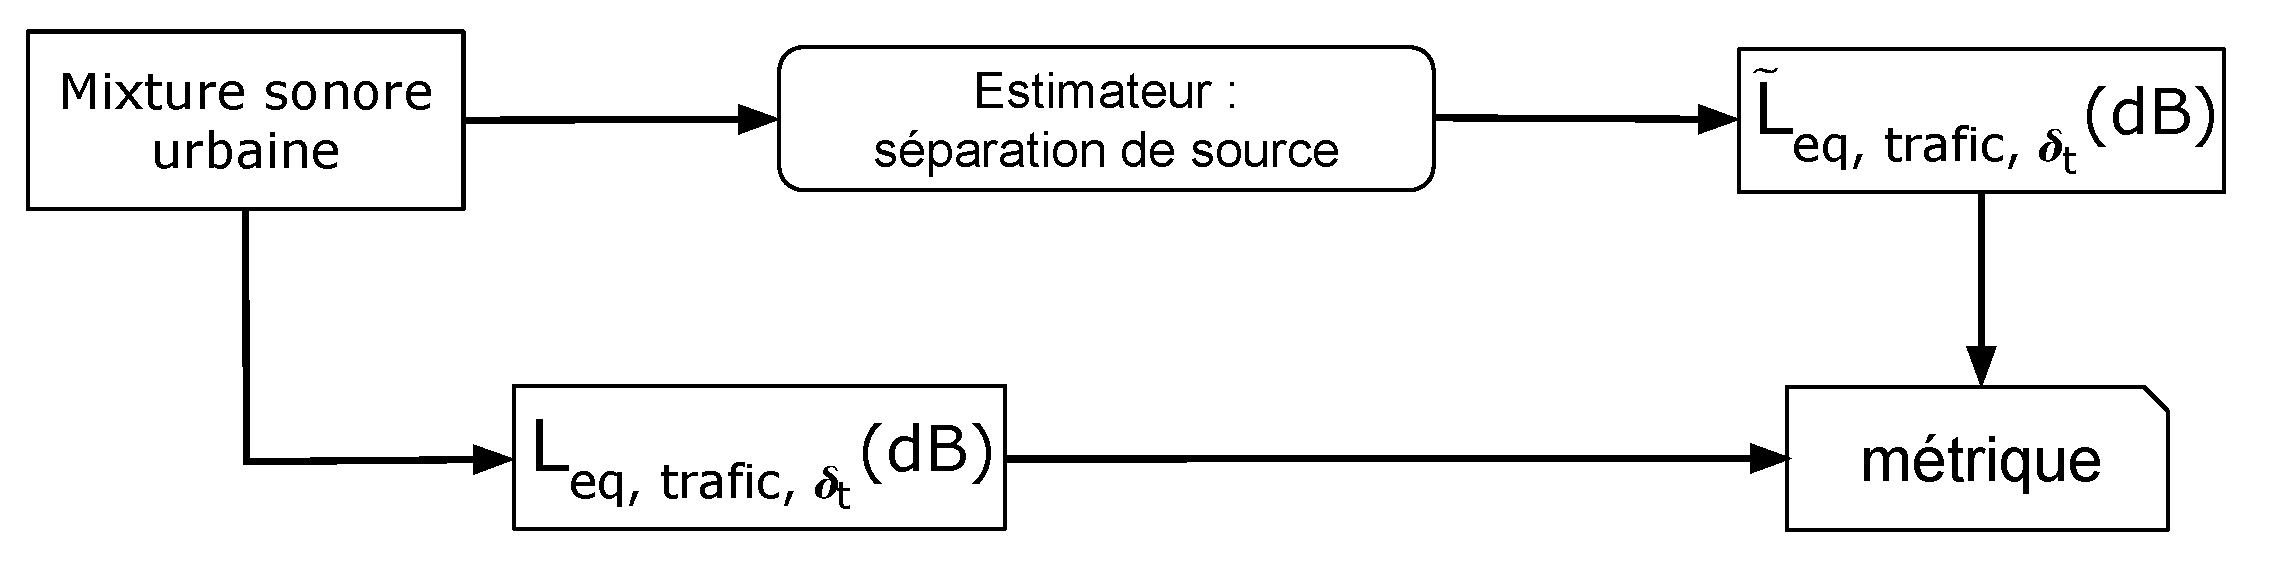
\includegraphics[width=.8\linewidth]{./figures/NMF/Bloc_diagram_estimateur_FR.pdf}
\caption{Schéma-bloc de l'estimation du niveau sonore du bruit de trafic.}
\label{fig:rappel_estimateur}
\end{figure}

Le corpus de scènes sonores, présenté dans \ref{part:corpus_ambiance}, est composé, pour rappel, de 6 sous-corpus : \textit{alerte}, \textit{animaux}, \textit{climat}, \textit{humain}, \textit{transport}, \textit{mécanique} (abrégés respectivement \textit{al.}, \textit{an.}, \textit{cl.}, \textit{hu.}, \textit{tr.} \textit{me.}). Chaque sous-corpus est lui-même divisé en 5 sous-ensembles qui comprennent, chacun, 25 mixtures sonores $M_i$ de 30 secondes, comprenant une classe de son \textit{trafic} (qui inclut le bruit de fond routier ainsi que les évènements sonores \textit{passages de voitures}), $S_{tr.}$, et une classe de son \textit{interférante} (qui regroupe tous les autres sources sonores), $S_{int.}$ :

\begin{equation}
M_i = S_{tr.,i}+S_{int.,i}.
\end{equation}

Dans chacun des 5 sous-ensembles sous-ensemble, le niveau sonore du signal \textit{trafic}, $L_{eq,tr.}$ est calibré par rapport au niveau sonore de la classe de son \textit{interférante}, $L_{eq,int.}$ tel que :

\begin{equation}
TIR = L_{eq,tr.} - L_{eq,int.}
\end{equation}

avec 5 valeurs $TIR \in \lbrace -12,~-6,~0,~6,~12 \rbrace$ dB. Ce corpus permet de tester les performances de la NMF et son comportement face à différentes sources sonores avec une prédominance variable du trafic routier. En tout, le corpus est composé de 750 scènes (6 sous-corpus $\times$ 5 $TIR$ $\times$ 25 scènes) pour une durée totale de 6h30.

Pour chaque $TIR$ et chaque sous-corpus, les 25 scènes $i$ sont soumises à un estimateur qui détermine le niveau sonore \textit{trafic} de l'intégralité de la scène en dB,  $\tilde{L}_{eq,tr., i}$. Les 25 niveaux sonores sont ensuite comparés aux niveaux sonores exacts respectifs, $L_{eq,tr., i}$ au travers de la métrique $MAE$ (équation \ref{eq:mae}), définie dans la partie \ref{sect:methode}. Il est ensuite possible de déterminer les performances d'un estimateur sur l'ensemble des 6 sous-corpus pour chaque $TIR$ en calculant sa moyenne :

\begin{equation}\label{eq:mae_tir}
MAE_{TIR} = \frac{\sum_{i = 1}^6 MAE_{i}}{6}.
\end{equation}

Il est enfin possible de calculer une erreur globale sur l'intégralité du corpus \textit{Ambiance}  :

\begin{equation}\label{eq:mae_g}
MAE_{g} = \frac{\sum_{i = 1}^6 \sum_{j = 1}^5 MAE_{i,j}}{6 \times 5}.
\end{equation}

L'erreur $MAE_g$ traduit l'erreur moyenne de l'estimateur faite sur l'intégralité du corpus d'évaluation et donc celle qui serait faite si aucune connaissance \textit{a priori} sur l'environnement sonore n'était disponible.

\section{Estimateur baseline}
Dans un premier temps, un estimateur de référence (ou \textit{baseline} en anglais) est nécessaire afin de comparer les performances de la NMF. La baseline choisie est un filtre passe-bas de fréquence de coupure $f_c$. L'hypothèse faite est que l'énergie située dans la bande passante est assimilable au signal \textit{trafic}, $\tilde{L}_{eq,trafic}$. Le choix de cet outil est justifié par la présence de composantes basses-fréquences (principalement en dessous de 1000 Hz) dans les signaux trafic. Supprimer l'énergie au-delà parait donc une première approche envisageable. %De plus, c'est une méthode qui pourrait être choisie par défaut.
Cet estimateur consiste à représenter une mixture $M_i$ sous la forme d'un spectrogramme puis à rejeter toutes les trames fréquentielles supérieures à $f_c$. La Figure \ref{fig:baseline} résume les étapes intervenant pour cet estimateur.

\begin{figure}[hbtp]
\centering
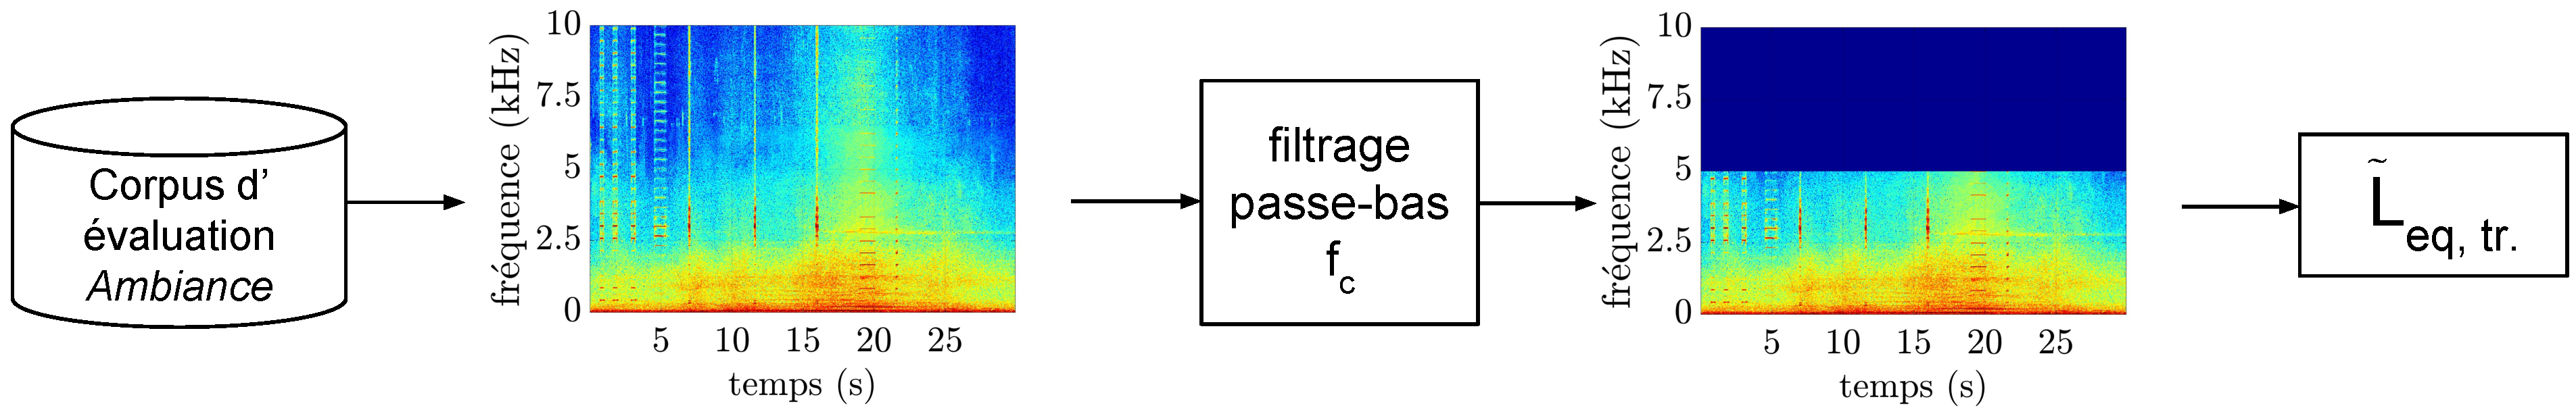
\includegraphics[width=\linewidth]{./figures/NMF/filtre_principe.pdf}
\caption{Principe de l'estimateur \textit{baseline}  pour une mixture sonore filtrée à $f_c$ = 5kHz.}
\label{fig:baseline}
\end{figure}

Les fréquences de coupure choisies sont $f_c \in \lbrace 100, 500, 1k, 2k, 5k, 10k, 20k \rbrace$ Hz. Le cas où $f_c = 20$ kHz correspond finalement au cas où aucun traitement du signal n'est réalisé sur les fichiers audio et où toutes les sources présentes sont assimilées au trafic, ce qui correspond à l'utilisation actuellement faite des mesures pour la correction de cartes de bruits issues de modèles prédictifs.

%\ml{je viens de lire sur la mesure d'impact des éoliennes, et ils utilisent des termes comme niveau ambient, résiduel ou d'émergence, ce serait peut etre approprié des les utiliser.}

\section{Estimateur basé sur la NMF}
Le second estimateur est celui basé sur la NMF, présentée dans le chapitre \ref{chap:NMF}. Pour rappel, cette méthode consiste à approximer le spectrogramme $\mathbf{V}$ d'un signal audio par le produit de deux matrices, $\mathbf{W}$, un dictionnaire de spectres sonores, et $\mathbf{H}$, une matrice d'activation temporelle. La Figure \ref{fig:nmf_ambiance} rappelle les différentes étapes présentes dans cet estimateur.

\begin{figure}[ht]
\centering
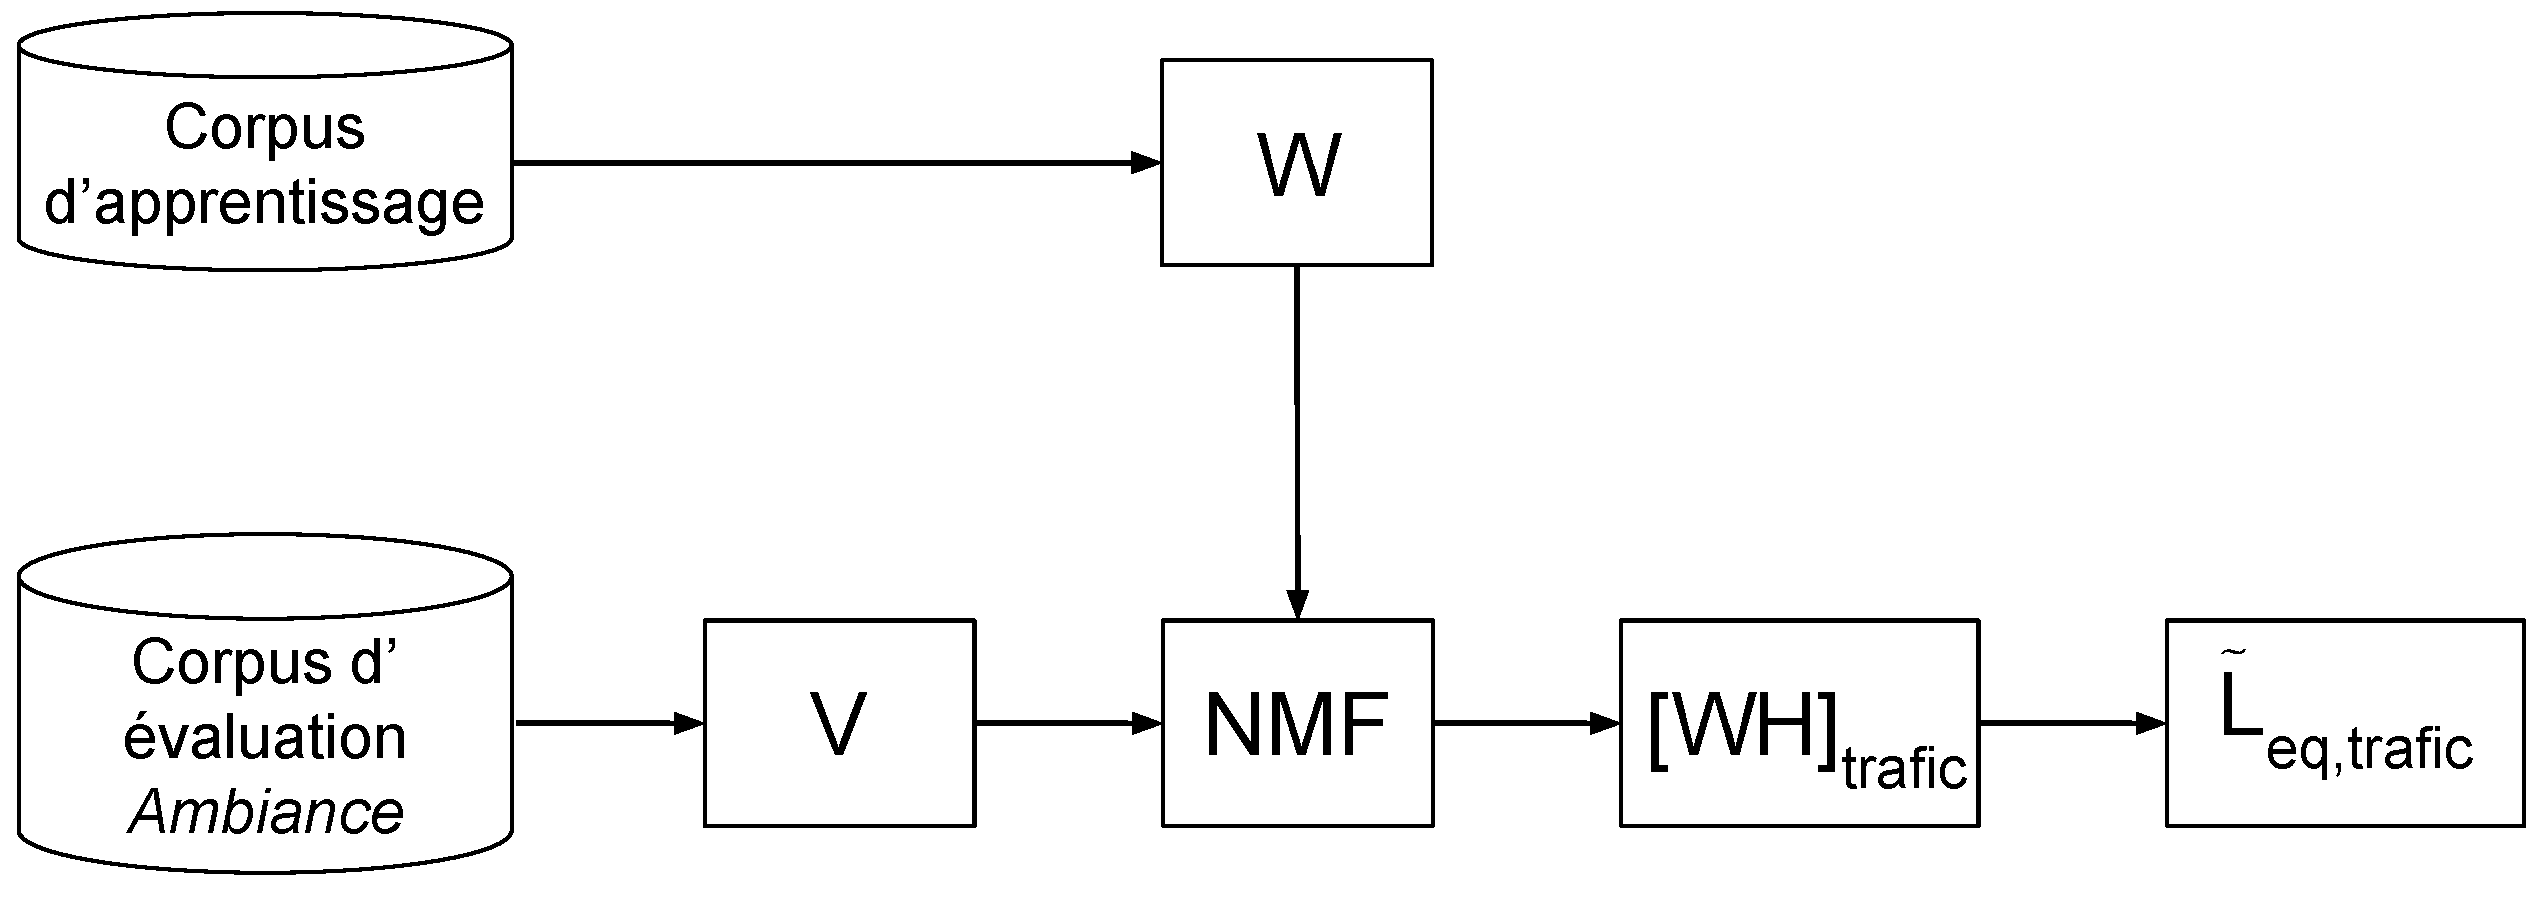
\includegraphics[width=0.7\linewidth]{./figures/NMF/NMF_ambiance.pdf}
\caption{Diagramme en blocs de l'estimateur NMF sur le corpus d'évaluation \textit{Ambiance}.}
\label{fig:nmf_ambiance}
\end{figure}


\subsection{Constitution du dictionnaire} 

Dans un premier temps, le dictionnaire $\mathbf{W}$ est construit, à partir d'un corpus d'apprentissage composé de 53  enregistrements audio des passages des voitures Renault Scénic et Dacia Sandero. Ces enregistrements ont été réalisés sur la piste d'essais de l'Ifsttar dans les mêmes conditions d'enregistrements que les 2 véhicules composants le corpus élémentaire de \textit{SimScene} (voir partie \ref{part:voiture_record}). Ces 53 échantillons audio issus des enregistrements ne sont pas ceux utilisés dans la création des scènes sonores afin d'éviter tout problème de sur-apprentissage.

\begin{figure}[hbtp]
\centering
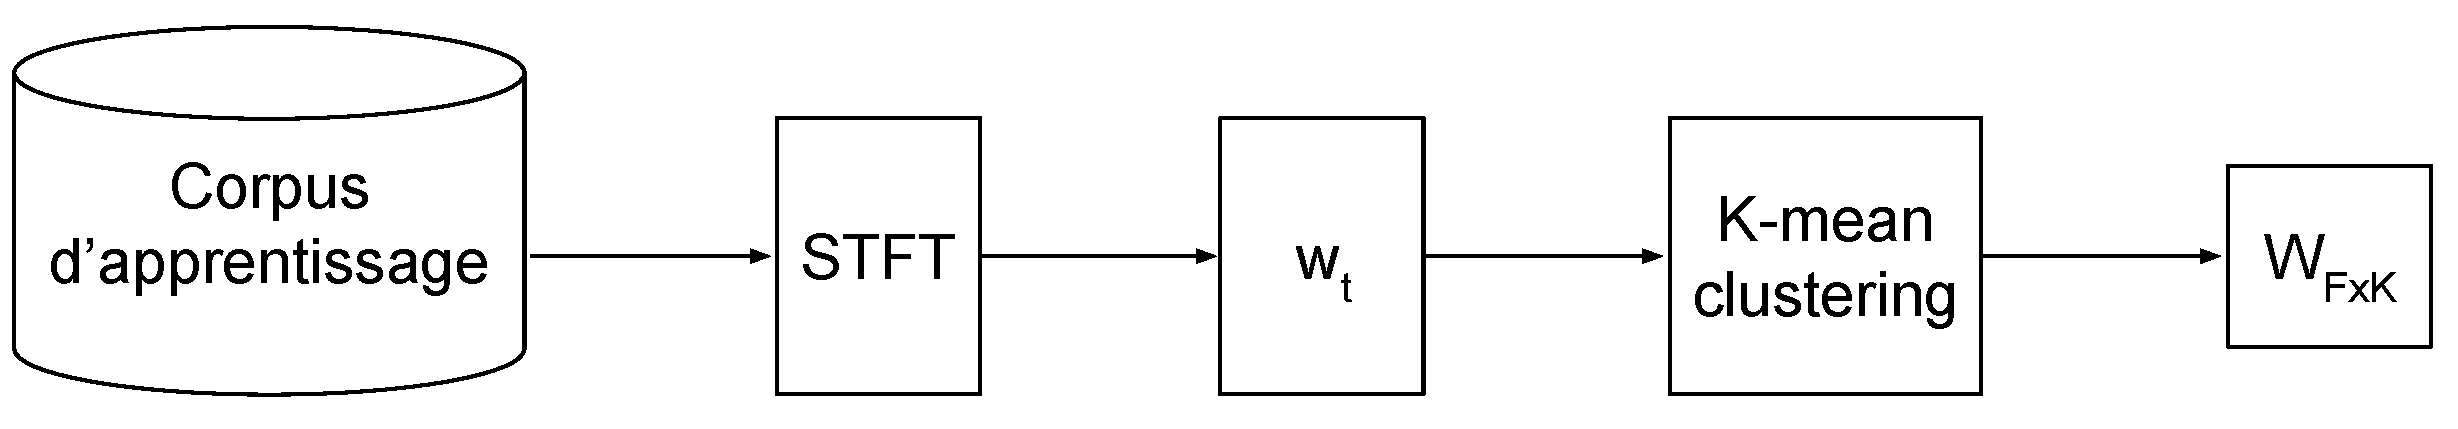
\includegraphics[width=.9\linewidth]{./figures/NMF/creation_dictionaire.pdf}
\caption{Diagramme en blocs de la création du dictionnaire.}
\label{fig:creation_W}
\end{figure}

La constitution du dictionnaire est réalisée en trois étapes, résumées dans le diagramme en blocs montré Figure \ref{fig:creation_W} :
\begin{itemize}
\item chaque fichier audio est représenté au travers d'un spectrogramme, obtenu par une Transformée de Fourier à Court Terme (nombre de point $w = 2^{12}$ avec 50 $\%$ de recouvrement). Cette première étape permet d'obtenir pour chaque échantillon audio, de durée différente, le même nombre de points en fréquences.
\item Chaque spectrogramme est ensuite découpé en plusieurs fenêtre temporelles de durée $w_t \in \lbrace 0.5,~ 1,~ 2\rbrace$ seconde(s). 
Dans chacune des fenêtres, la valeur efficace \textit{rms} sur chaque trame fréquentielle est calculée. Ce procédé, qui équivaut à un sous échantillonnage, a pour but d'obtenir différentes représentations des spectrogrammes initiaux avec une description du contenu spectral plus ou moins fine. Dans le cas où $w_t = 0,5$ s, les spectres sonores contiennent plus de détails que dans le cas où $w_t = 2$ s. Les étapes de ce processus sont résumées en Figure \ref{fig:decoupe_W} sur un extrait de 3 secondes.
\item Enfin, l'opération précédente générant un grand nombre d'éléments (2218 pour $w_t$ = 0,5 s, 505 pour $w_t$ = 2 s), une quantification vectorielle, opérée grâce à un algorithme de clustering $K$-means, est appliquée en vue de réduire ce nombre à $K = \lbrace 25,~50,~100,~200 \rbrace$ et d'éviter la présence d'informations redondantes. Les $K$ centroïdes obtenus par cet algorithme sont alors les éléments qui composent le dictionnaire $\mathbf{W}$.
\end{itemize}

En plus de ces étapes, on ajoute un cas où la valeur \textit{rms} est calculée sur l'ensemble des spectrogrammes ($w_t = all$). Des 53 fichiers audio du corpus d'apprentissage, 53 spectres sont générés. Cette opération permet de baser la construction du dictionnaire sur les enveloppes spectrales des fichiers audio \textit{trafic} et moins sur une description fine des spectres. Ces 53 spectres sont également soumis à l'algorithme de clustering mais avec cette fois, $K_{w_t = all} \in \lbrace 25,~ 50 \rbrace$.
L'ensemble de ces facteurs expérimentaux et leurs modalités sont résumés dans le Tableau \ref{tab:experimental_factorsNMF_ambiance}. L'intérêt de ces paramètres est de multiplier le nombre de format que peut prendre le dictionnaire pour ainsi estimer l'influence de la forme des composantes et leur nombre dans l'estimation du niveau sonore du trafic selon les différentes NMF. Enfin, chaque élément du dictionnaire $\mathbf{w}$, pour toutes les combinaisons testées, est normalisé selon la norme $\ell_1$ telle que 
$\Vert \mathbf{w} \Vert_1 = \sum_{f = 1}^{F} w_f =  1$.

\begin{figure}[hbtp]
\centering
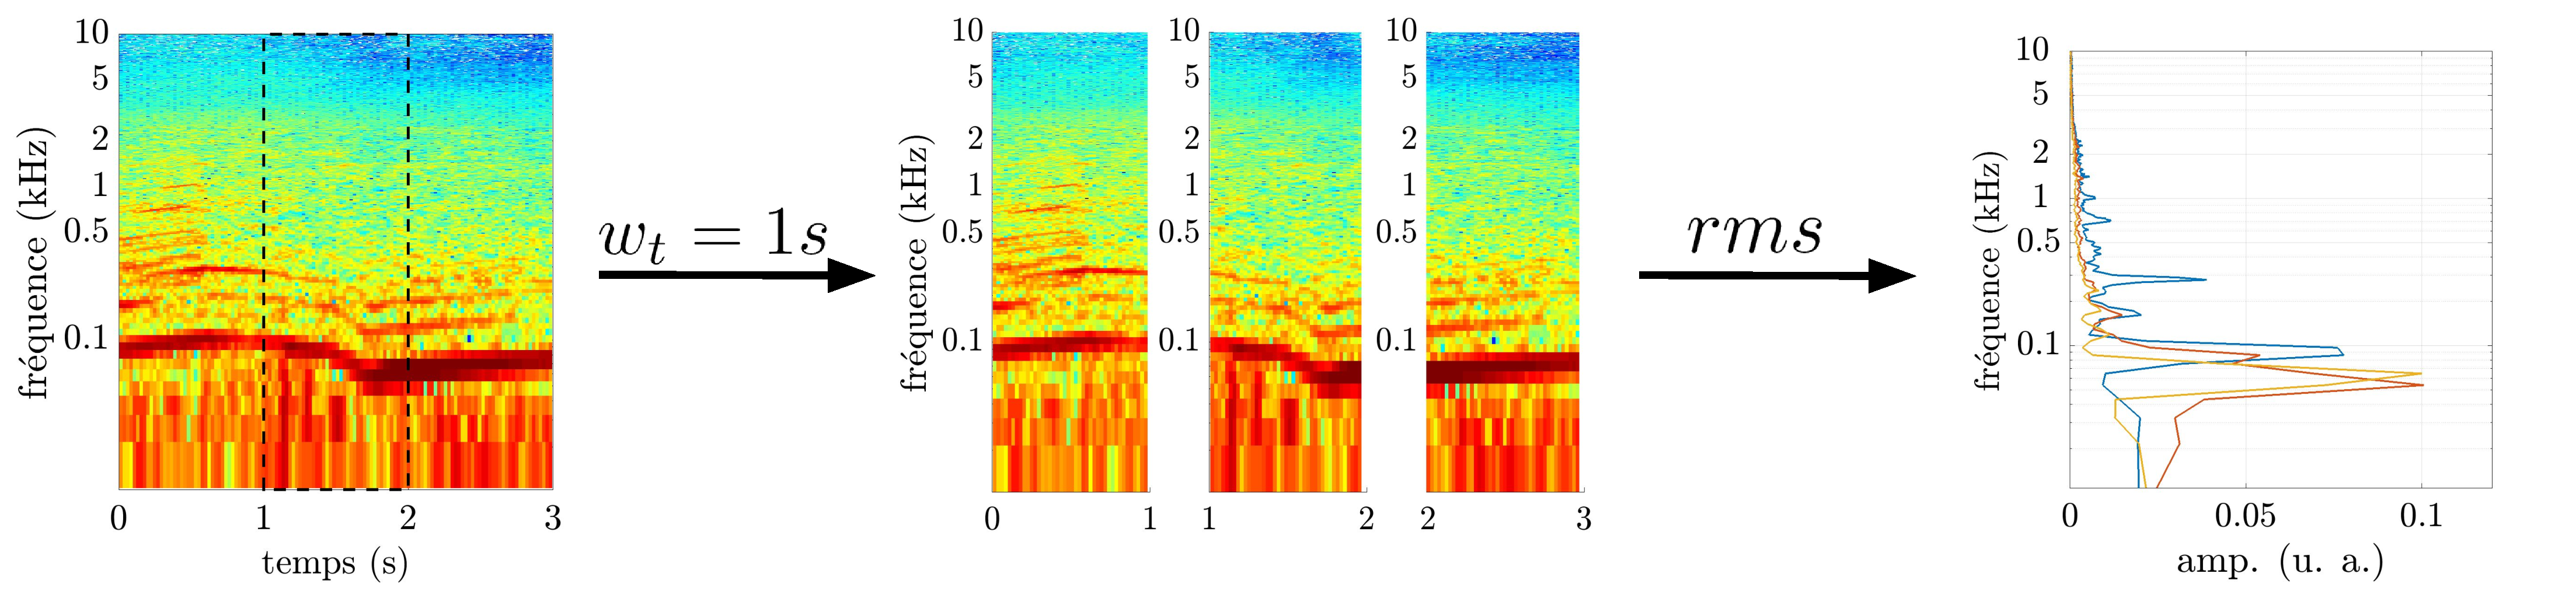
\includegraphics[width=\linewidth]{./figures/NMF/dictionaire_frame_FR.pdf}
\caption{Création des éléments de $\mathbf{W}$ sur un extrait de 3 secondes du passage d'une voiture pour une trame temporelle $w_t$ = 1 seconde. À gauche, le spectrogramme du signal audio avec, en pointillés, une fenêtre de découpe. Au centre, le signal découpé en trois trames et dont les valeurs \textit{rms} sont ensuite calculées générant 3 spectres.}
\label{fig:decoupe_W}
\end{figure}

\subsection{Réalisation de la NMF}

Chaque version du dictionnaire $\mathbf{W}$ est utilisé par l'estimateur du niveau de traffic. Cet estimateur est lui-même basé sur plusieurs versions de la NMF décrites précédemment (voir chapitre \ref{chap:NMF})  : la NMF supervisée (NMF SUP), semi-supervisée (NMF SEM) et initialisée-seuillée (NMF IS). Pour chaque NMF, 3 $\beta$-divergences sont utilisées : la distance Euclidienne ($\beta = 2$) (voir partie \ref{part:dist_EUC}, la divergence de Kullback-Leibler ($\beta = 1$) (partie \ref{part:div_KL}), et la divergence d'Itakura-Saïto ($\beta = 0$) (partie \ref{part:div_IS}). La NMF SUP dépend seulement des différentes versions du dictionnaire apprises et des valeurs de $\beta$. Le signal trafic est estimé selon l'équation \ref{eq:WH_trafic} à partir de la matrice $\mathbf{H}$ obtenue.
Dans le cas de la NMF SEM, le dictionnaire appris compose la partie fixe $\mathbf{W_s}$. Le nombre d'éléments du dictionnaire libre $\mathbf{W_r}$ est alors fixé à 2 ($J = 2$). Le signal \textit{trafic} est ensuite déterminé par le relation \ref{eq:WSHs_trafic}.
Enfin pour la NMF IS, les dictionnaires appris correspondent aux dictionnaires initiaux $\mathbf{W_0}$ qui seront ensuite mis à jour. À chaque itération, les éléments du dictionnaire sont également tous normalisés. Les dictionnaires obtenus $\mathbf{W'}$ sont ensuite soumis à l'étape d'extraction par seuillage qui implique également plusieurs facteurs expérimentaux :

\begin{itemize}
\item la représentation de la distance entre les dictionnaires initiaux et finaux $D_{\theta}(\mathbf{W_0} \Vert \mathbf{W'})$ (linéaire ou bien exprimé au travers d'une fonction sigmoïde ($\lambda = 2$)),
\item le type de seuillage appliqué (dur ou \textit{firm}),
\item les valeurs des différents seuils respectifs ($t_h$ pour le seuillage dur et $t_{f,1/2}$, les deux valeurs seuils pour le seuillage \textit{firm}). Des études préliminaires ont permis de réduire la plage des valeurs de ces seuils à $t_h \in \left[ 0,30~0,70 \right]$, $t_{f,1} \in \left[ 0,20~0,55 \right]$ et $t_{f,2} \in \left[ 0,35,~0,70 \right]$, chacun étant défini avec un pas de 0,01. Rappelons que pour le seuillage \textit{firm}, $t_{f,1} \leq t_{f,2}$.
\end{itemize}

Malgré la réduction du nombre d'éléments par l'algorithme $K$-means, la taille des matrices $\mathbf{W}$ et $\mathbf{V}$ reste importante en raison du nombre de trames fréquentielles ($F$ = 2049). En conséquence, ces deux matrices sont exprimées en bandes de tiers-d'octaves ce qui réduit les dimensions des matrices ($F_{1/3} = 29$). L'allure d'un spectre du passage d'une voiture en bandes fines et en tiers d'octaves est représenté en Figure \ref{fig:tiers_octaves}. La manipulation des matrices est alors plus rapide qu'avec les bandes fines et permet donc un gain en temps de calcul. Cette représentation a également d'autres intérêts :

\begin{itemize}
\item par son échelle logarithmique, elle décompose mieux les basses fréquences que les hautes fréquences ce qui permet de mieux focaliser la reconstruction du signal vers les bandes de fréquences d'intérêt.
\item Cette représentation est également couramment utilisée dans le domaine de l'acoustique urbaine et environnementale, à la différence des MFCC. Notamment tous les réseaux de mesures en ville déterminent des valeurs du niveaux sonores en bande de tiers d'octave. Cela en fait donc une représentation adaptée.
\end{itemize}

\begin{figure}[h]
\centering
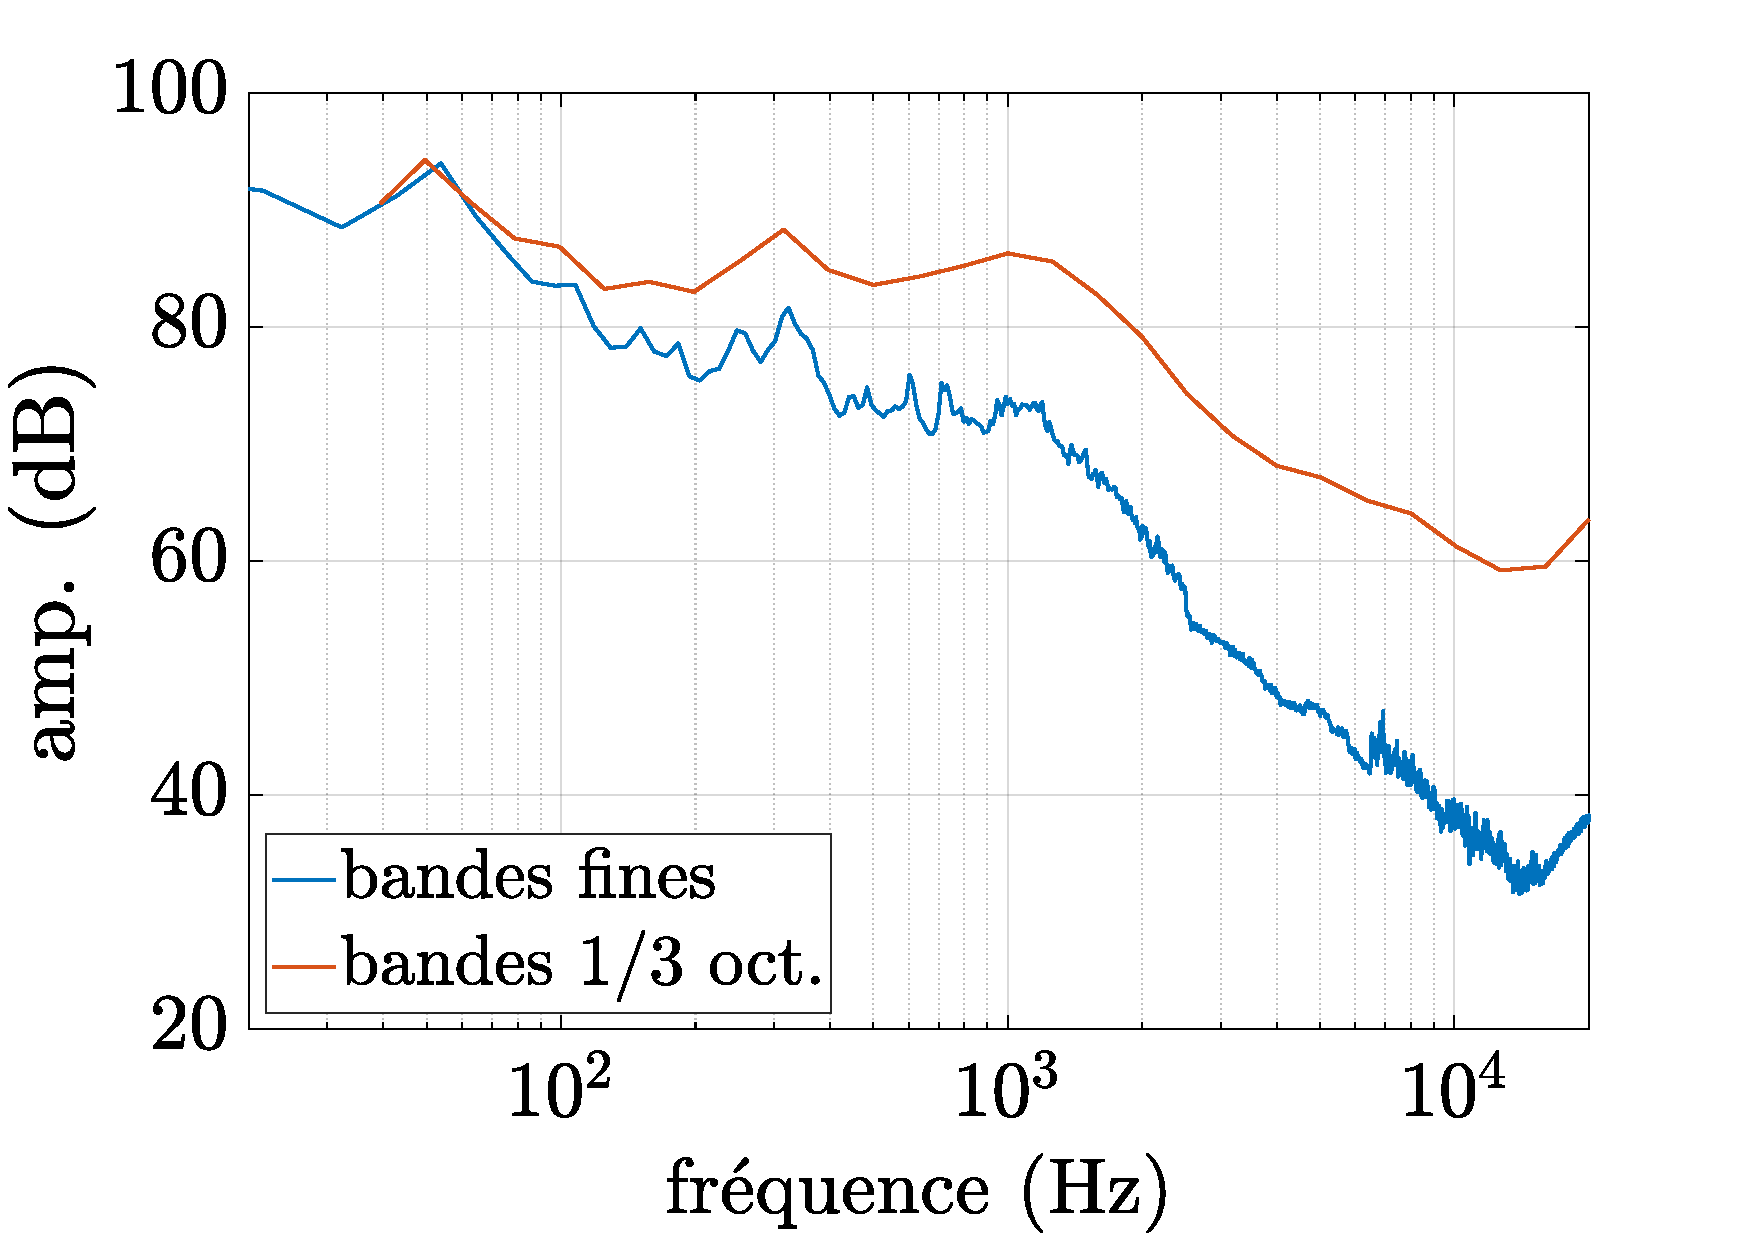
\includegraphics[width=0.5\linewidth]{./figures/NMF/bande_fine_tiers.pdf}
\caption{Spectre en fréquence du passage d'une voiture en bandes fines (2049 points) et en bandes de tiers d'octave (29 bandes).}
\label{fig:tiers_octaves}
\end{figure}

Enfin, le nombre d'itérations est fixé à 100 pour toutes les versions de la NMF étudiées.

\subsection{Résumé des facteurs expérimentaux}

De nombreux facteurs expérimentaux sont donc présents dans cette expérience, chacun ayant différentes modalités. Le Tableau \ref{tab:experimental_factorsNMF_ambiance} résume l'ensemble de ces paramètres dont les différents sous-corpus, valeurs du $TIR$ et facteurs expérimentaux liés aux estimateurs. La Figure \ref{fig:organigramme} représente les différents facteurs expérimentaux impliqués dans l'estimateur ainsi que leurs liens de dépendances.

\begin{figure}[h]
\centering
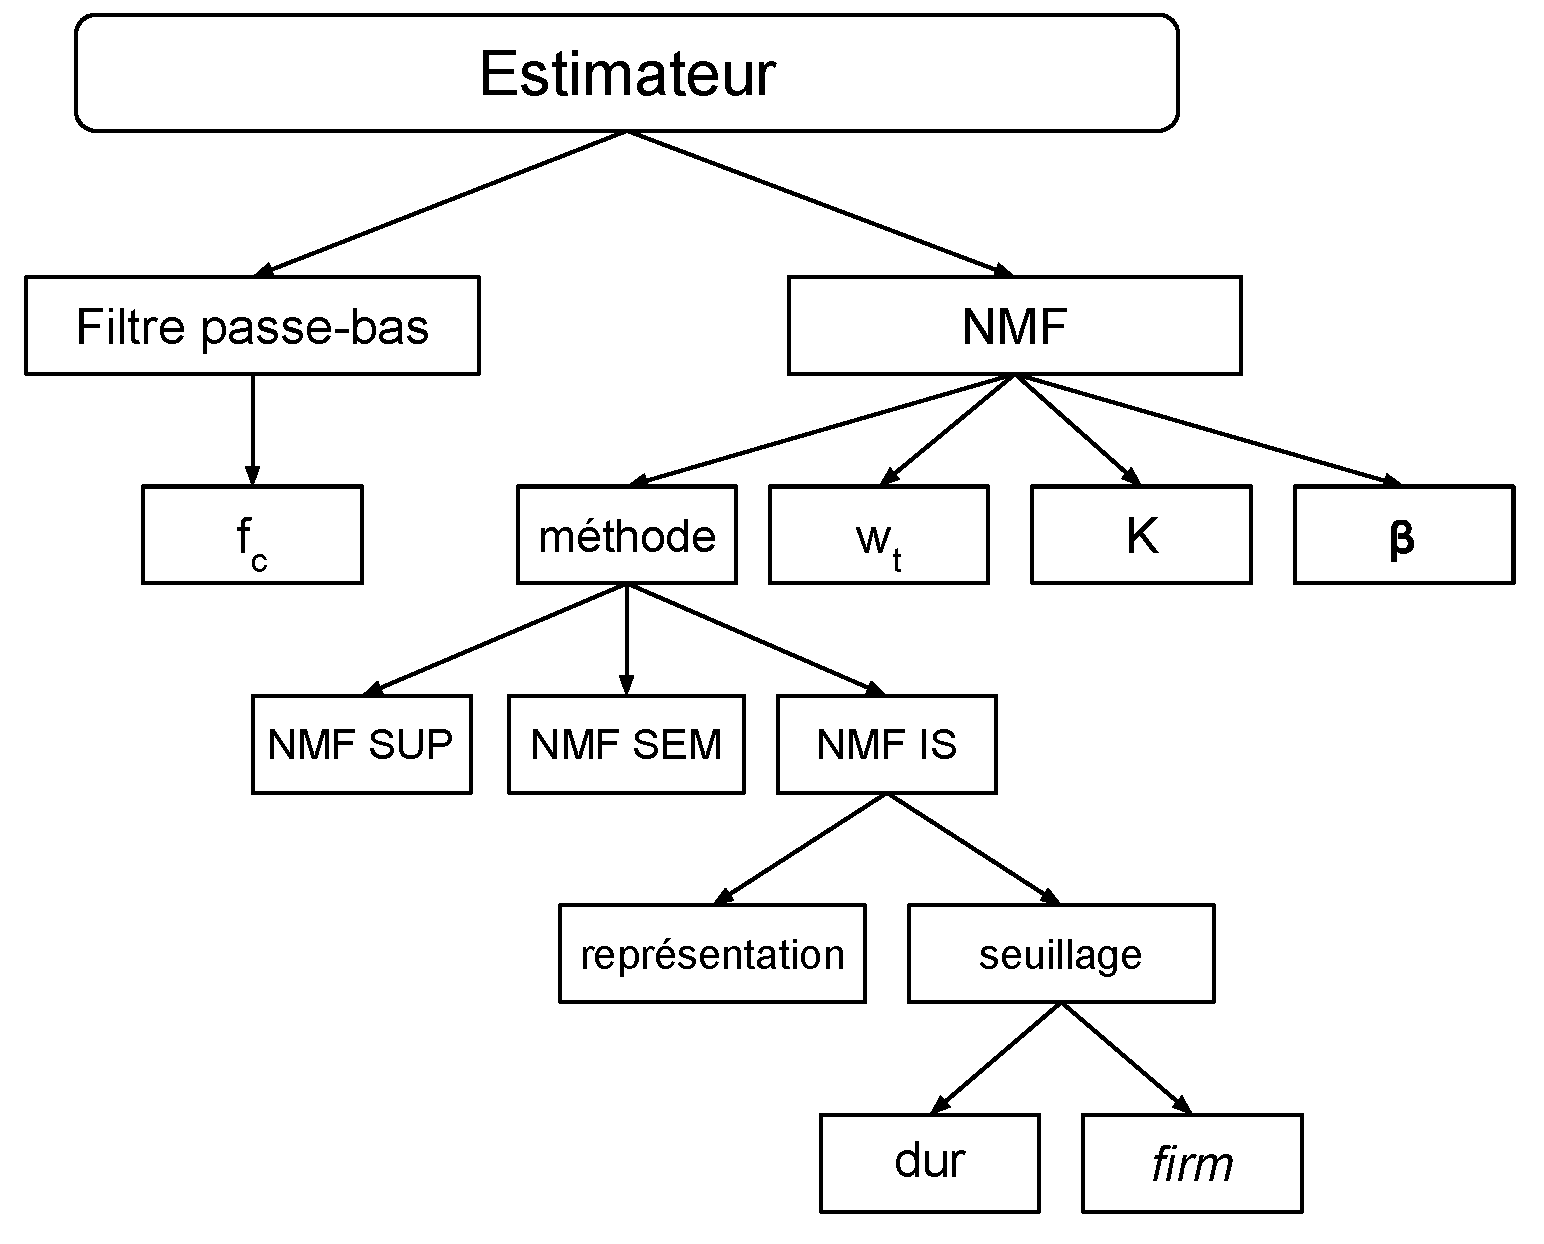
\includegraphics[width=0.8\linewidth]{./figures/NMF/facteurs_exp.pdf}
\caption{Organigramme des différents facteurs expérimentaux impliqués dans l'outil \textit{estimateur}.}
\label{fig:organigramme}
\end{figure}

\begin{table*}[h]
\centering
\caption{Facteurs expérimentaux et leurs modalités utilisés pour le corpus d'évaluation \textit{Ambiance}.}
\begin{tabularx}{17.5cm}{L{3cm}@{}C{12cm}@{}C{2cm}@{}}
	\hline
    \textbf{\begin{tabular}[c]{@{}l@{}}facteurs \\ expérimentaux \end{tabular}} & \textbf{modalités} & \begin{tabular}[c]{@{}C{2cm}@{}}\textbf{nombre de}\\ \textbf{modalités}\end{tabular}\\ \toprule
\end{tabularx}

\begin{tabularx}{17.5cm}{L{2.8cm}@{}@{}C{2cm}@{}@{}C{2cm}@{}@{}C{2cm}@{}@{}C{2cm}@{}@{}C{2cm}@{}@{}C{2.2cm}@{}C{2cm}}
   \textbf{sous-corpus} & alerte (al.) & animaux (an). & climat (cl.) &  humain (hu.) & transport (tr.) & mécanique (me.) & 6\\
\end{tabularx}

\begin{tabularx}{17.5cm}{L{2.8cm}@{}@{}C{2.435cm}@{}@{}C{2.435cm}@{}@{}C{2.435cm}@{}@{}C{2.435cm}@{}@{}C{2.435cm}@{}C{2cm}}
\rowcolor[HTML]{C0C0C0}
   $TIR$ (dB) & -12 & -6 & 0 & 6 & 12 & 5\\
\end{tabularx}

\begin{tabularx}{17.5cm}{L{3cm}@{}C{3cm}@{}@{}C{3cm}@{}@{}C{3cm}@{}@{}C{3cm}@{}C{2cm}@{}}
  \textbf{estimateur} & filtre passe bas & NMF SUP & NMF SEM & NMF IS & 4\\
\end{tabularx}

\begin{tabularx}{17.5cm}{L{3cm}@{}@{}C{1.71cm}@{}@{}C{1.71cm}@{}@{}C{1.71cm}@{}@{}C{1.71cm}@{}@{}C{1.71cm}@{}@{}C{1.71cm}@{}@{}C{1.71cm}@{}C{2cm}@{}}
\rowcolor[HTML]{C0C0C0}
   $f_c$ (kHz) & 0,1 & 0,5 & 1 & 2 &  5 & 10 & 20 & 7\\
\end{tabularx}

\begin{tabularx}{17.5cm}{L{3cm}@{}C{3cm}@{}@{}C{3cm}@{}@{}C{3cm}@{}@{}C{3cm}@{}C{2cm}@{}}
    $w_t$ (s)& 0,5 & 1 & 2 & \textit{all} & 4\\
\end{tabularx}

\begin{tabularx}{17.5cm}{L{3cm}@{}C{3cm}@{}@{}C{3cm}@{}@{}C{3cm}@{}@{}C{3cm}@{}C{2cm}@{}}
	\rowcolor[HTML]{C0C0C0}
    $K$ & 25 & 50 & 100 & 200 & 4\\
\end{tabularx}

\begin{tabularx}{17.5cm}{L{3cm}@{}C{4cm}@{}@{}C{4cm}@{}@{}C{4cm}@{}C{2cm}@{}}
   $\beta$ & 0 & 1 & 2 & 3\\
\end{tabularx}

\begin{tabularx}{17.5cm}{L{3cm}@{}C{6cm}@{}@{}C{6cm}@{}C{2cm}@{}}
	\rowcolor[HTML]{C0C0C0}
   \textbf{représentation} & linéaire & sigmoïde & 2\\
\end{tabularx}

\begin{tabularx}{17.5cm}{L{3cm}@{}C{6cm}@{}@{}C{6cm}@{}C{2cm}@{}}
   \textbf{seuillage} & dur & \textit{firm} & 2\\
\end{tabularx}

\begin{tabularx}{17.5cm}{L{3cm}@{}C{12cm}@{}C{2cm}@{}}
	\rowcolor[HTML]{C0C0C0}
	\textbf{seuil dur} $\mathbf{t_h}$ & de 0,30 à 0,60 avec un pas de 0.01 & 31\\
\end{tabularx}

\begin{tabularx}{17.5cm}{L{3cm}@{}C{12cm}@{}C{2cm}@{}}
   \textbf{seuil firm} $\mathbf{t_{f,1}}$ & de 0,20 à 0,55 avec un pas de 0,01 & 36\\
\end{tabularx}

\begin{tabularx}{17.5cm}{L{3cm}@{}C{12cm}@{}C{2cm}@{}}
	\rowcolor[HTML]{C0C0C0}
   \textbf{seuil firm} $\mathbf{t_{f,2}}$ & de 0,35 à 0,70 avec un pas de 0,01 & 36\\
   \bottomrule
\end{tabularx}
\label{tab:experimental_factorsNMF_ambiance}
\end{table*}

Pour l'estimateur filtre, c'est donc 210 combinaisons qui sont réalisées (6 sous-corpus $\times$ 5 $TIR$ $\times$ 7 $f_c$). Dans le cas de la NMF SUP et SEM, ce sont respectivement 1260 combinaisons qui sont évaluées (6 sous-corpus $\times$ 5 $TIR$ $\times$ (3 $w_t$ $\times$ 4 $K$ + 1 $w_t$ $\times$ 2 $K$ ) $\times$ 3 $\beta$). Dans le cas de la NMF IS, ce nombre est beaucoup plus élevé (2 789 640) en raison des nombreuses valeurs seuils (6 sous-corpus $\times$ 5 $TIR$ $\times$ (3 $w_t$ $\times$ 4 $K$ + 1 $w_t$ $\times$ 2 $K$ ) $\times$ 3 $\beta$ $\times$ 2 représentation $\times$ (31 + 1076)).

Les calculs exhaustifs de toutes les combinaisons expérimentales sont réalisés avec le logiciel Matlab à l'aide de l'outil expLanes\footnote{\url{http://mathieulagrange.github.io/expLanes}} qui permet la réalisation d'expériences numériques, de gérer la distribution des nombreux facteurs expérimentaux et leur modalités et de collecter les nombreux résultats générés. %L'ordinateur menant les calculs est équipé d'un processeur Intel Core i7 (CPU 2,40 GHz).

\section{Performances de l'estimateur \textit{baseline}}

Les résultats issus de l'estimateur \textit{baseline} sont d'abord présentés. Dans un premier temps, les erreurs $MAE_g$ (équation \ref{eq:mae_g}) générées par les estimations réalisées par chaque fréquence de coupure sont résumées dans le Tableau \ref{tab:resuls_ambiance_filtre} ainsi que les erreurs $MAE_{TIR}$.

\begin{table}[h]
\centering
\caption{Erreurs $MAE_g$ de l'estimateur \textit{baseline} selon $f_c$ sur l'ensemble du corpus \textit{Ambiance} et pour chaque $TIR$. En gras-rouge l'erreur $MAE_g$ la plus faible, en gras-noir, les erreurs $MAE_{TIR}$ les plus faibles selon les fréquences $f_c$.}
\label{tab:resuls_ambiance_filtre}
\resizebox{\textwidth}{!}{%
\begin{tabular}{lcccccc}
\toprule
$f_c$ (Hz) & $MAE_g$ & $MAE_{-12}$ & $MAE_{-6}$ & $MAE_{0}$ & $MAE_{6}$ & $MAE_{12}$ \\
\midrule
 100 & 3,21 ($\pm$ 1,06) & \textbf{4,55 ($\pm$ 1,55)} & \textbf{2,92 ($\pm$ 0,42)} & 2,36 ($\pm$ 0,71) & 2,97 ($\pm$ 0,41) & 3,25 ($\pm$ 0,32)\\
 \rowcolor[HTML]{C0C0C0}
 500 & \textbf{\textcolor{red}{2,89 ($\pm$ 2,84)}} & 7,39 ($\pm$ 3,00) & 3,44 ($\pm$ 1,65) & \textbf{1,17 ($\pm$ 0,24)} & 1,03 ($\pm$ 0,26) & 1,45 ($\pm$ 0,13) \\
 1000 & 3,36 ($\pm$ 3,63) & 9,44 ($\pm$ 2,03) & 4,78 ($\pm$ 1,34) & 1,62 ($\pm$ 0,54) & \textbf{0,36 ($\pm$ 0,10)} & 0,61 ($\pm$ 0,06) \\
 \rowcolor[HTML]{C0C0C0}
 2000 & 3,83 ($\pm$ 4,01) & 10,30 ($\pm$ 1,57) & 5,65 ($\pm$ 1,05) & 2,25 ($\pm$ 0,49) & 0,62 ($\pm$ 0,15) & \textbf{0,11 ($\pm$ 0,02)}\\
 5000 & 4,51 ($\pm$ 4,43) & 11,95 ($\pm$ 0,20) & 6,70 ($\pm$ 0,16) & 2,82 ($\pm$ 0,10)  & 0,87 ($\pm$ 0,04) & 0,20 ($\pm$ 0,02)\\
 \rowcolor[HTML]{C0C0C0}
10000 & 4,64 ($\pm$ 4,51) & 12,19 ($\pm$ 0,08) & 6,90 ($\pm$ 0,07) & 2,95 ($\pm$ 0,05) & 0,92 ($\pm$ 0,02) & 0,22 ($\pm$ 0,01)\\
20000 & 4,69 ($\pm$ 4,52) & 12,25 ($\pm$ 0,05) & 6,96 ($\pm$ 0,05) & 3,00 ($\pm$ 0,03) & 0,97 ($\pm$ 0,01) & 0,26 ($\pm$ 0,00)\\
\bottomrule
\end{tabular}}
\end{table}

La plus faible erreur $MAE_g$ sur l'intégralité du corpus est obtenue pour une fréquence de coupure $f_c$ = 500 Hz ($MAE_g$ = 2,89 ($\pm$ 2,84)).
\`A l'inverse, c'est naturellement pour la fréquence de coupure de 20 kHz que l'erreur est la plus importante puisque l'intégralité des sources sonores est considérée ($MAE_g$ = 4,69 ($\pm$ 4,52)).
En détaillant les erreurs $MAE_{TIR}$, on constate que la fréquence de coupure correspondant à l'erreur minimale évolue en fonction de la prédominance du trafic : la fréquence de coupure $f_c$ augmente avec le $TIR$.
Avec l'augmentation de la présence des voitures, il est nécessaire d'augmenter la fréquence $f_c$ afin de conserver le plus possible l'énergie sonore de cette source. \`A l'opposé, lorsque le $TIR$ est négatif, le filtre le plus performant sera celui qui est susceptible d'éliminer suffisamment d'énergie pour ne pas prendre en considération les sources sonores interférantes. Ce comportement est caractéristique d'un outil de détection qui peut soit réaliser des faux positifs (ce qui correspond à la prise en compte de la classe interférante dans le signal \textit{trafic}) soit rater des évènements (ce qui revient ici à supprimer trop d'énergie du signal \textit{trafic}).
Dans le cas du filtre $f_c$ = 500 Hz,  on détaille les erreurs par sous-corpus et $TIR$ (Figure \ref{fig:filtre_amb_tir}).

\begin{figure}[h!]
\centering
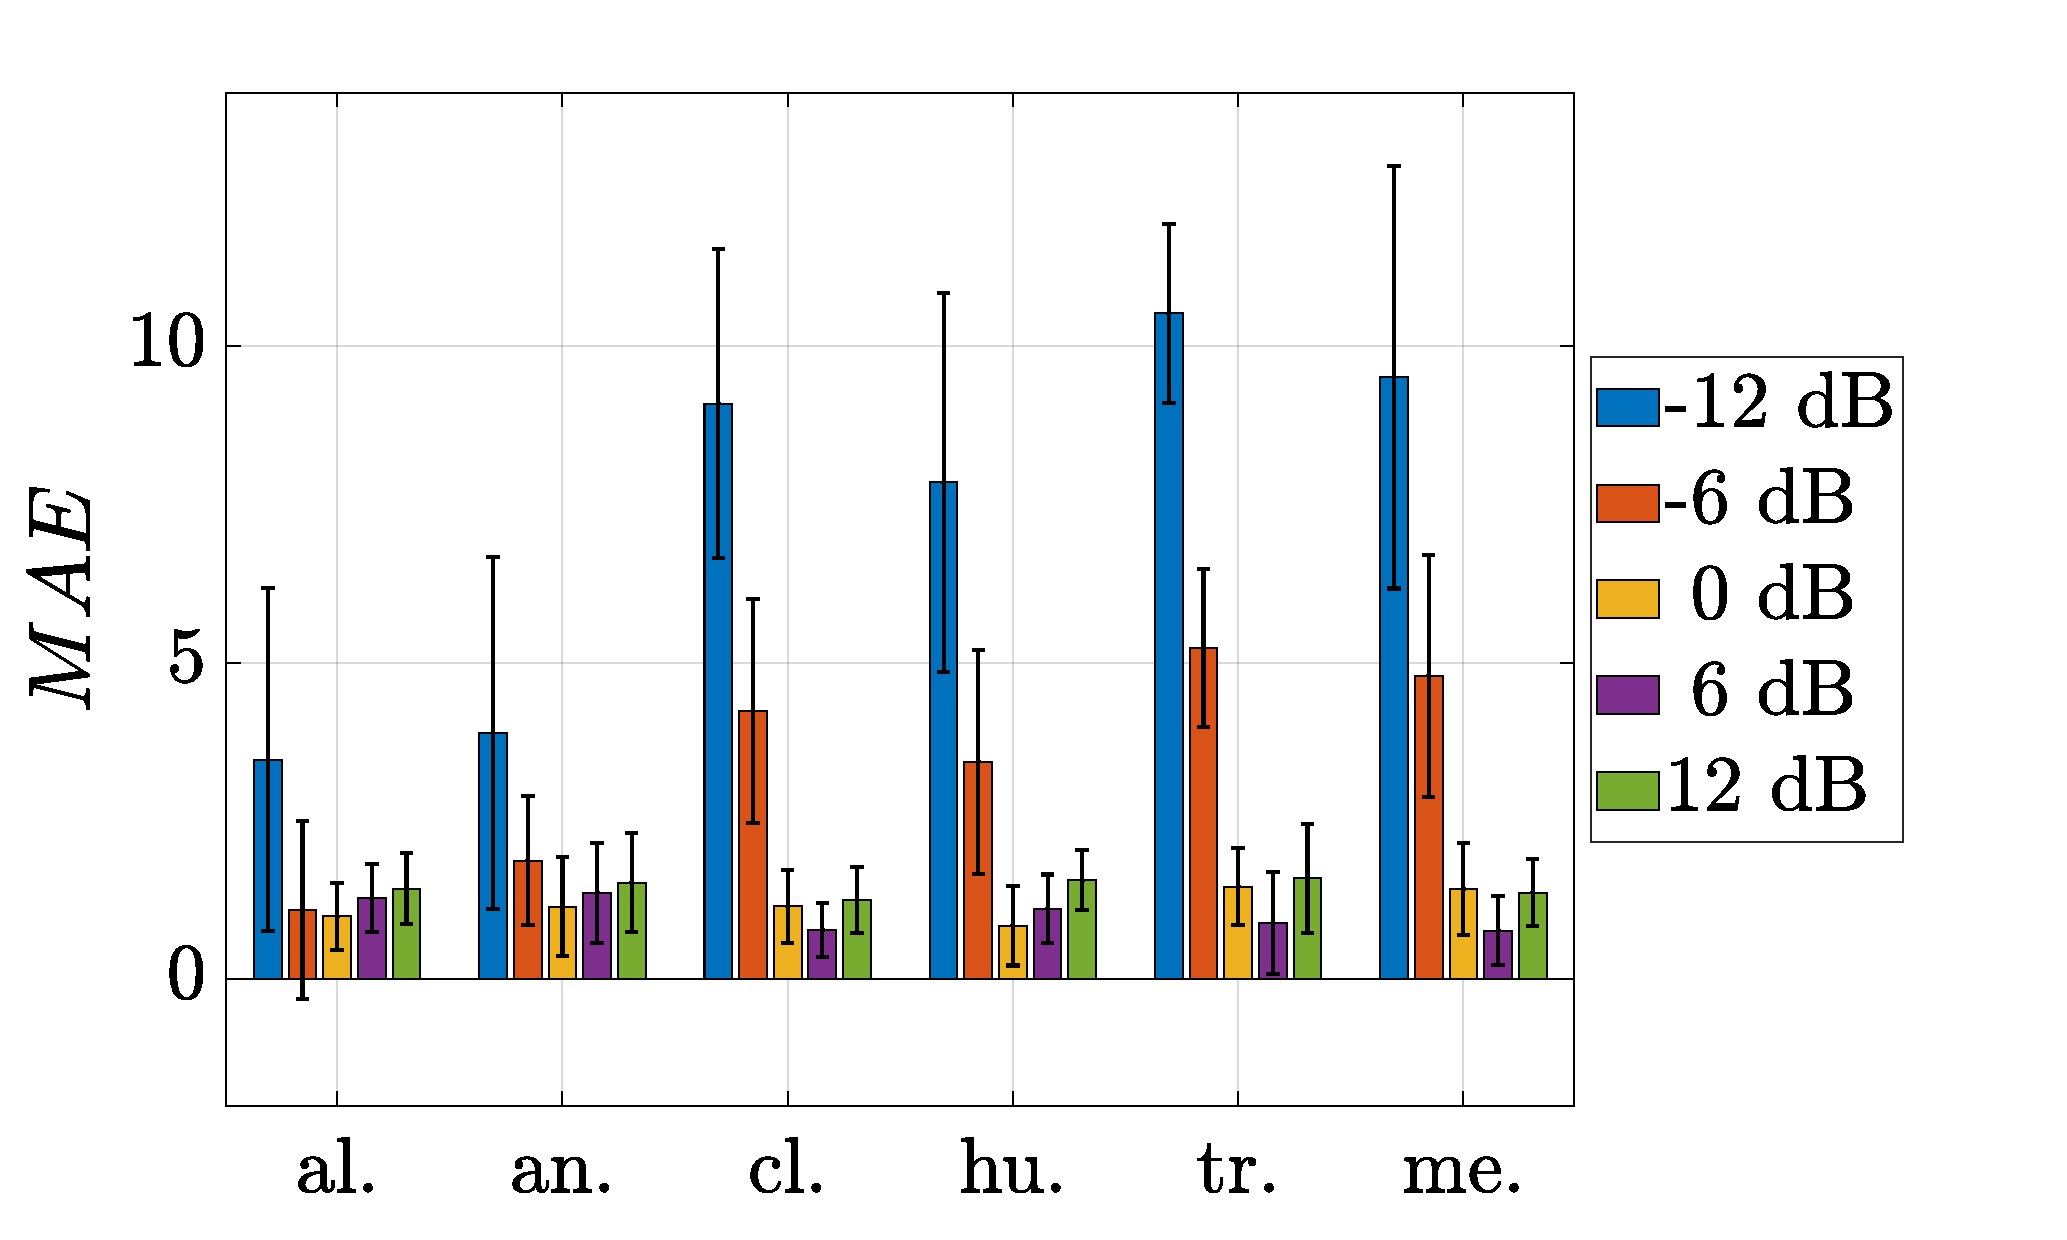
\includegraphics[width=0.7\linewidth]{./figures/resultats/amb_filtre_500_bar.pdf}
\caption{Erreurs $MAE$ pour chaque sous-corpus et chaque $TIR$ pour l'estimateur filtre passe-bas à la fréquence de coupure $f_c$ = 500 Hz.}
\label{fig:filtre_amb_tir}
\end{figure}

Les plus fortes erreurs sont obtenues pour les valeurs du $TIR$ négatives (-12 dB et -6 dB) notamment pour les sous-corpus \textit{climat}, \textit{humain}, \textit{transport} et \textit{mécanique} qui contiennent des composantes situées dans les basses fréquences. L'erreur du filtre à 500 Hz est alors due à la présence d'une partie de l'énergie de la classe interférante dans la bande passante. Dans ces $TIR$, le filtre se révèle plus efficace pour les sous-corpus \textit{alerte} et \textit{animaux}, puisque les spectres sonores des classes de sons interférantes sont plus aigus et donc mieux filtrés.
Avec l'augmentation du $TIR$, lorsque le trafic devient prédominant, l'erreur diminue pour chaque sous-corpus ($MAE <$ 2 dB) avec systématiquement une erreur $MAE$ plus élevée à $TIR$ = 12 dB qu'à $TIR$ = 6 dB. Cette erreur est ici dûe à la suppression d'une trop grande quantité d'énergie de la composante \textit{trafic}. Dans le cas extrême de $f_c$ = 20 kHz (Figure \ref{fig:filtre_amb_tir_20k}), cette erreur disparait logiquement : la source trafic étant principale, en conservant toute l'énergie sonore, l'estimation du trafic en devient meilleure. Mais dans les cas où le $TIR$ est négatif, l'erreur augmente significativement. On note que, pour ce filtre, l'erreur revient finalement à la somme des niveaux sonores des 2 classes de sons (équation \ref{eq:erreur20k}).

\begin{figure}[h!]
\centering
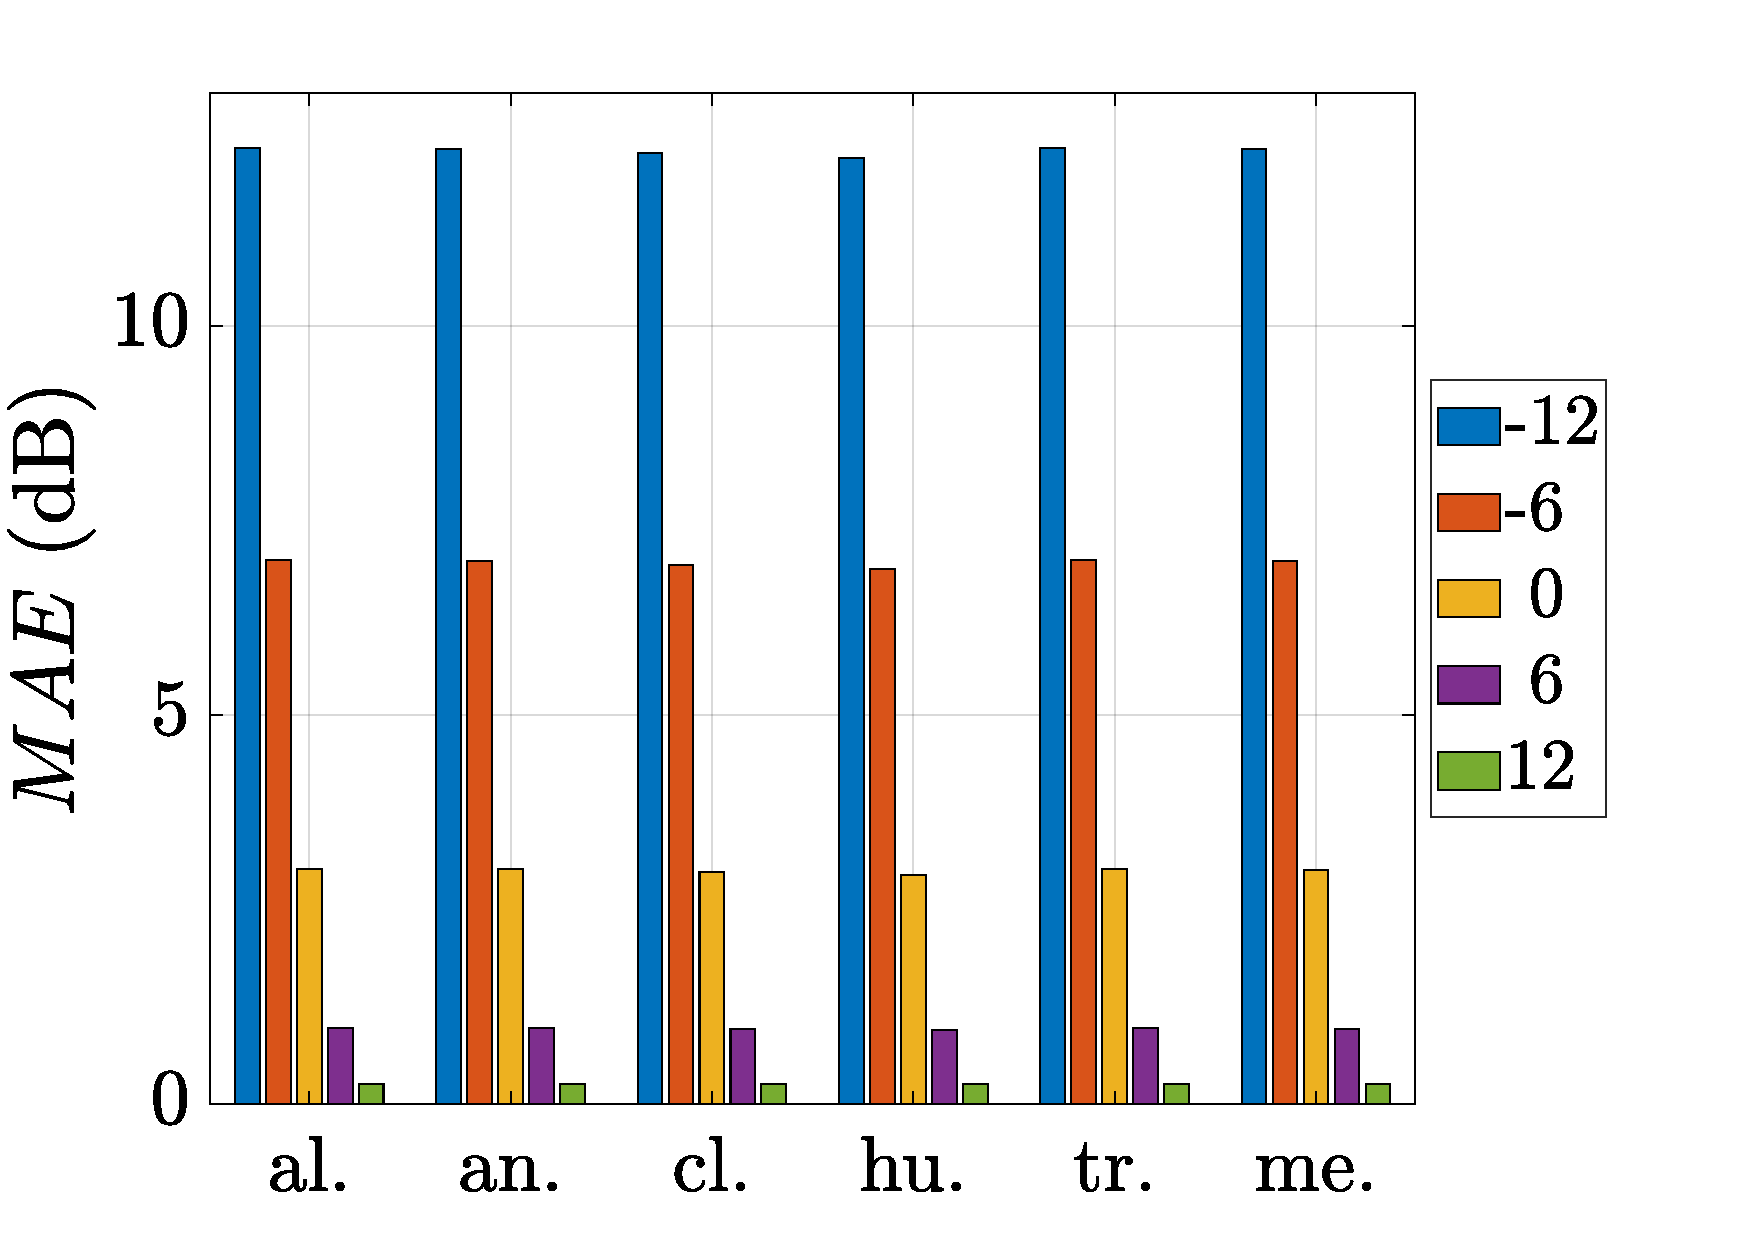
\includegraphics[width=0.7\linewidth]{./figures/resultats/amb_filtre_20k_bar.pdf}
\caption{Erreurs $MAE$ pour chaque sous-corpus et chaque $TIR$ pour l'estimateur filtre passe-bas à la fréquence de coupure $f_c$ = 20 kHz.}
\label{fig:filtre_amb_tir_20k}
\end{figure}

\begin{equation}\label{eq:erreur20k}
\tilde{L}_{eq,tr.,tir} = 10\times \log_{10}\left(10^{L_{eq,tr.,tir}/10}+10^{L_{eq,int.,tir}/10}\right)
\end{equation}


En résumé, le filtre passe-bas avec une fréquence de coupure $f_c$ = 500 Hz est l'approche le plus efficace sur l'ensemble du corpus sans toutefois être la plus performante sur chaque $TIR$. Cette méthode correspond plus à un compromis qui est fait entre l'énergie rejetée dans les $TIR$ négatifs et l'énergie conservée dans les $TIR$ positifs.

\section{Performances de l'estimateur basé sur la NMF}
On résume les erreurs produites par les différentes versions de la NMF d'abord selon l'erreur $MAE_g$ puis, dans un second temps, les erreurs $MAE_{TIR}$ et $MAE$ sont observées pour chaque méthode de NMF proposant les plus faibles erreurs.

\subsection{Erreurs $MAE_g$}

Le nombre de combinaisons de modalités entre les différents facteurs expérimentaux étant important, on résume, dans un premier temps, dans le Tableau \ref{tab:erreur_ambiance_SUP_SEM}, les erreurs $MAE_g$ les plus faibles produites par la NMF SUP et SEM selon chaque valeur de $\beta$ avec les modalités correspondantes. Puis, dans le cas de la NMF IS, l'influence de la représentation de la distance et du type de seuil sont observées dans les Tableaux \ref{tab:erreur_ambiance_IS} et \ref{tab:erreur_ambiance_IS_seuil}.

\begin{table}[h]
\caption{Erreurs $MAE_g$ les plus faibles de la NMF SUP et NMF SEM pour le corpus d'évaluation \textit{Ambiance}, en gras-rouge, l'erreur globale la plus faible.}
\label{tab:erreur_ambiance_SUP_SEM}
\centering
\begin{tabular}{L{2.2cm}C{1.7cm}C{1.2cm}C{1.2cm}C{1.2cm}C{2.5cm}}
\toprule
 & $f_c$ (kHz) & $\beta$ & $w_t$ (s) & $K$ & $MAE_g$ \\ \toprule
\multirow{2}{*}{filtre PB} & 20 & - & - & - & 4,69 ($\pm$ 4,52) \\
 & 0,5 & - & - & - & 2,89 ($\pm$ 2,84) \\
 \midrule
\multirow{3}{*}{NMF SUP} & - & 0 & 2 & 50 & 4,29 ($\pm$ 4,24) \\
 & - & 1 & \textit{all} & 25 & 3,45 ($\pm$ 3,70) \\
 & - & 2 & 2 & 25 & 2,84 ($\pm$ 3,19)  \\
 \midrule
\multirow{3}{*}{\textbf{NMF SEM}} & - & 0 & 2 & 200 & 2,46 ($\pm$ 1,14) \\
 & - & \textbf{1} & \textbf{2} & \textbf{200} & \textbf{\textcolor{red}{2,32 ($\pm$ 1,15)}} \\
 & - & 2 & 2 & 200 & 2,32 ($\pm$ 1,26)\\ \bottomrule
\end{tabular}
\end{table}

La NMF SUP offre des estimations moins bonnes que l'estimateur \textit{baseline} pour $f_c$ = 500 Hz à  $\beta \in \lbrace 0,~1 \rbrace$. L'erreur la plus faible y est atteinte pour $\beta$ = 2 avec une erreur similaire au filtre.
Les 3 NMF SUP obtiennent une erreur minimale pour des dictionnaires différents. Dans le cas de la divergence de KL et EUC, c'est un faible nombre d'éléments qui est requis ($K$ = 25). Dans le cas de la divergence KL, le dictionnaire comprend un faible nombre d'éléments avec $w_t = all$, qui correspond au cas où le dictionnaire contient des enveloppes spectrales. La NMF SUP étant plus contrainte dans son fonctionnement, puisqu'elle doit avec un dictionnaire fixe \textit{trafic} s'adapter aux différents sous-corpus, avoir un dictionnaire qui généralise au mieux les spectres liés au trafic. Le dictionnaire de la NMF SUP avec $\beta \in \lbrace 0,~2 \rbrace$ est basé sur une description fine du corpus d'apprentissage ($w_t = 0,5$ s). Dans le cas de la distance EUC, étant sensible aux fortes variations d'énergie spectrale entre $\mathbf{V}_{fn}$ et $\left[\mathbf{WH}\right]_{fn}$, elle privilégie un dictionnaire construit sur une description fine afin de mieux prendre en compte les variations spectrales de la source \textit{trafic}.

La NMF SEM offre des erreurs plus faibles que l'estimateur \textit{baseline} pour les 3 valeurs de $\beta$ avec des écarts-types réduits. Dans les 3 cas, le dictionnaire est basé sur les mêmes modalités avec ici un grand nombre d'éléments ($K$ = 200).
La différence entre la NMF SEM et SUP réside dans la présence du dictionnaire libre $\mathbf{W_r}$ dans la NMF SEM qui permet plus d'adaptabilité (deux exemples de la forme des matrices $\mathbf{W_r}$ sont présentés en Figure \ref{fig:Y_ambiance}).\\

La NMF IS étant une forme de NMF proposée pour ces travaux, plusieurs pistes sont explorées afin de trouver une configuration optimale selon le choix de la représentation de la distance $D_{\theta}$ ou le type de seuillage. En considérant ces facteurs expérimentaux indépendants, il est possible de regarder leur influence séparément et ainsi éviter de calculer l'ensemble des combinaisons de modalités. Dans un premier temps, la représentation de la distance $D_{\theta}$, linéaire ou exprimée à travers une fonction sigmoïde, est observée dans le Tableau \ref{tab:erreur_ambiance_IS} selon un seuillage dur.

\begin{table}[h]
\centering
\caption{Erreurs $MAE_g$ les plus faibles de la NMF IS pour le corpus d'évaluation \textit{Ambiance} selon la représentation linéaire ou sigmoïde de la distance $D_{\theta}$.}
\label{tab:erreur_ambiance_IS}
\begin{tabular}{C{1.2cm}C{1.2cm}C{1.2cm}C{2.5cm}C{1.2cm}C{2.5cm}}
\toprule
$\beta$ & $w_t$ & $K$ & \textbf{représentation} & $t_h$ & $MAE_g$ \\ \toprule
\multirow{2}{*}{0} & 500 & 200 & linéaire & 0,47 & 2,26 ($\pm$ 2,15) \\
 & 500 & 200 & sigmoïde & 0,61 & 2,25 ($\pm$ 2,37) \\ \midrule
\multirow{2}{*}{\textbf{1}} & \textbf{500} & \textbf{200} & \textbf{linéaire} & \textbf{0,41} & \textbf{\textcolor{red}{2,14 ($\pm$ 2,10)}} \\
 & 500 & 200 & sigmoïde & 0,60 & 2,14 ($\pm$ 2,14) \\ \midrule
\multirow{2}{*}{2} & 500 & 200 & linéaire & 0,36 & 2,29 ($\pm$ 2,40)\\
 & 500 & 200 & sigmoïde &  0,59 & 2,26 ($\pm$ 2,43)  \\
\bottomrule
\end{tabular}
\end{table}

Dans un premier temps, on remarque, comme pour la NMF SEM, que la méthode privilégie un nombre d'éléments dans le dictionnaire important ($K$ = 200). De plus, le choix de la représentation de $D_{\theta}$ n'influe pas sur la formation du dictionnaire puisque $w_t$ et $K$ restent constants.
L'erreur $MAE_g$ selon la représentation de $D_{\theta}$ est très peu influencée : les erreurs restent équivalentes, seuls les seuils doivent être adaptés. La fonction sigmoïde déformant $D_{\theta}$, les valeurs des seuils doivent être réhaussées. L'impact de cette fonction sur l'erreur $MAE_g$ étant très faible par rapport à la représentation linéaire, c'est cette dernière qui est donc choisie pour la suite.

L'allure moyenne de $D_{\theta}$ pour chaque valeur du $TIR$ avec $w_t$ = 0,5 s, $K$ = 200 et $\beta$ = 1 avec une représentation linéaire est alors résumée en Figure \ref{fig:dist_TIR}. Pour un seuil fixé à $t_h$ = 0,41, le nombre d'éléments considéré dans $\mathbf{W}_{trafic}$ est donc variable. Pour les $TIR$ négatifs, les distance $D_{\theta}$ sont plus faibles, traduisant la déviation des spectres initiaux pour des spectres liés aux classes \textit{interférantes}. À $TIR$ = -12 dB, c'est 106 éléments en moyenne qui sont considérés comme appartenant à la classe \textit{trafic}. Plus le $TIR$ augmente et plus ces distances augmentent, puisque le trafic devient la classe de son prédominante. À $TIR$ = 12 dB, c'est alors 181 éléments qui sont inclus dans le dictionnaire \textit{trafic}.

\begin{figure}[h!]
\centering
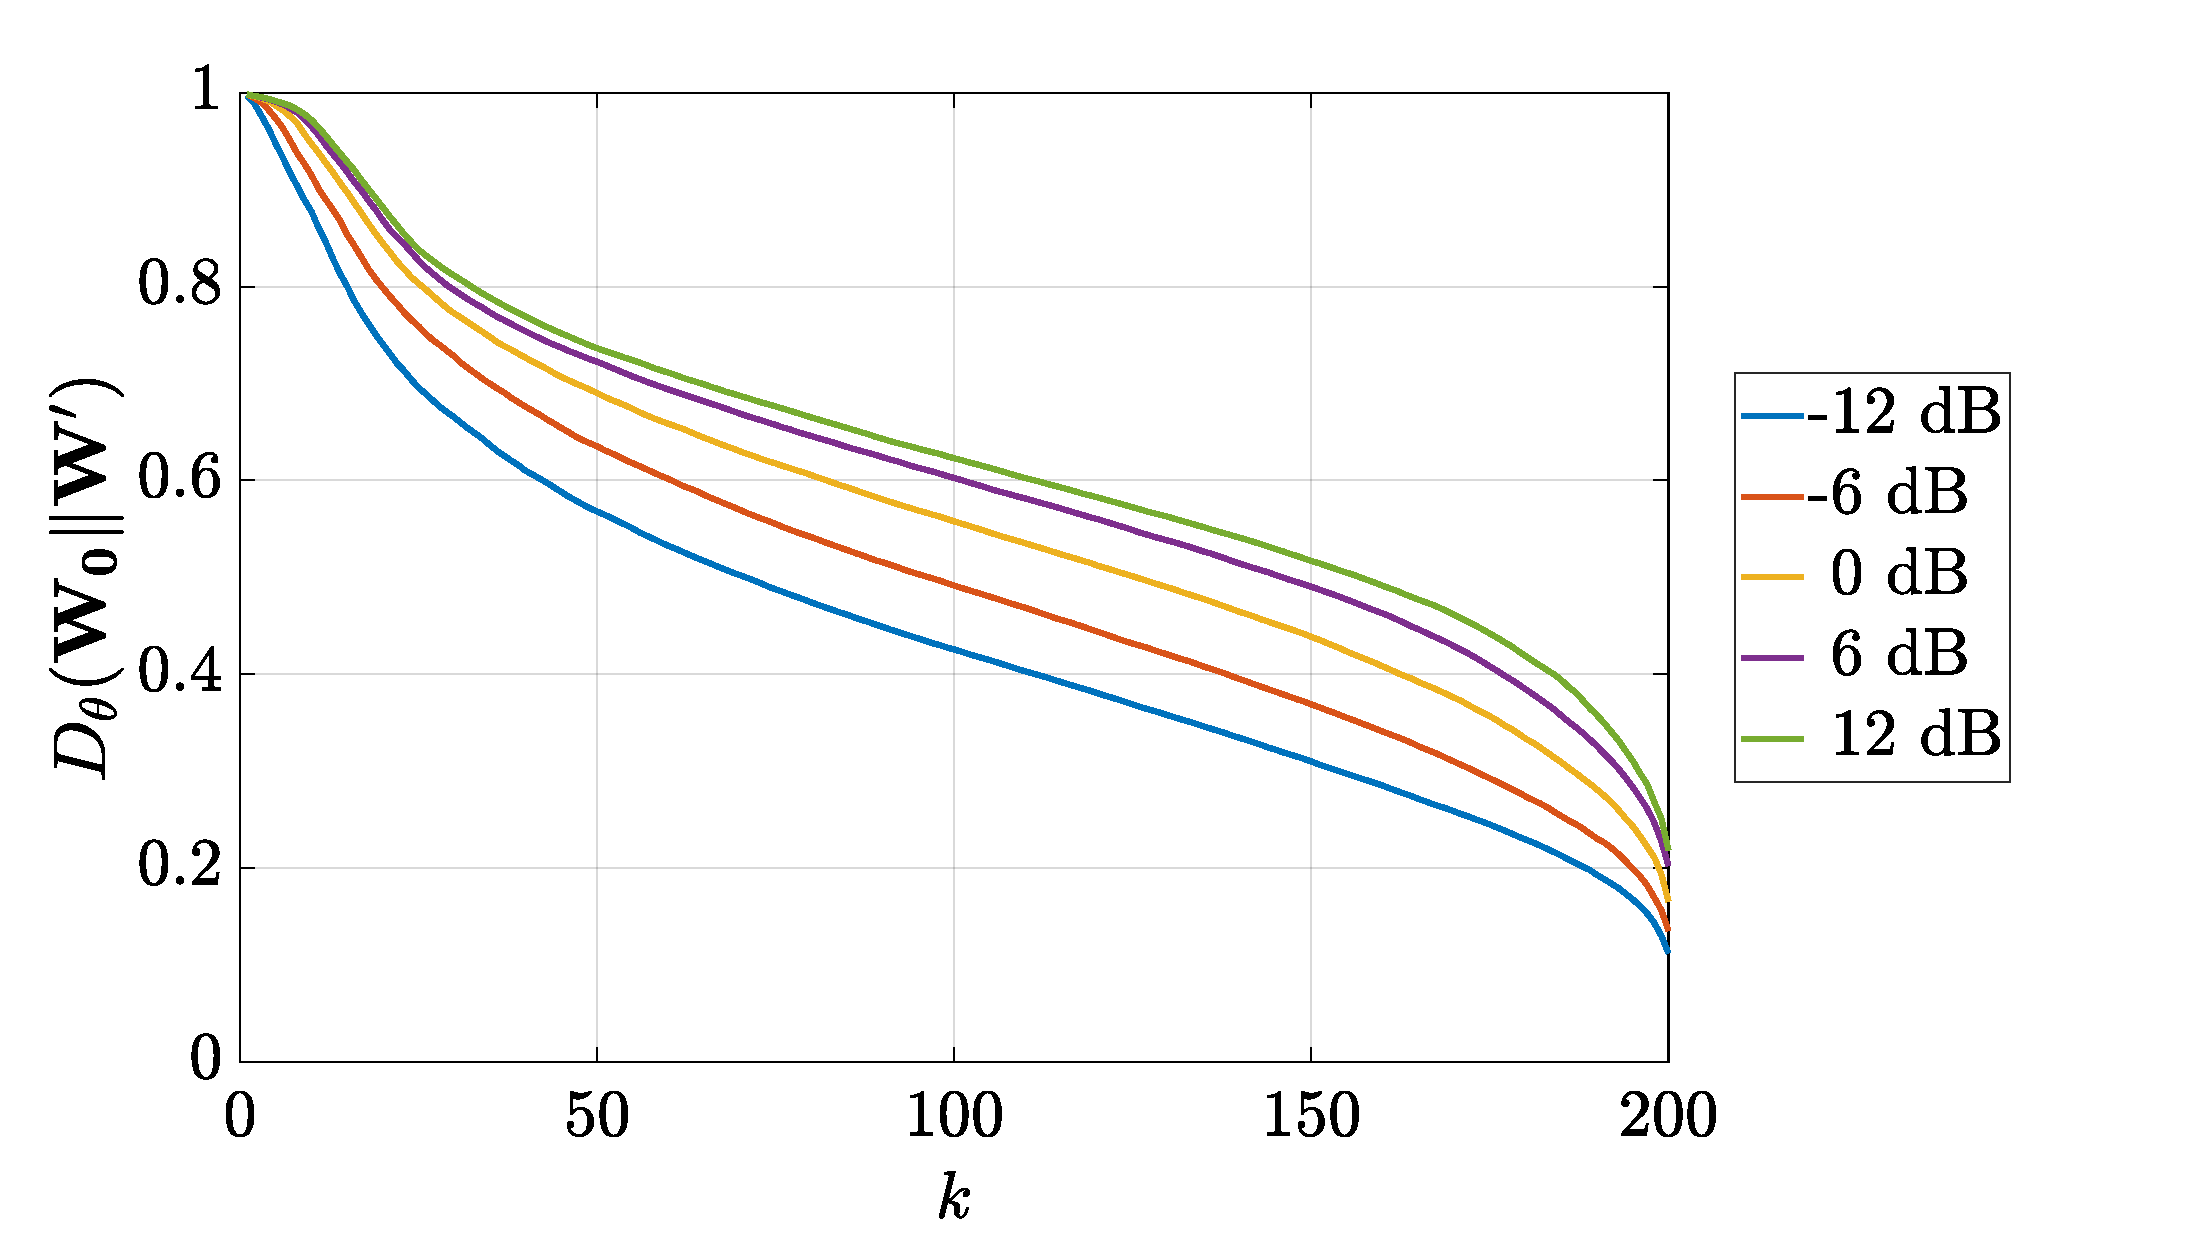
\includegraphics[width=.8\linewidth]{./figures/resultats/dist_TIR.pdf}
\caption{Distances moyennes $D_{\theta}(\mathbf{W_0} \Vert \mathbf{W'})$ triées par ordre décroissant pour chaque $TIR$,  obtenues pour $w_t$ = 0,5 s, $K$ = 200 et $\beta$ = 1.}
\label{fig:dist_TIR}
\end{figure}


À partir de la représentation de $D_{\theta}$, l'influence de la technique du seuillage sur les erreurs $MAE_g$ est présentée dans le Tableau \ref{tab:erreur_ambiance_IS_seuil} pour chaque valeur de $\beta$. On rappelle que le seuillage dur définit les éléments dans le dictionnaire $\mathbf{W'}$ selon un classement binaire alors que le seuillage \textit{firm} considère deux valeurs de seuil où les éléments dont la distance $D_{\theta}$ est située entre ces valeurs sont pondérés.

\begin{table}[h]
\centering
\caption{Erreurs $MAE_g$ les plus faibles de la NMF IS pour le corpus d'évaluation \textit{Ambiance} selon un seuillage dur ou \textit{firm}.}
\label{tab:erreur_ambiance_IS_seuil}
\begin{tabular}{C{1.2cm}C{1.2cm}C{1.2cm}C{1.2cm}C{1.2cm}C{1.2cm}C{2.5cm}}
\toprule
$\beta$ & $w_t$ & $K$ & $t_h$ & $t_{f,1}$ & $t_{f_2}$ & $MAE$ \\ \toprule
\multirow{2}{*}{0} & 500 & 200 & 0,47 & - & - & 2,26 ($\pm$ 2,15) \\
 & 500 & 200 & - & 0,44 & 0,50 & 2,25 ($\pm$ 2,14)  \\ \midrule
\multirow{2}{*}{\textbf{1}} & 500 & 200 & 0,41 & - & - & 2,14 ($\pm$ 2,10) \\
 & \textbf{500} & \textbf{200} & - & \textbf{0,39} & \textbf{0,42} & \textbf{\textcolor{red}{2,13 ($\pm$ 2,16)}}  \\ \midrule
\multirow{2}{*}{2} & 500 & 200 &  0,36 & - & - & 2,29 ($\pm$ 2,40)\\
 & 500 & 200 & - & 0,23 & 0,48 & 2,21 ($\pm$ 2,49)  \\
 \bottomrule
\end{tabular}
\end{table}


Là encore, le dictionnaire optimal reste le même et n'est pas influencé par le choix de la technique du seuillage. On constate que les valeurs de seuils $t_{f,1}$ et $t_{f,2}$ encadrent la valeur du seuil dur $t_h$. Si cet encadrement est large pour $\beta = 2$, pour $\beta \in \lbrace 0,~1 \rbrace$ cet encadrement est plus restreint. Cela correspond, pour $\beta$ = 1, à considérer dans $\mathbf{W}_{trafic}$, en moyenne 145 ($\pm$ 32) éléments issus directement de $\mathbf{W'}$ et à y inclure 8 ($\pm$ 2) éléments pondéré selon la relation \ref{eq:seuillageFirm_def}. Sur l'ensemble des cas, l'apport du seuillage \textit{firm} est quasi nul par rapport au seuillage dur. En conséquence, puisque l'influence du seuillage \textit{firm} reste là aussi très faible, en vue de simplifier l'étude, on ne considère finalement que le cas d'une NMF IS avec une représentation linéaire de $D_{\theta}$ et un seuillage dur. \\

De ces premiers résultats, moyennés sur l'ensemble du corpus d'évaluation, on retient donc les combinaisons de modalités les plus performantes pour chaque NMF :

\begin{itemize}
\item NMF SUP avec $\beta$ = 2, $K$ = 25, et $w_t$ = 2 s,
\item NMF SEM avec $\beta$ = 1, $K$ = 200, et $w_t$ = 2 s,
\item NMF IS avec $\beta$ = 1, $K$ = 200, $w_t$ = 0,5 s et $t_h$ = 0,41.\\
\end{itemize}

Avant d'observer leur erreurs $MAE_{TIR}$ et $MAE$, l'influence de la forme du dictionnaire sur les erreurs $MAE_g$ sont observées.

\subsection{Influence des facteurs expérimentaux $w_t$ et $K$}

\begin{figure}[h!]
\centering
\subfigure[Influence du facteur expérimental $w_t$ sur les 3 versions optimales de NMF.]{%
\label{fig:influence_wt}%
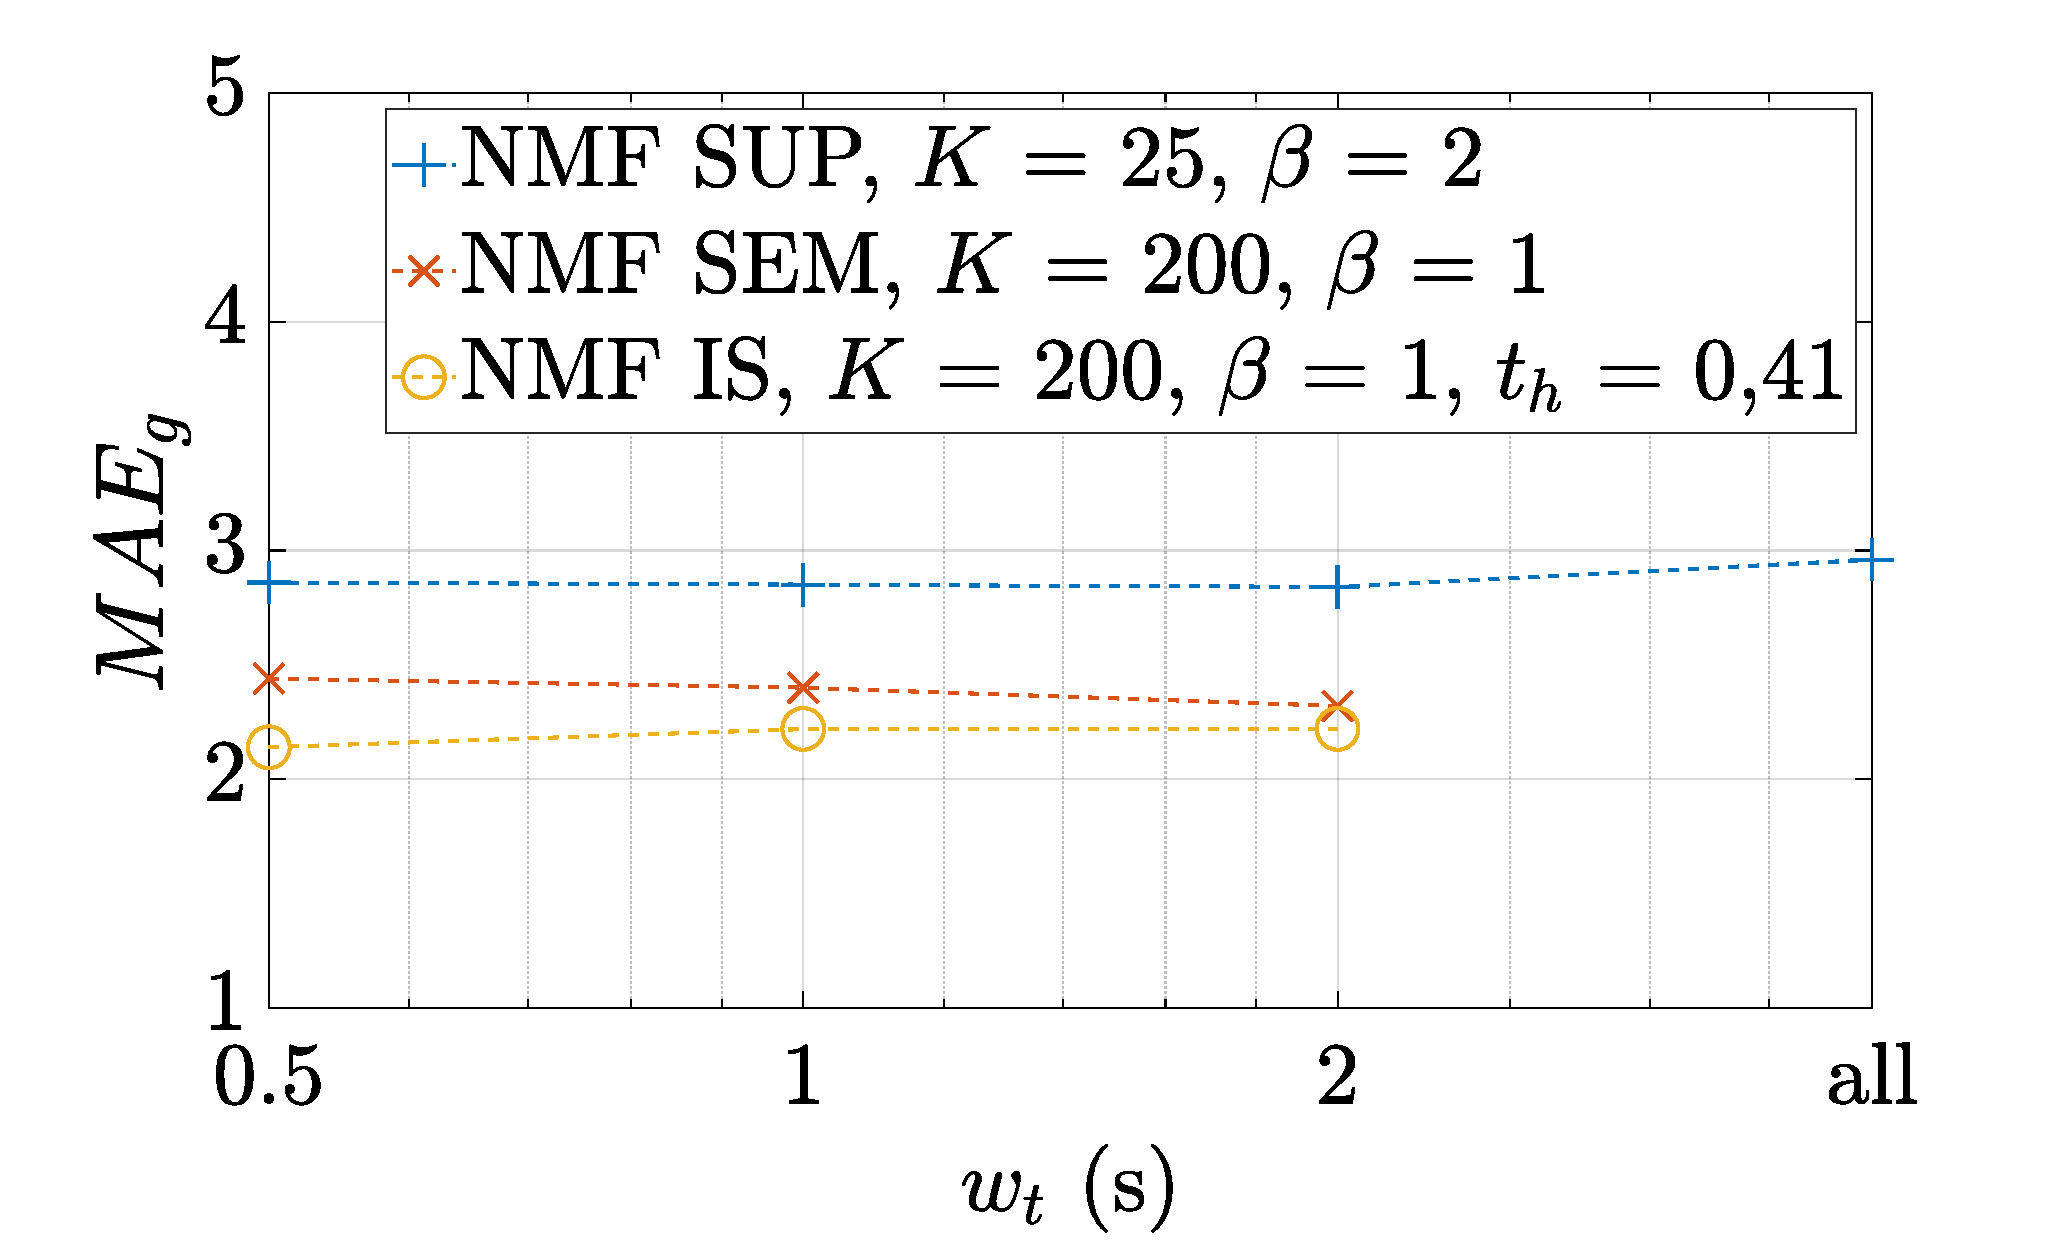
\includegraphics[width=.45\linewidth]{./figures/resultats/influence_wt.pdf}}%
\qquad
\subfigure[Influence du facteur expérimental $K$ sur les 3 versions optimales de NMF.]{%
\label{fig:influence_K}%
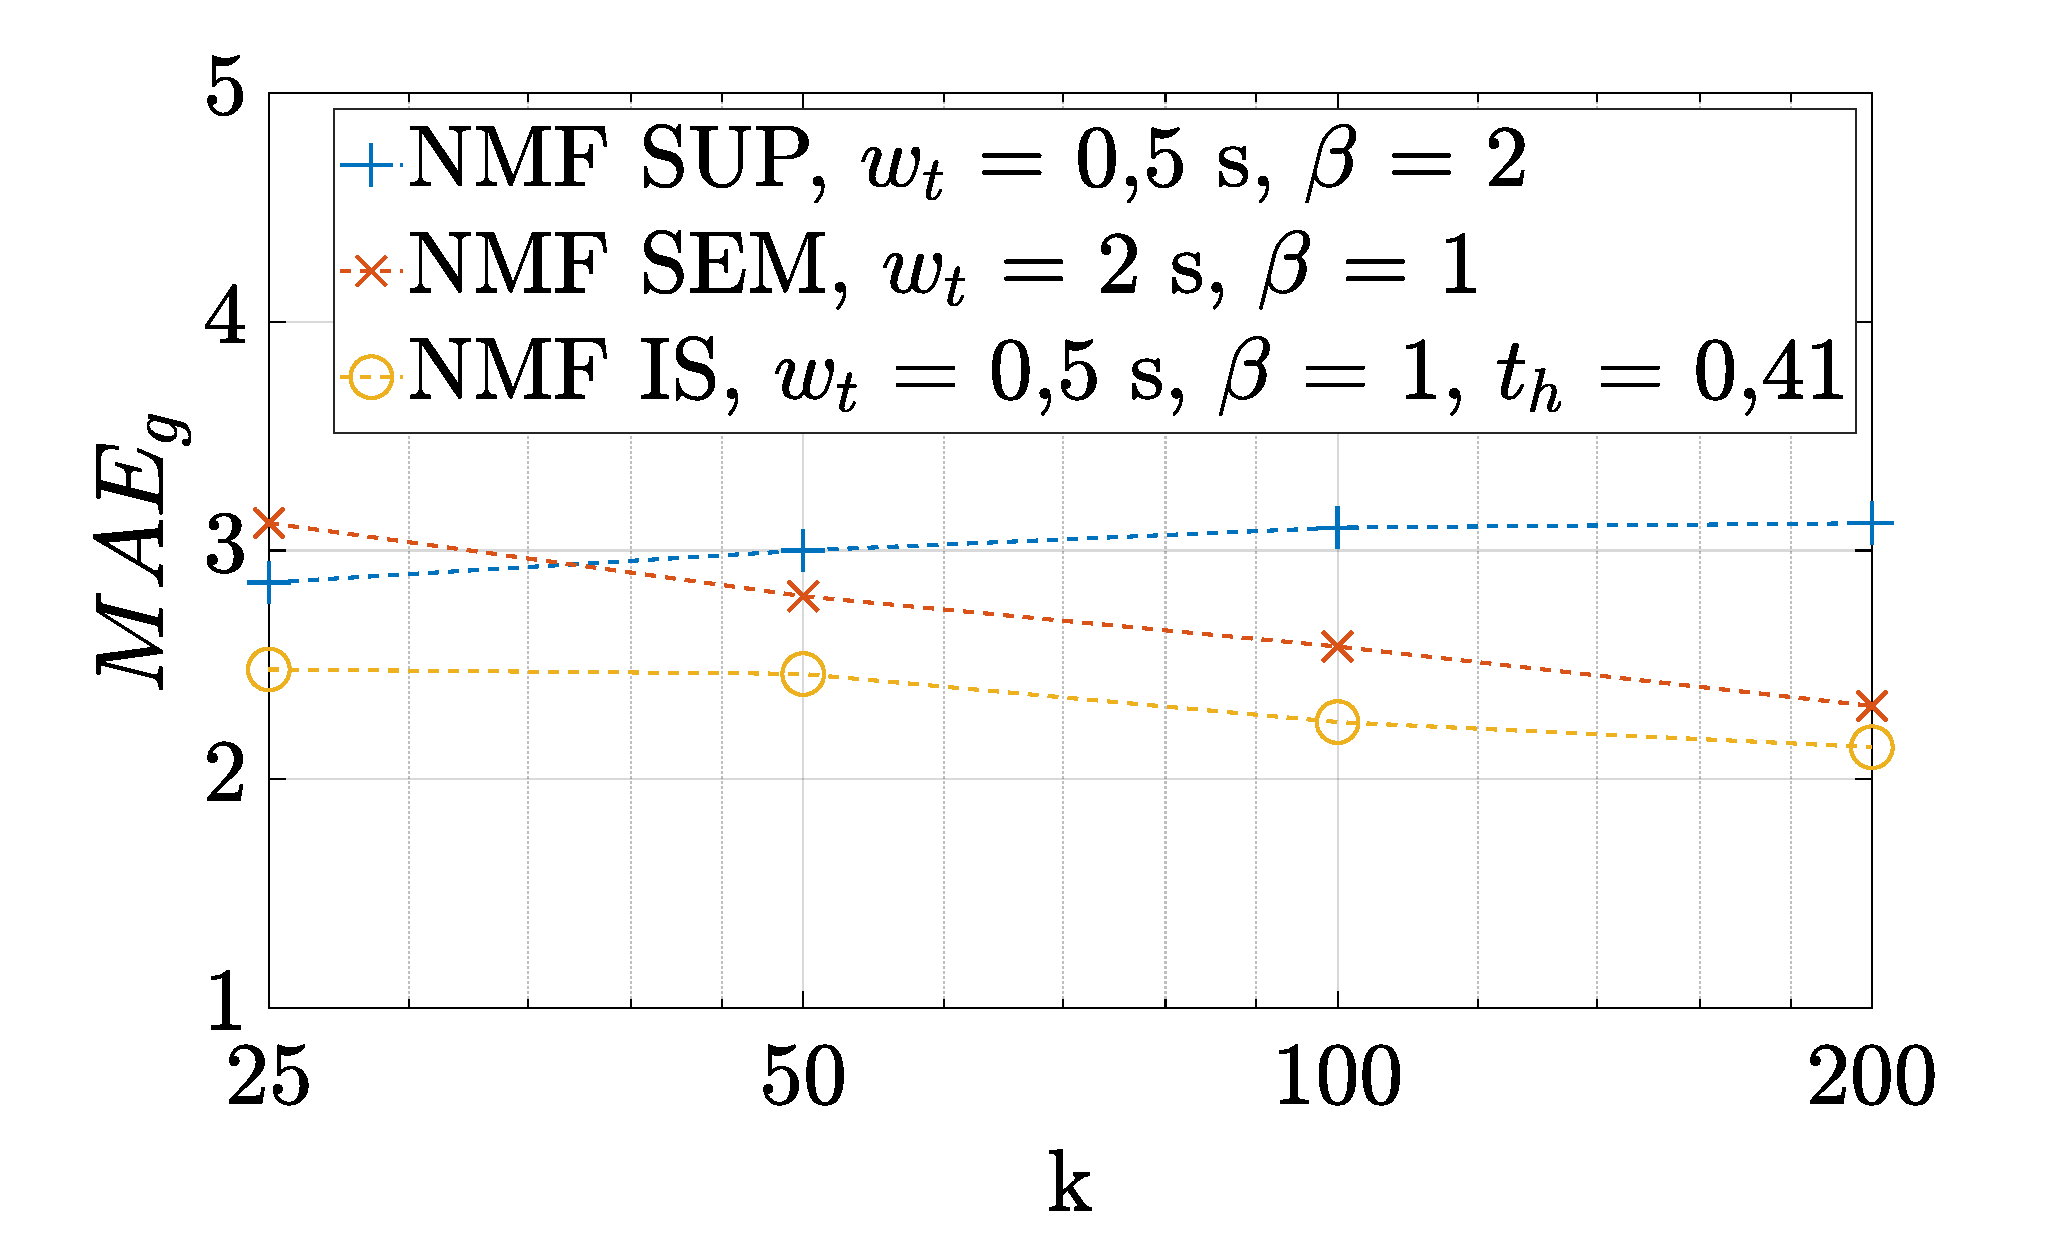
\includegraphics[width=.45\linewidth]{./figures/resultats/influence_K.pdf}}%
\caption{Influence de la forme du dictionnaire pour les 3 NMF retenues.}
\label{fig:influence_dict}
\end{figure}


Si le choix de la méthode et de la valeur de $\beta$ sont des facteurs expérimentaux prédominant dans les erreurs produites, l'influence de la forme du dictionnaire est à connaitre également. Pour cela, selon les 3 formes de NMF retenues, l'influence de la taille de la fenêtre de découpage $w_t$ est observé en Figure \ref{fig:influence_wt}. Pour la NMF SUP, ayant un faible nombre d'éléments dans $\mathbf{W}$ le cas où $w_t$ = \textit{all} peut être observé, alors que pour la NMF SEM et IS, il n'est pas possible de l'observer puisque le nombre d'éléments ($K$ = 200) est plus élevé que le nombre de fichiers audio disponibles.
L'influence du facteur $w_t$ est très faible sur l'erreur de reconstruction du signal \textit{trafic} notamment pour $w_t \in \lbrace 0.5,~1,~2\rbrace$, pour le 3 formes de NMF. Pour la NMF IS, son influence est vouée à être réduite puisque le dictionnaire est mis à jour. On ne constate qu'un impact réel que pour le cas de la NMF SUP avec $w_t = all$ qui correspond au cas où les enveloppes des spectres \textit{trafic} sont considérées dans le dictionnaire. L'utilisation de l'algorithme $K$-means et la représentation en bandes de tiers d'octave dans la construction du dictionnaire peut avoir réduit l'impact de ce facteur expérimental.
La Figure \ref{fig:influence_K} montre de manière synthétique l'évolution des erreurs $MAE_g$ selon le nombre d'éléments $K$ contenu dans le dictionnaire.
Pour les 3 NMF, ce facteur est un paramètre plus influant que $w_t$.
La NMF SUP privilégie un dictionnaire composé d'un faible nombre d'éléments. Ce comportement se justifie par le fonctionnement de la NMF SUP en elle même : contrainte avec un seul dictionnaire fixe à s'adapter à l'ensemble des cas rencontrés, cette méthode privilégie les dictionnaires composé d'une quantité d'information réduite, plus générique afin d'être le plus généralisable possible.
À l'inverse, dans le cas de la NMF IS et SEM, l'erreur diminue avec l'augmentation de $K$. Ces deux méthodes gagnent donc à être composées d'un grand nombre d'éléments pour mieux décrire la source sonore.
Dans le cas de la NMF IS cela se comprend d'autant plus qu'avec un nombre suffisant d'éléments dans le dictionnaire $\mathbf{W'}$, celui-ci permet une description plus fine et mieux adaptée à la scène.

\subsection{Influence de l'initialisation de la NMF IS}

Le principe de la NMF IS est d'apprendre un dictionnaire $\mathbf{W_0}$ composé de spectres de la source sonore d'intérêt pour ensuite le mettre à jour à chaque itération. La sélection des éléments liés à la source dans $\mathbf{W'}$ se fait alors par comparaison entre le dictionnaire initial $\mathbf{W_0}$ et final $\mathbf{W'}$. Le choix d'utiliser un dictionnaire appris à pour but d'orienter les mises à jour des matrices vers la source d'intérêt. Pour visualiser l'impact de cette orientation, on compare le cas de la NMF IS optimale ($K$ = 200, $w_t$ = 0,5 s, $\beta$ = 1) avec une initialisation faite par $\mathbf{W_0}$ et avec valeurs aléatoires. Dans ce dernier cas, après 100 itérations, le dictionnaire obtenu $\mathbf{W'}$ est alors comparé à $\mathbf{W_0}$. Le Tableau \ref{tab:erreur_ambiance_IS_initialisation} résume les erreurs $MAE_g$ obtenues avec le seuil $t_h$ = 0,41 et pour le seuil optimal de la NMF IS initiée avec des valeurs aléatoires.

\begin{table}[h]
\centering
\caption{Erreurs $MAE_g$ les plus faibles de la NMF IS pour le corpus d'évaluation \textit{Ambiance} selon l'initialisation du dictionnaire. En ligne 1 et 3, le seuil est celui permettant d'obtenir l'erreur la plus faible, en ligne 2, le seuil correspond à celui obtenu avec une initialisation par $\mathbf{W_0}$ mais sur une NMF IS initialisée par des valeurs aléatoires.}
\label{tab:erreur_ambiance_IS_initialisation}
\begin{tabular}{C{3.5cm}C{1.2cm}C{1.2cm}C{1.2cm}C{1.2cm}C{2.5cm}}
\toprule
\textbf{initialisation} & $\beta$ & $w_t$ & $K$ & $t_h$ & $MAE_g$ \\ \toprule
$\mathbf{W_0}$ & 1 & 500 & 200 & 0,41 & 2,14 ($\pm$ 2,10) \\
 \rowcolor[HTML]{C0C0C0}
valeurs aléatoire & 1 & 500 & 200 & 0,41 & 5,21 ($\pm$ 1,31) \\
valeurs aléatoire & 1 & 500 & 200 & 0,23 & 2,45 ($\pm$ 2,25) \\
 \bottomrule
\end{tabular}
\end{table}

L'initialisation par des valeurs aléatoires génère des erreurs supérieures à la NMF IS initiée avec $\mathbf{W_0}$. La recherche d'une erreur minimale nécessite de diminuer la valeur seuil correspondante à $t_h'$ = 0,23. Un seuil plus faible signifie que la méthode considère un plus grand nombre d'éléments dans le dictionnaire. La Figure \ref{fig:distRand} résume les distances $D_{\theta}$ moyennes à chaque $TIR$ pour une initialisation aléatoire.
Les valeurs de $D_{\theta}$ sont plus faibles traduisant une disparité plus forte entre $\mathbf{W_0}$ et $\mathbf{W'}$. La dispersion des distance $D_{\theta}$ par $TIR$ est également plus faible que dans le cas où $\mathbf{W_0}$ est utilisé (voir Figure \ref{fig:dist_TIR}). On constate également qu'aucune valeur de $D_{\theta}$ n'atteint une similarité de 1. Sans l'initialisation, le dictionnaire mis à jour s'éloigne donc plus de la source \textit{trafic} générant des erreurs plus élevées. Utiliser $\mathbf{W_0}$ à la première itération a donc un impact réel et permet de mieux focaliser les mises à jour du dictionnaire sur la source \textit{trafic} et ainsi de mieux reconstruire cette source sonore.


\begin{figure}[h]
\centering
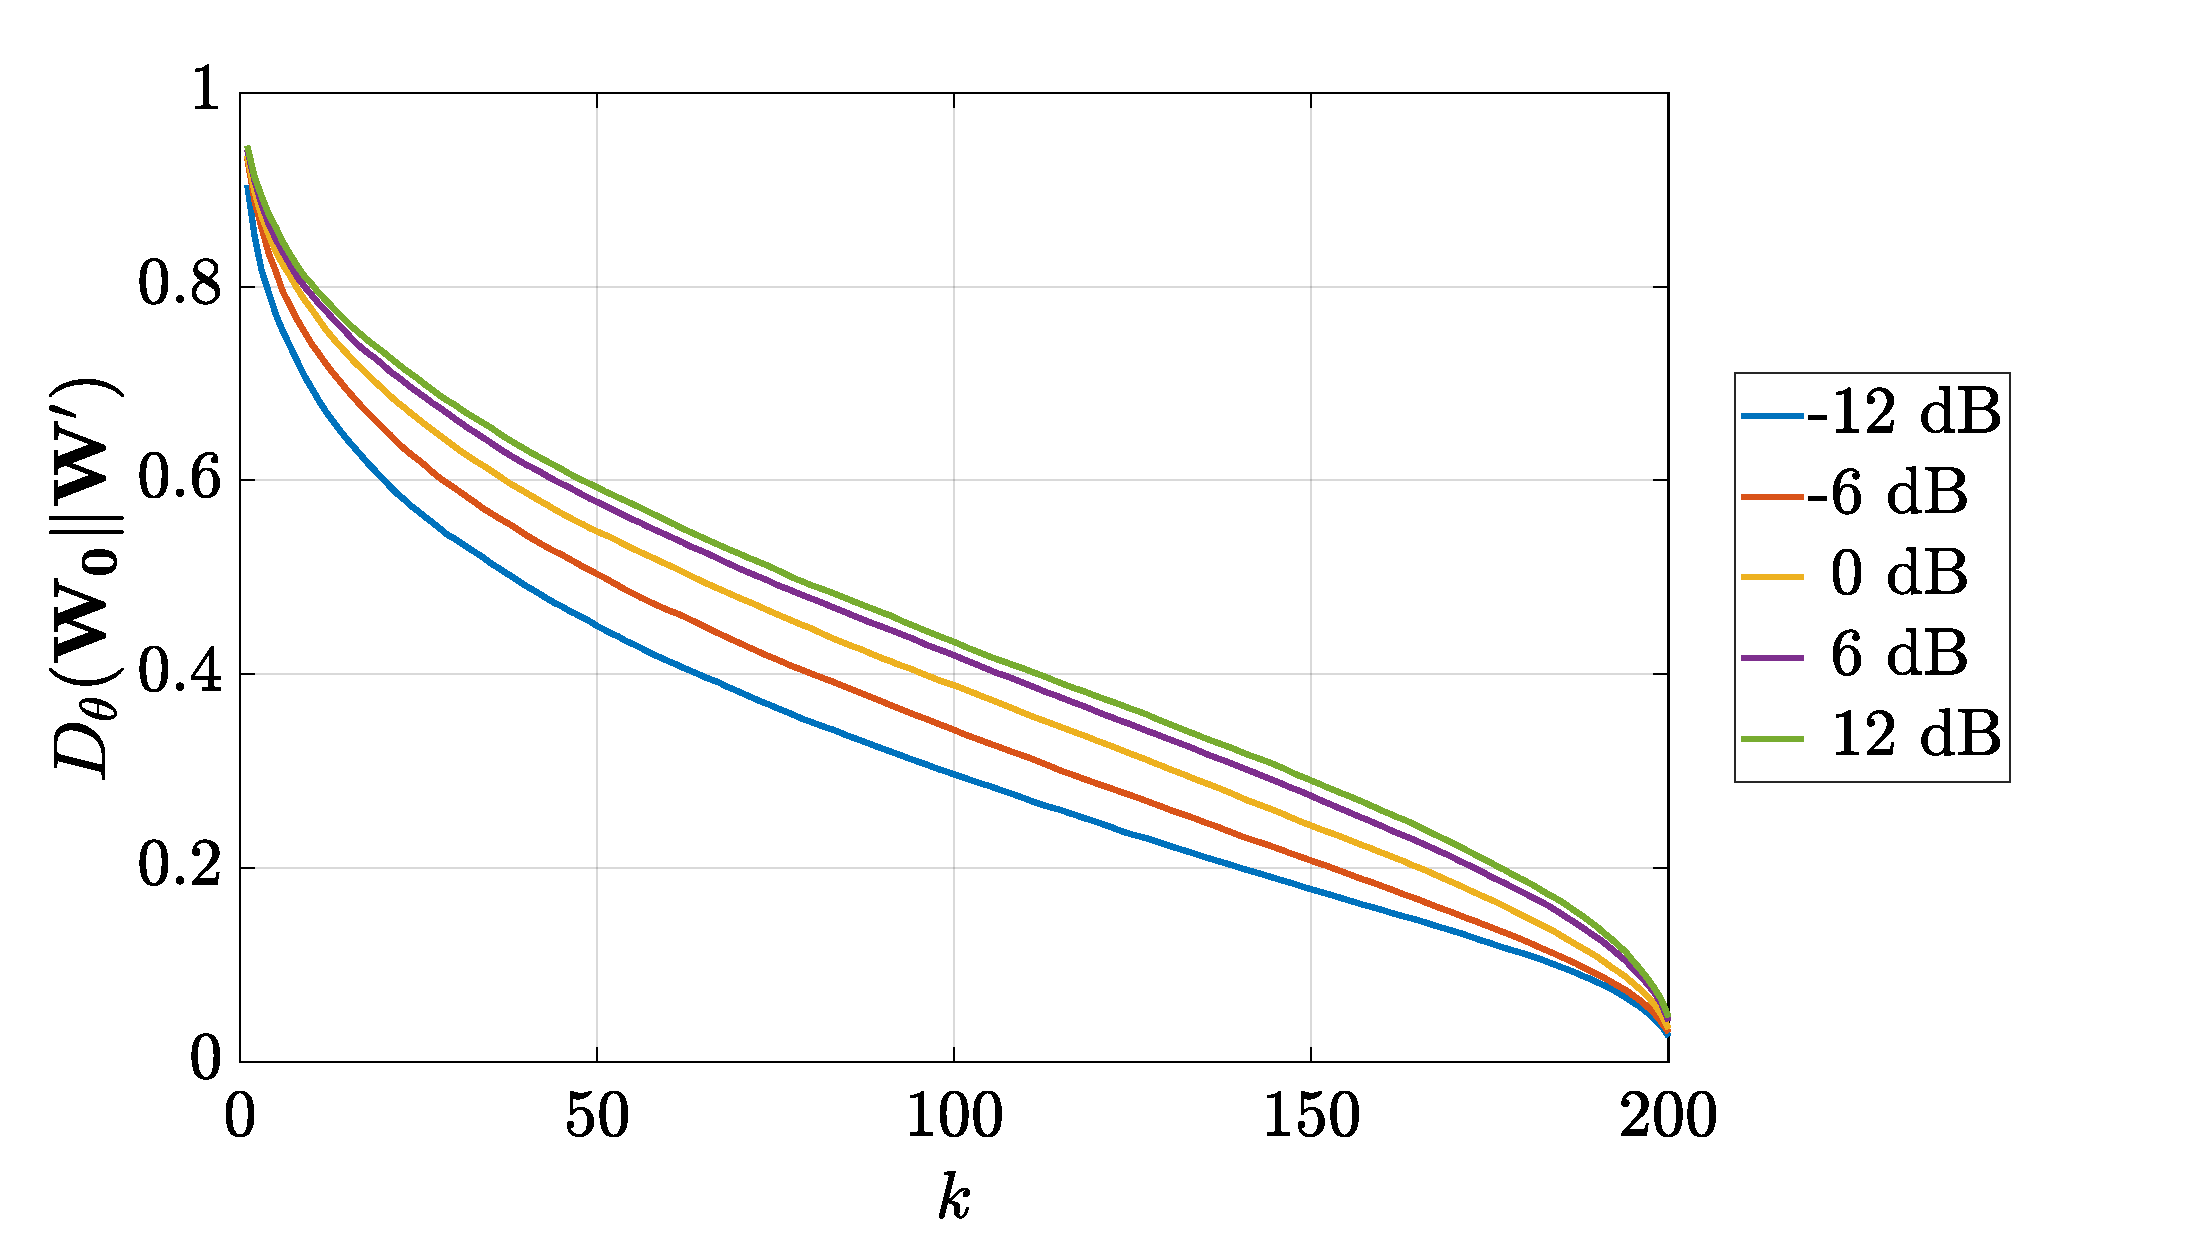
\includegraphics[width=.8\linewidth]{./figures/resultats/distRAND_TIR.pdf}
\caption{Distances moyennes $D_{\theta}(\mathbf{W_0} \Vert \mathbf{W'})$ triées par ordre décroissant pour chaque $TIR$,  obtenues pour $w_t$ = 0,5 s, $K$ = 200 et $\beta$ = 1 pour un dictionnaire initialisé par des valeurs aléatoires.}
\label{fig:distRand}
\end{figure}

\subsection{Erreurs $MAE_{TIR}$ et fonctions de coût}

\begin{figure}[h!]
\centering
\subfigure[Fonction de coût moyennée sur l'intégralité du corpus d'évaluation \textit{Ambiance}]{%
\label{fig:amb_cost}%
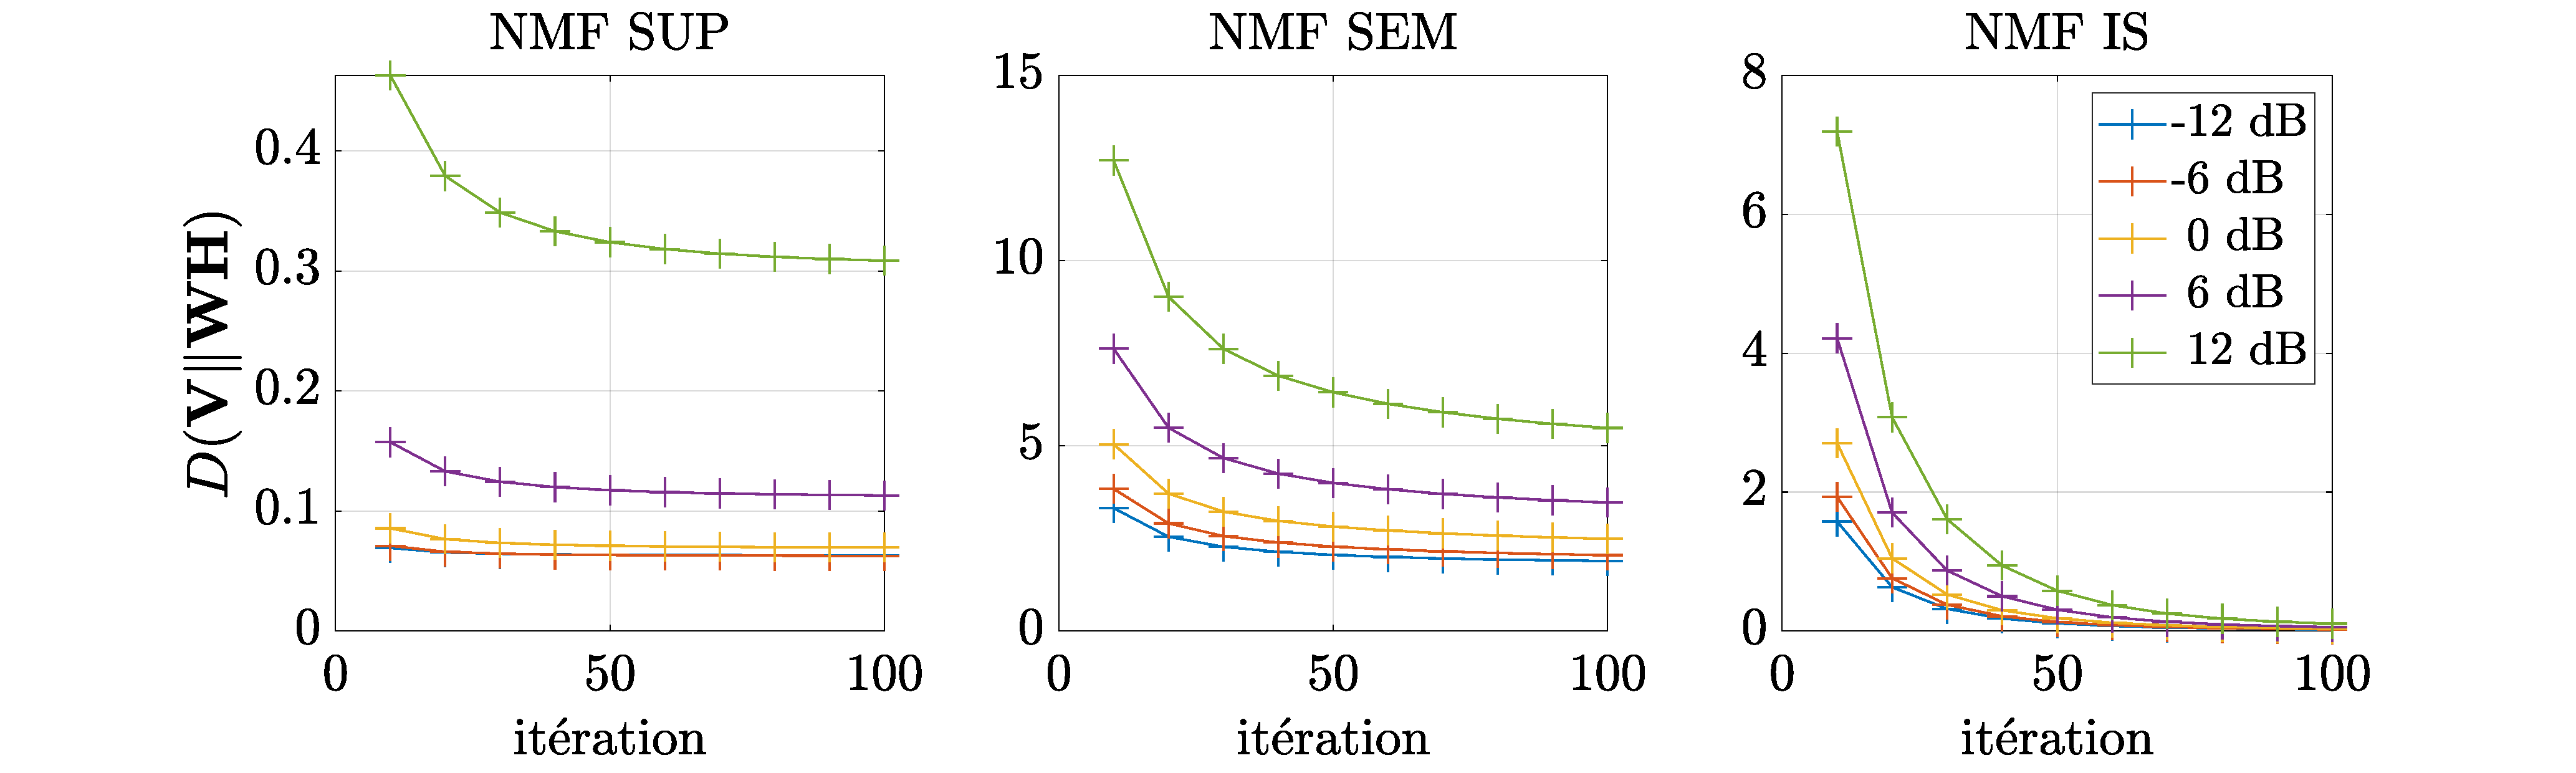
\includegraphics[width=0.45\linewidth]{./figures/resultats/ambiance_cost.pdf}}%
\qquad
\subfigure[Erreur $MAE_g$ moyennée sur l'intégralité du corpus d'évaluation \textit{Ambiance}]{%
\label{fig:amb_mae}%
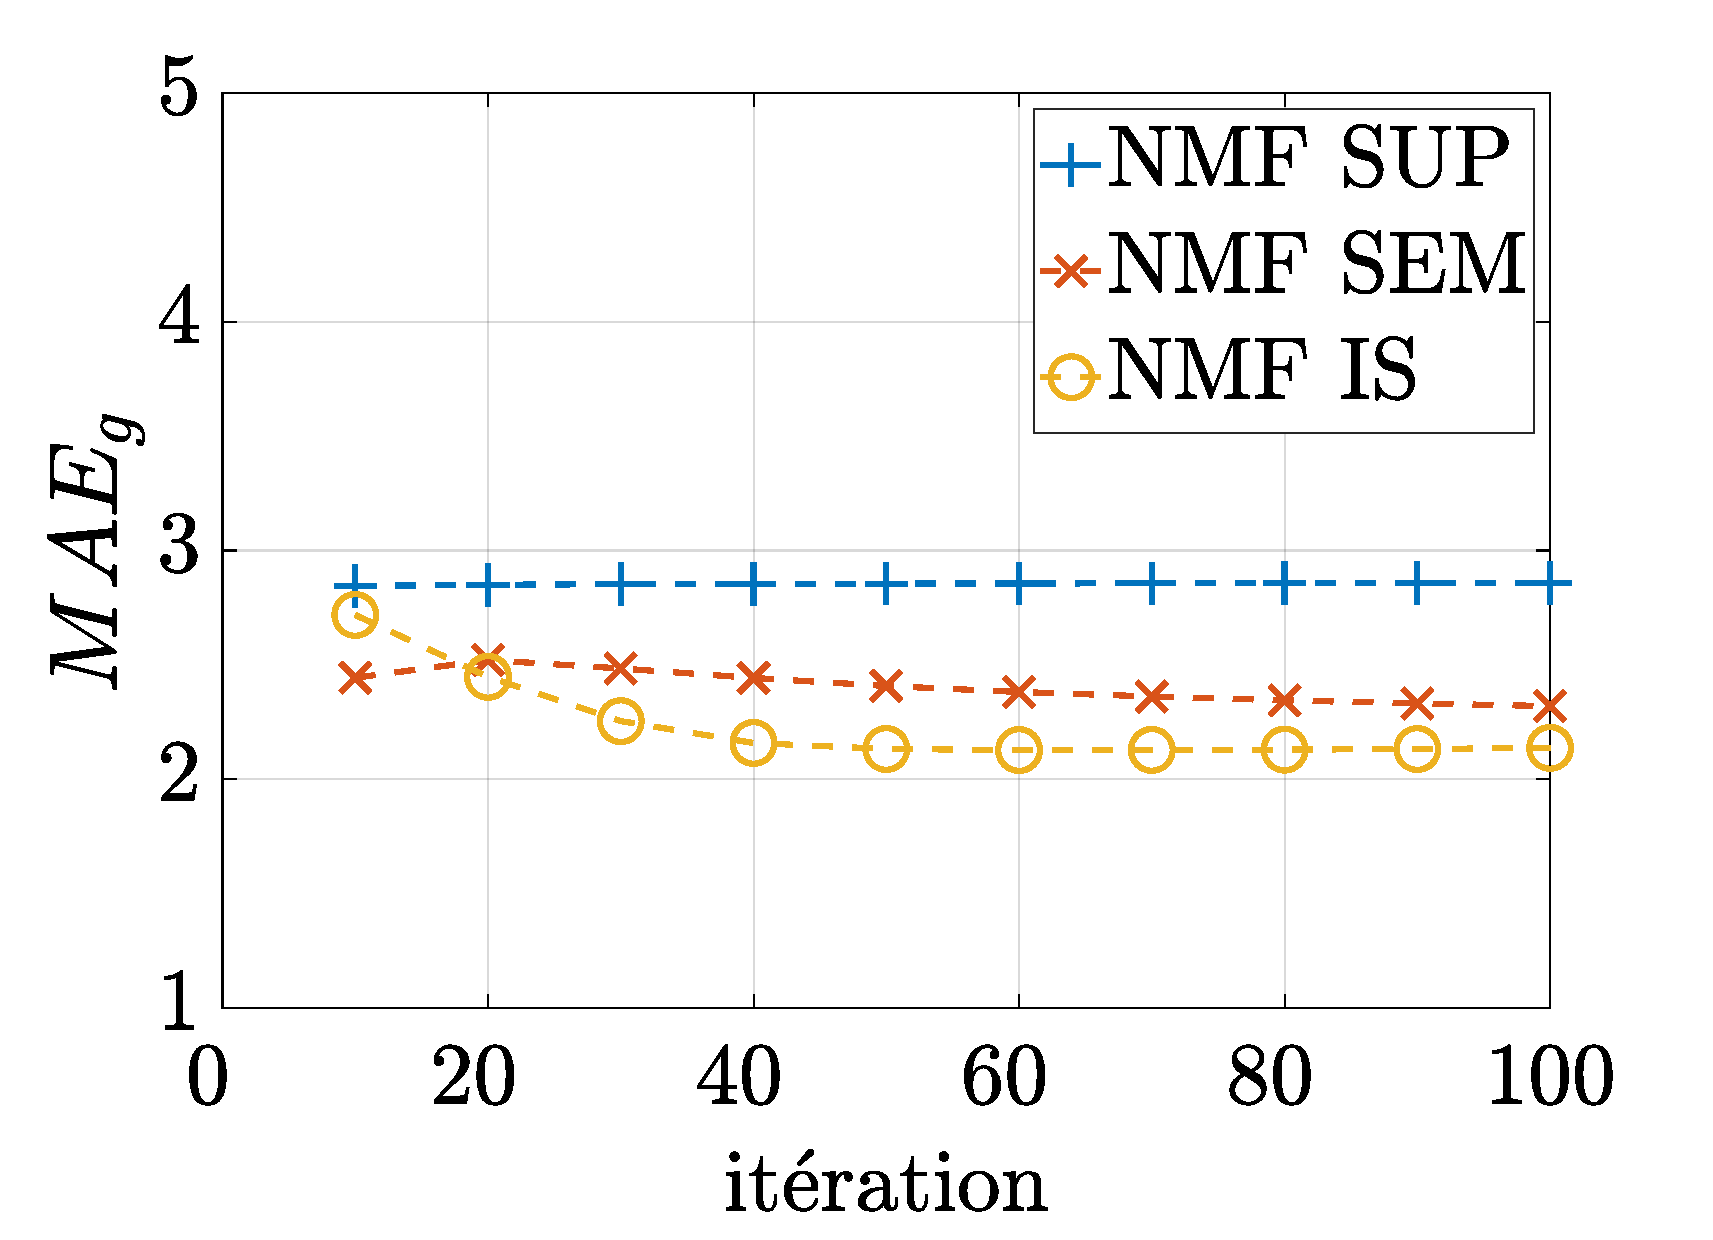
\includegraphics[width=0.45\linewidth]{./figures/resultats/ambiance_mae.pdf}}%
\caption{Evolution de la fonctions de coût $D(\mathbf{V}\Vert \mathbf{WH})$ et de l'erreur $MAE_g$ moyennes pour les combinaisons optimales des NMF SUP, SEM et IS.}
\label{fig:amb_cost_mae}
\end{figure}

La NMF est réalisée en cherchant à minimiser la fonction de coût $D(\mathbf{V}\Vert \mathbf{WH})$ et se base donc sur la qualité de la reconstruction du signal global dans lequel la composante \textit{trafic} est présente. En conséquence, la NMF réduit la distance entre $\mathbf{V}$ et $\mathbf{WH}$ sans pour autant assurer que la restitution des différentes composantes présentes dans le signal audio soit bonne.
Il est donc utile de mettre en parallèle l'évolution de cette fonction de coût avec celle des erreurs $MAE_g$. 
Pour cela, la Figure \ref{fig:amb_cost_mae} résume l'évolution de la fonction de coût $D(\mathbf{V}\Vert \mathbf{WH})$ moyennée sur l'intégralité du corpus et des erreurs $MAE_g$ pour chacune de ces méthodes. 
La convergence de la NMF IS est meilleure que les deux autres NMF, ce qui est cohérent puisque la matrice $\mathbf{W}$ est mise à jour, ce qui facilite la décroissance de $D(\mathbf{V}\Vert \mathbf{WH})$ et ainsi améliore la rapidité de convergence. La NMF SEM est, quant à elle, celle dont la fonction de coût est la plus importante. Pour la NMF SUP, les valeurs de la fonction de coût sont faibles et convergent rapidement. N'ayant qu'une matrice à mettre à jour à partir du dictionnaire fixe, la matrice $\mathbf{H}$ trouve rapidement une forme optimale qui minimise la fonction de coût. À l'inverse pour la NMF SEM et IS où plusieurs matrices sont à mettre à jour, respectivement $\mathbf{W_r}$, $\mathbf{H_r}$, $\mathbf{H_r}$ et $\mathbf{W'}$ et $\mathbf{H}$. On constate que la fonction de coût pour la NMF IS, bien que plus faible, n'a pas convergé vers une valeur fixe au bout de 100 itérations. Il semble donc possible d'améliorer la similarité entre $\mathbf{V}$ et $\mathbf{WH}$. Toutefois, ce comportement est à mettre en parallèle avec l'évolution de l'erreur $MAE_g$ en Figure \ref{fig:amb_mae}. On constate qu'au bout de 100 itérations, la valeur de l'erreur moyenne pour la NMF IS est quasi constante : entre l'erreur à l'itération 90 et 100, on améliore l'erreur de 0,2 $\%$. En conséquence, même si la fonction de coût n'a pas convergé à une valeur fixe, l'erreur relative au signal \textit{trafic} devient quasiment constante après 100 itérations.\\

De ces 3 estimateurs, leurs erreurs $MAE_{TIR}$ sont exprimées dans le Tableau \ref{tab:mae_tir_ambiance}. À ces résultats sont ajoutés ceux des estimateurs \textit{baseline} pour $f_c$ = 500 Hz et $f_c$ = 20 kHz. En gras-rouge, les erreurs $MAE_{TIR}$ les plus faibles, en gras-noir les erreurs obtenues par les NMF qui sont inférieures à l'erreur de la baseline $f_c$ = 500 Hz.\\

\begin{table}[h]
\centering
\caption{Erreurs $MAE_{TIR}$ selon les combinaisons optimales de la NMF SUP, SEM et IS avec l'estimateur \textit{baseline} $f_c$ = 500 Hz et les erreurs pour le filtre passe-bas $f_c$ = 20 kHz.}
\label{tab:mae_tir_ambiance}
\resizebox{\textwidth}{!}{%
\begin{tabular}{L{4cm}C{2.5cm}C{2.5cm}C{2.5cm}C{2.5cm}C{2.5cm}}
\toprule
\textbf{méthode} & \textbf{-12} & \textbf{-6} & \textbf{0} & \textbf{6} & \textbf{12} \\ \toprule
filtre PB, $f_c$ = 20 kHz & 12,25 ($\pm$ 0,05) & 6,96 ($\pm$ 0,05) & 3,00 ($\pm$ 0,03) & 0,97 ($\pm$ 0,01) & \textbf{\textcolor{red}{0,26 ($\pm$ 0,00)}}\\
filtre PB, $f_c$ = 0,5 kHz & 7,39 ($\pm$ 3,00) & 3,44 ($\pm$ 1,65) & \textbf{\textcolor{red}{1,17 ($\pm$ 0,24)}} & 1,03 ($\pm$ 0,26) & 1,45 ($\pm$ 0,13) \\ \midrule
NMF SUP & 8,08 ($\pm$ 2,44) & 3,84 ($\pm$ 1,58) & 1,15 ($\pm$ 0,62) & \textbf{\textcolor{red}{0,35 ($\pm$ 0,20)}} & \textbf{0,77 ($\pm$ 0,07) } \\
NMF SEM & \textbf{\textcolor{red}{2,98 ($\pm$ 2,11)}} & \textbf{\textcolor{red}{1,52 ($\pm$ 0,60)}} & 1,60 ($\pm$ 0,47) & 2,49 ($\pm$ 0,30) & 3,02 ($\pm$ 0,22)  \\
NMF IS & \textbf{5,22 ($\pm$ 2,62)} & \textbf{2,72 ($\pm$ 1,24)} & 1,26 ($\pm$ 0,35) & \textbf{0,75 ($\pm$ 0,34)} & \textbf{0,83 ($\pm$ 0,23)} \\ \bottomrule
\end{tabular}}
\end{table}

\begin{figure}%
\centering
\subfigure[Erreurs $MAE$ pour la NMF SUP.]{%
\label{fig:TIR_class_sup}%
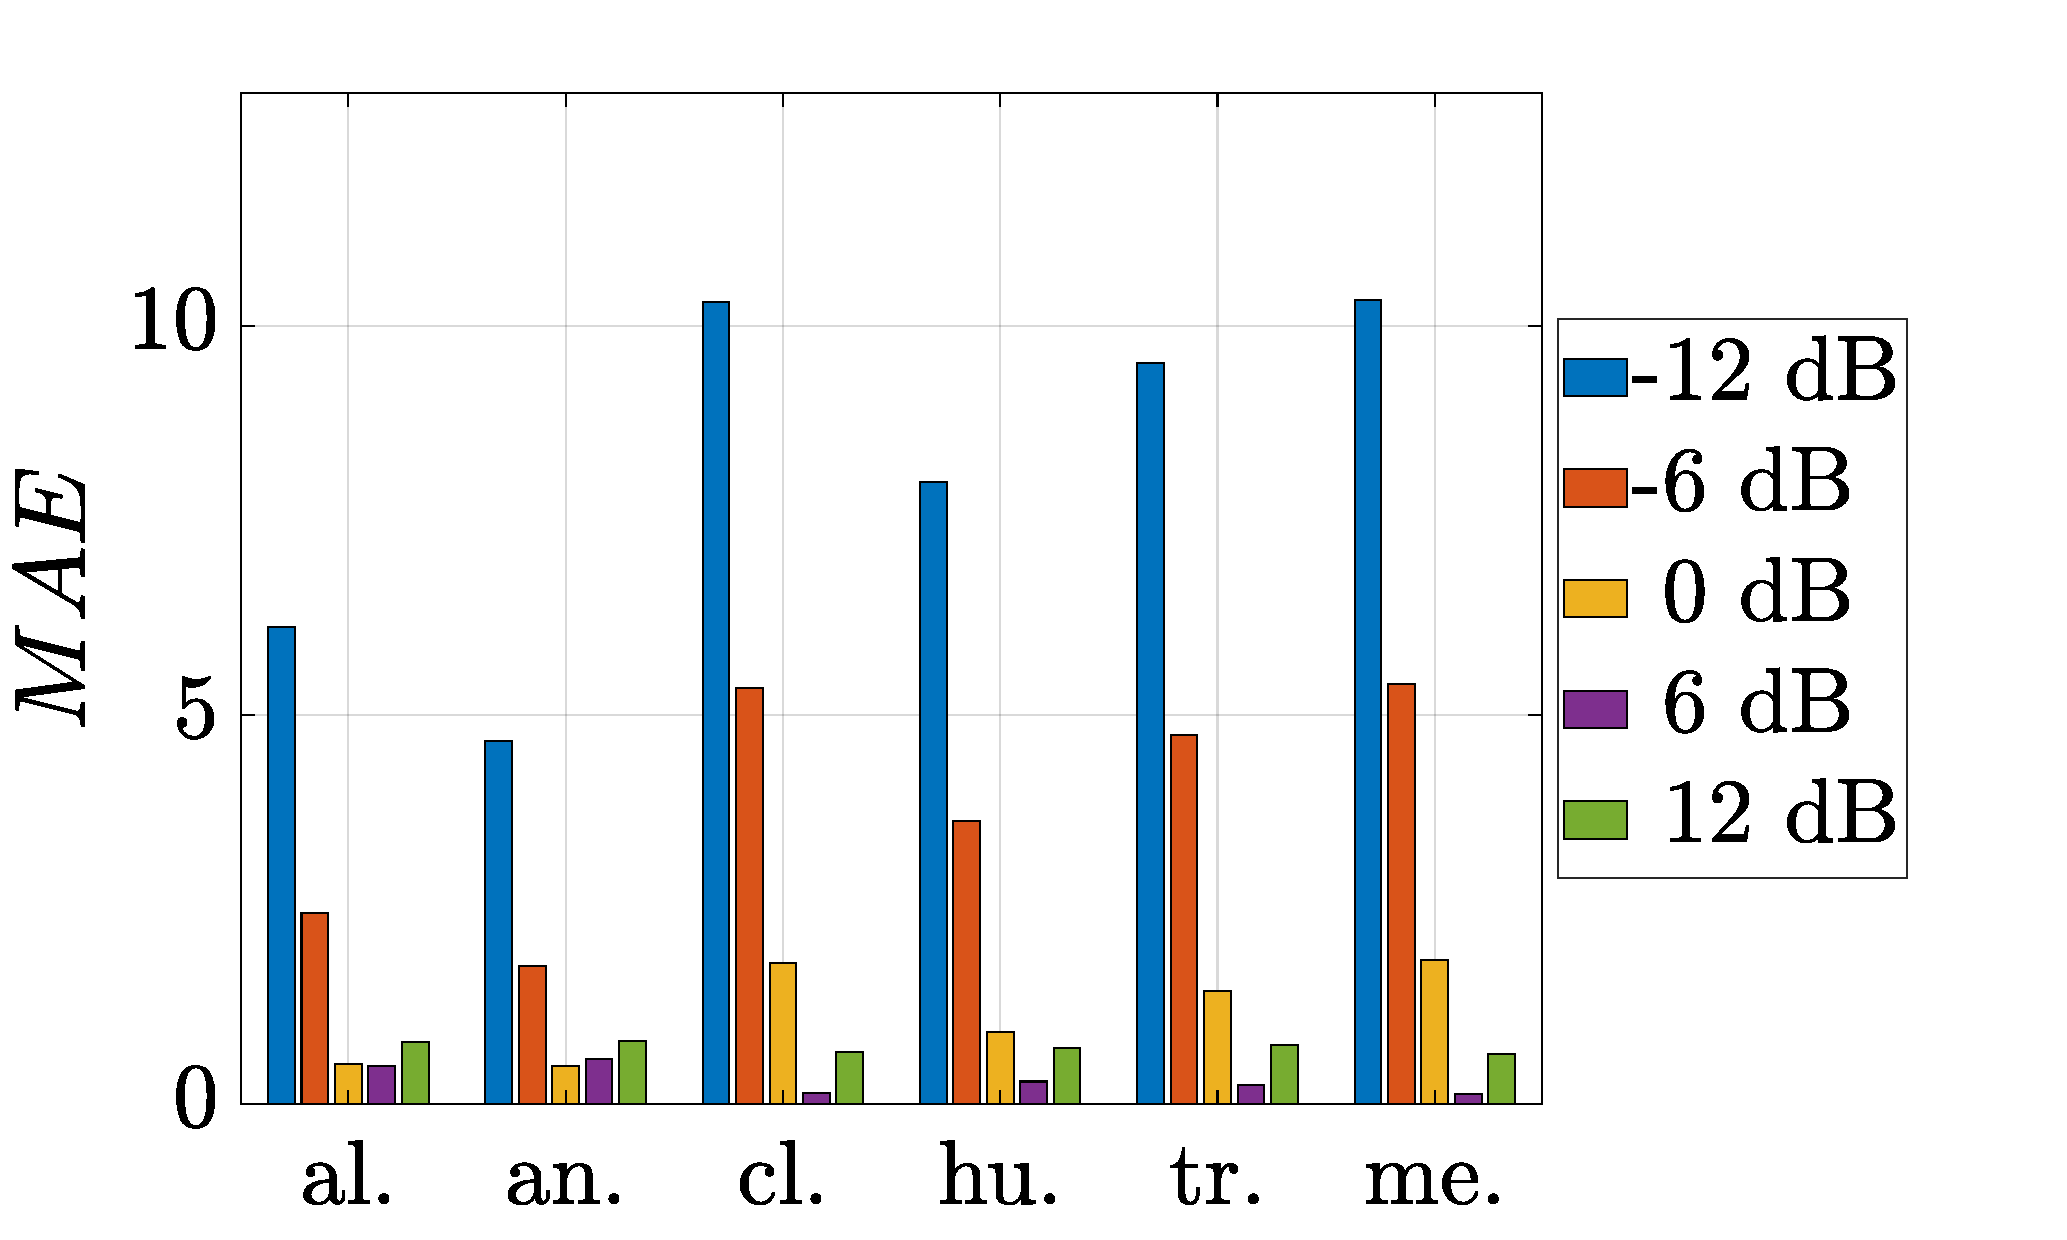
\includegraphics[width=0.60\linewidth]{./figures/resultats/ambiance_sup_bar.pdf}}%
\qquad
\subfigure[Erreurs $MAE$ pour la NMF SEM.]{%
\label{fig:TIR_class_semi}%
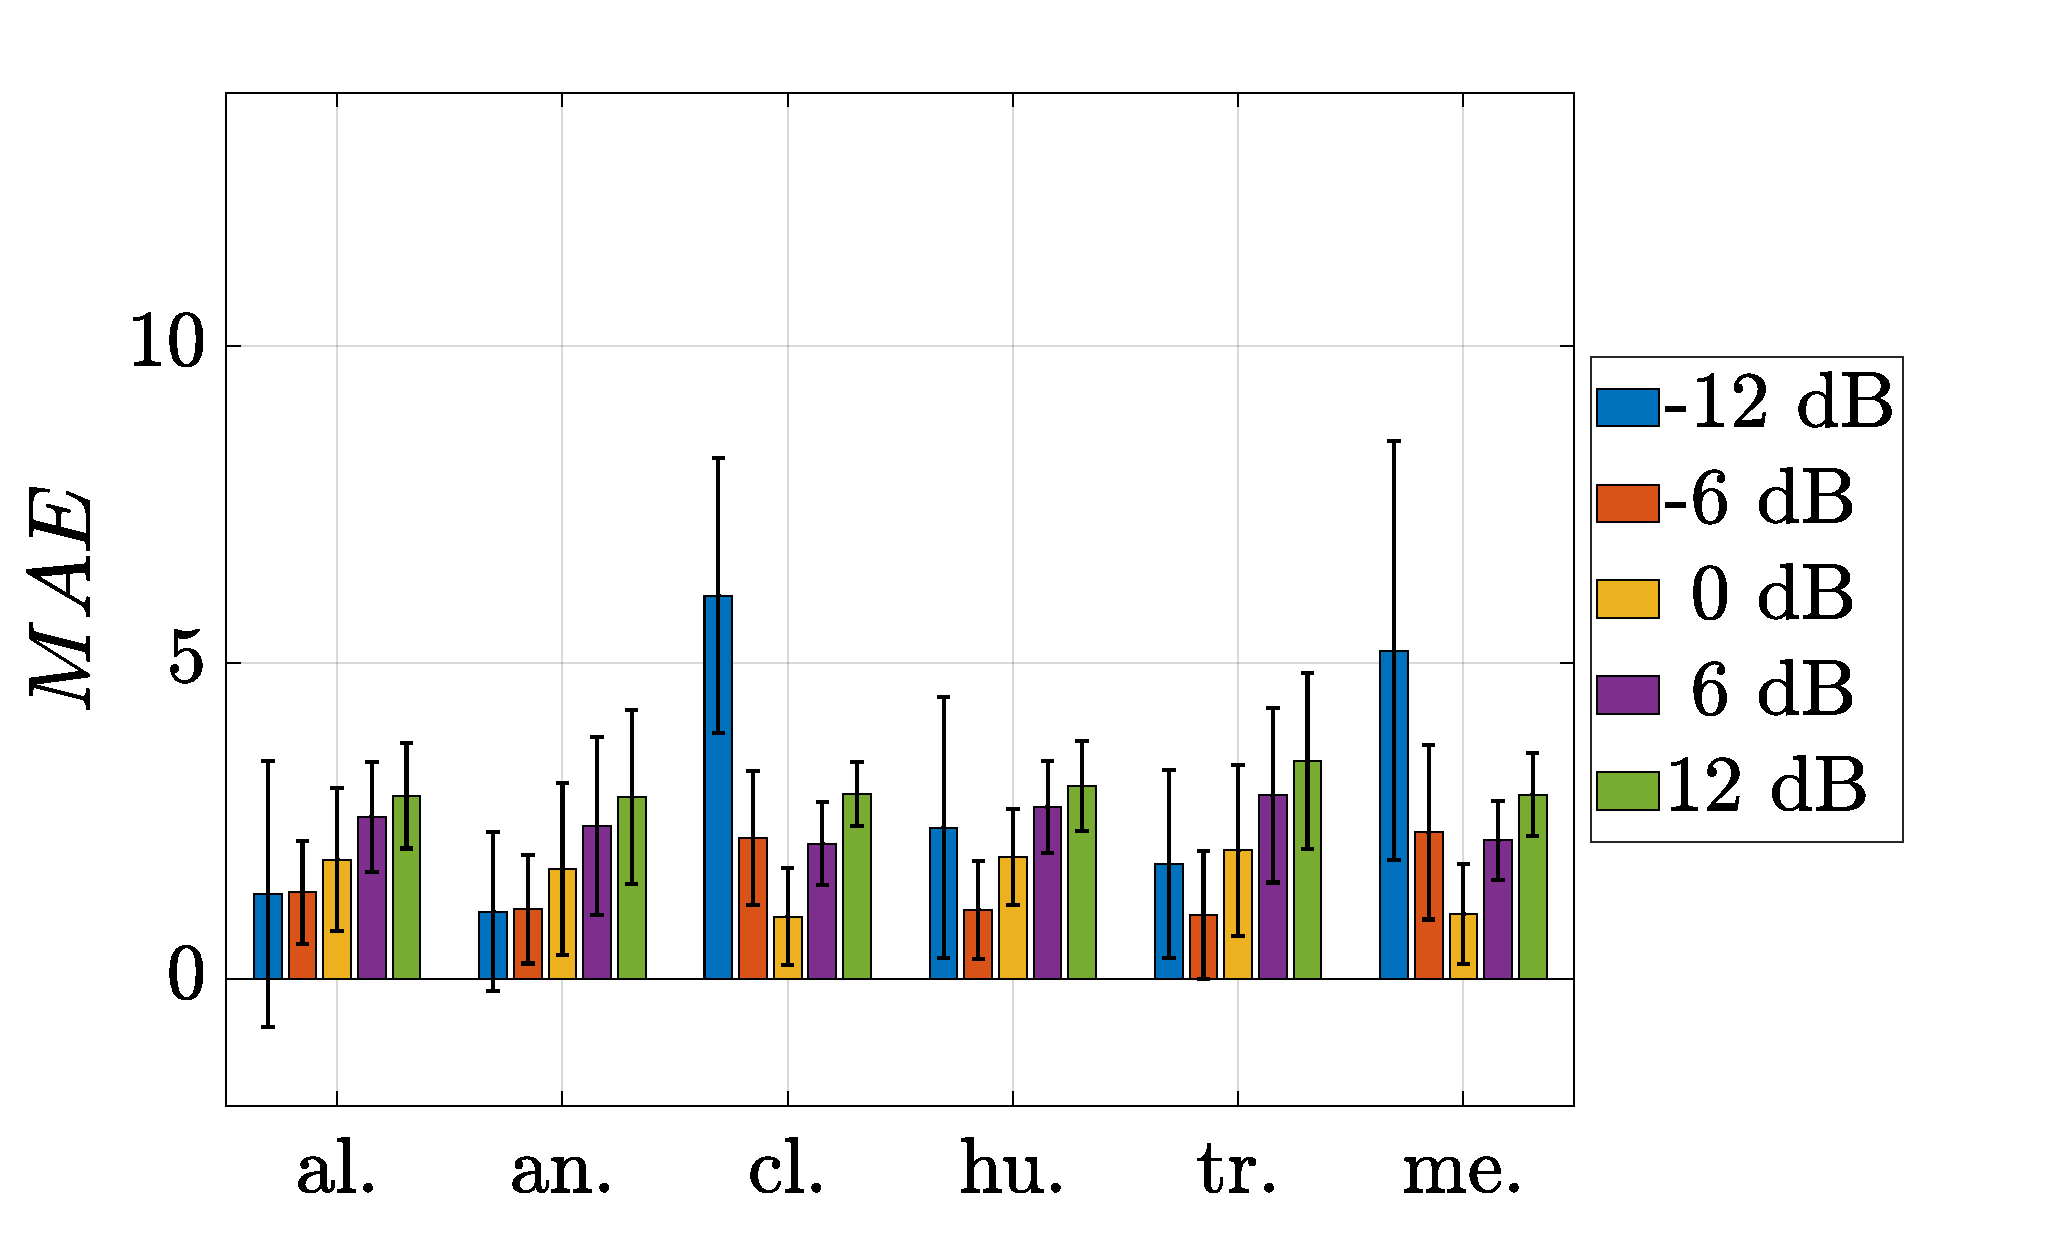
\includegraphics[width=0.60\linewidth]{./figures/resultats/ambiance_sem_bar.pdf}}%
\qquad
\subfigure[Erreurs $MAE$ pour la NMF IS.]{%
\label{fig:TIR_class_IS}%
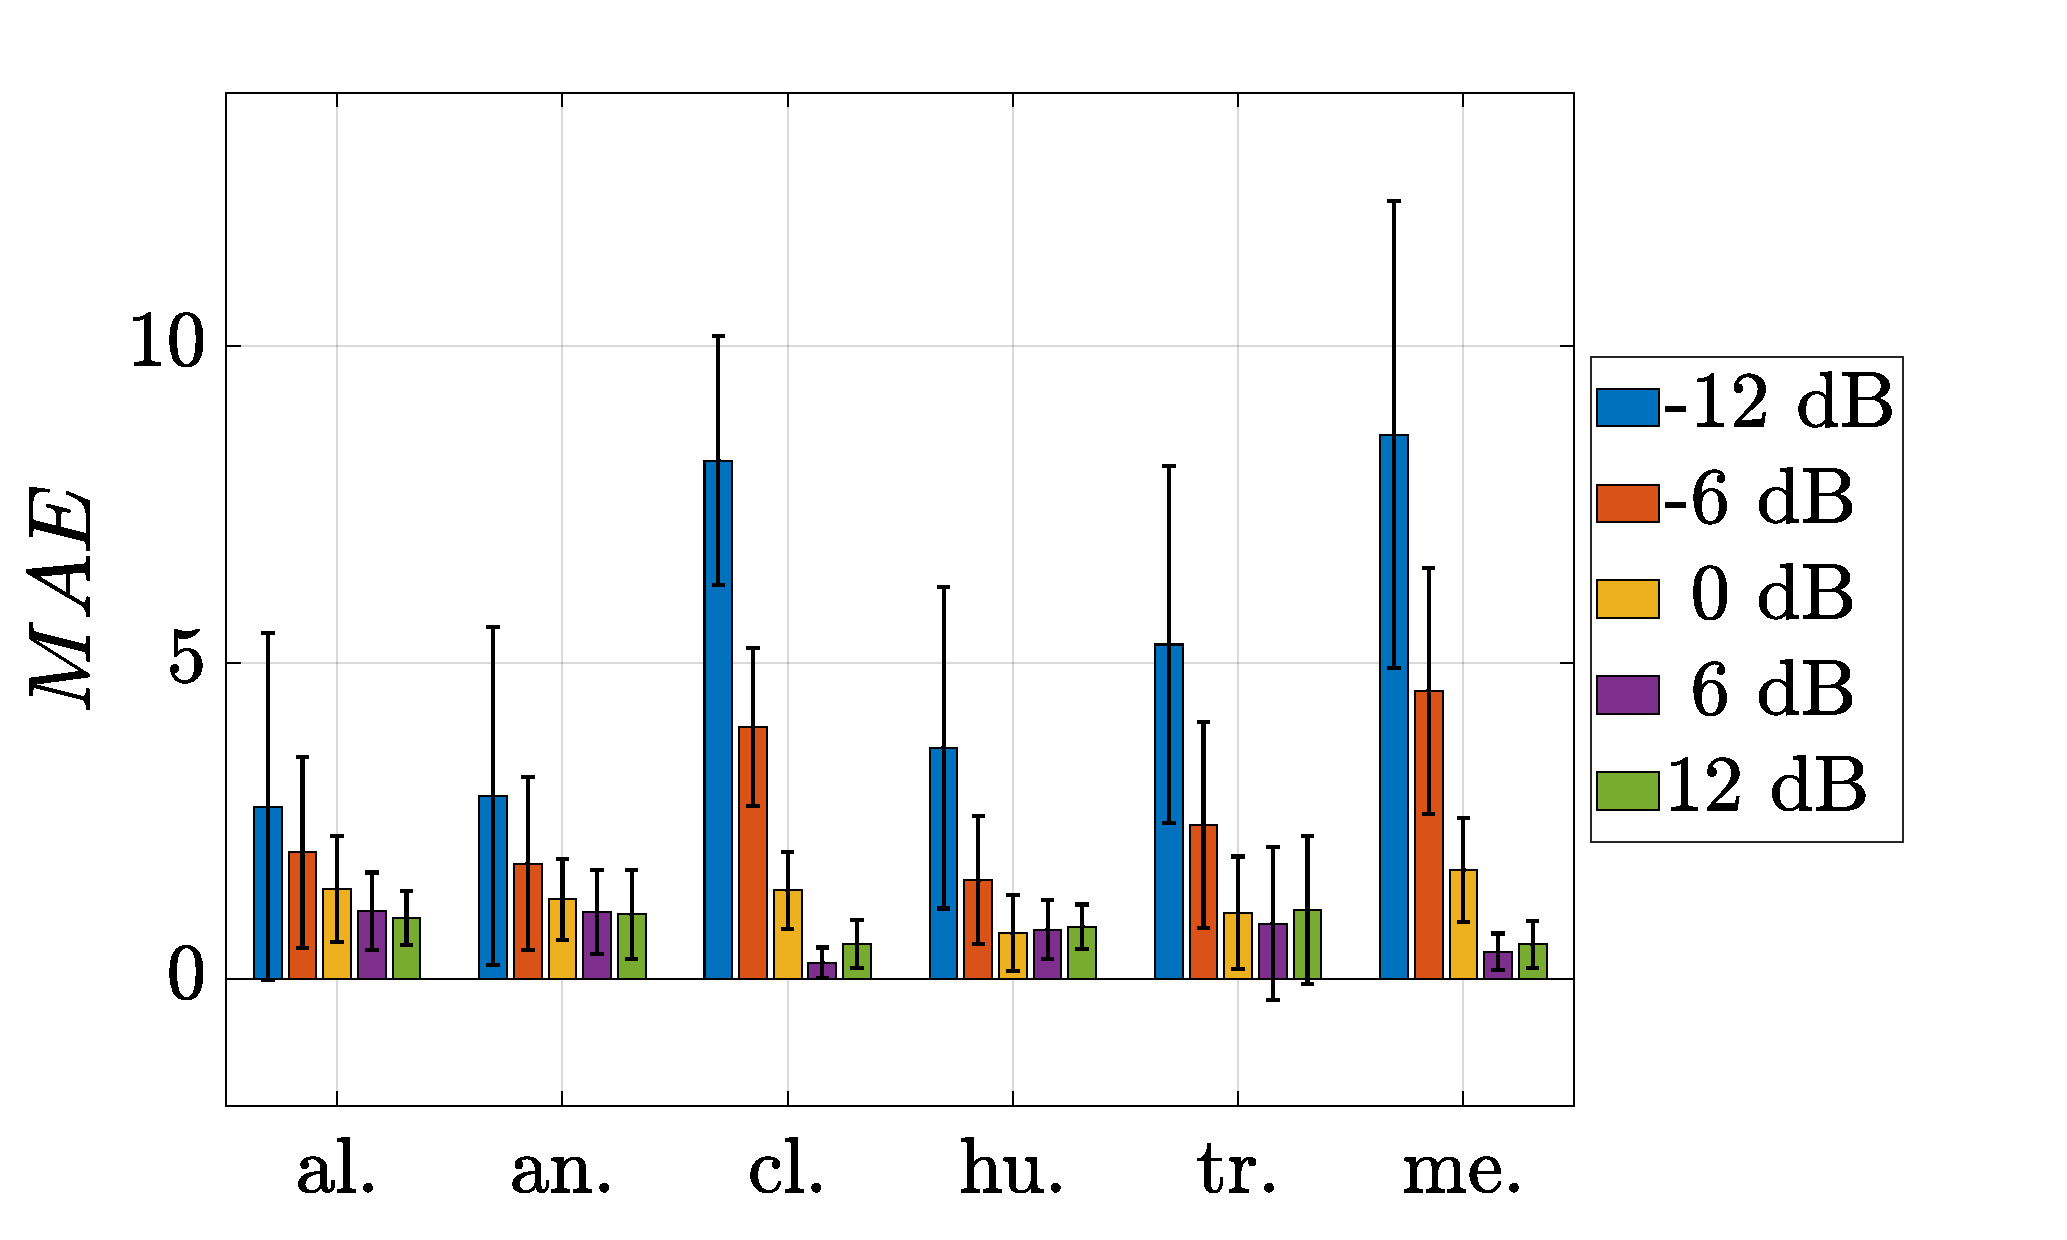
\includegraphics[width=0.60\linewidth]{./figures/resultats/ambiance_ti_bar.pdf}}%
\caption{Erreurs $MAE$ pour chaque classe pour la NMF SUP (\ref{fig:TIR_class_sup}), SEM (\ref{fig:TIR_class_semi}) et IS (\ref{fig:TIR_class_IS}).}
\label{fig:TIR_bar}
\end{figure}

De la même manière que pour l'estimateur filtre dans le Tableau \ref{tab:resuls_ambiance_filtre}, la méthode la plus efficace en moyenne sur l'ensemble du corpus n'est pas forcément la méthode la plus efficace pour chaque $TIR$. Ici, même si elle est pour quatre valeurs du $TIR$ inférieure à la baseline, la NMF IS n'est jamais la méthode qui propose l'erreur la plus faible. Pour $TIR \in \lbrace -12, -6 \rbrace$ dB, la NMF SEM est la plus performante, alors que pour $TIR\in \lbrace 6, 12 \rbrace$ dB, la NMF SUP supplante les deux autres méthodes.
Le cas où $TIR$ = 0 dB est un cas unique où aucune NMF n'améliore les résultats de la baseline. Pour $TIR$ = 12 dB c'est finalement le filtre $f_c$ = 20 kHz (c'est-à-dire l'absence de filtrage), qui se trouve être la méthode la plus performante. Lorsque, le niveau du trafic est très important, sa meilleur estimation est le niveau global de la mixture. Il vaut donc mieux ne rien faire sur le signal de mixture que d'appliquer la NMF. Ce résultats peut paraître décevant mais le problème est que, sur un problème concret, on ne connait pas le niveau à priori du trafic. 
Toutefois, la NMF IS est la seule méthode à être systématiquement inférieure à la baseline (hormis à $TIR = 0$ dB) et même si elle n'est pas systématiquement la plus performante, elle est celle qui s'adapte le mieux aux différentes valeurs du $TIR$. Les raisons du comportement des 3 NMF seront étudiés dans la partie suivante. \\


\subsection{Erreurs $MAE$ pour chaque ambiance et $TIR$}
Après avoir observé l'erreur globale $MAE_g$, pour déterminer les combinaisons de modalités qui proposent les erreurs moyennes les plus faibles, et l'erreur moyenne selon chaque $TIR$, l'erreur $MAE$ est maintenant observée. Cette erreur est calculée à partir des niveaux sonores exacts, $L_{eq,tr.}$, et estimés, $\tilde{L}_{eq,tr.}$ sur l'ensemble des 25 scènes pour chaque valeur de $TIR$ et sous-corpus.

Dans les Figures \ref{fig:TIR_bar}, les erreurs $MAE$ des 3 méthodes NMF optimales pour chaque $TIR$ et chaque ambiance sont exposées. La Figure \ref{fig:TIR_class_sup} permet de visualiser les performances très variables de la NMF SUP. Dans le cas où $TIR$ = $\lbrace -12, -6 \rbrace$ dB, et cela pour les 6 sous-corpus, la NMF SUP obtient de fortes erreurs $MAE$. Les plus fortes erreurs sont obtenues pour les sous corpus \textit{climat}, \textit{humains}, \textit{transport} et \textit{mécanique} car on y trouve les classes de son interférantes dont les allures spectrales sont les plus similaires à celles du trafic.
Même pour les sous-corpus \textit{alerte} et \textit{animaux}, la méthode échoue à obtenir des faibles erreurs. Ces performances sont toutefois contre-balancées par des erreurs beaucoup plus faibles dans les $TIR$ positifs, notamment à $TIR$ = 6 dB. La présence exclusive d'élément \textit{trafic} dans le dictionnaire sur des scènes où cette classe de son est prépondérante rend la NMF plus performante quel que soit le sous-corpus.

On illustre le comportement de la NMF SUP dans le cas d'une scène de l'ambiance \textit{alerte} pour $TIR$ = -12 dB et $TIR$ = 12 dB dans la Figure \ref{fig:Lp_alert} où les évolutions du $L_{eq,1s}$ des signaux \textit{trafic} exact, \textit{trafic} estimé par la NMF SUP optimale et du signal \textit{interférant} sont tracées. Dans le cas où le $TIR$ est négatif, lorsque le signal \textit{interférant} est émergent, on observe que le signal \textit{trafic} estimé inclut ce signal. N'étant composé que d'éléments \textit{trafic} dans le dictionnaire c'est donc que les bases \textit{trafic} de $\mathbf{W}$ sont activées pour modéliser un signal qui ne l'est pourtant pas. Ce comportement disparait toutefois pour $TIR$ = 12 dB où le signal \textit{trafic} est correctement modélisé sans être impacté par la classe de son interférante.

\begin{figure}[h!]%
\centering
\subfigure[Comparaison du niveau sonore  pour $TIR$ = -12 dB pour la scène 25 du sous-corpus \textit{alerte}.]{%
\label{fig:Lp_alert_-12}%
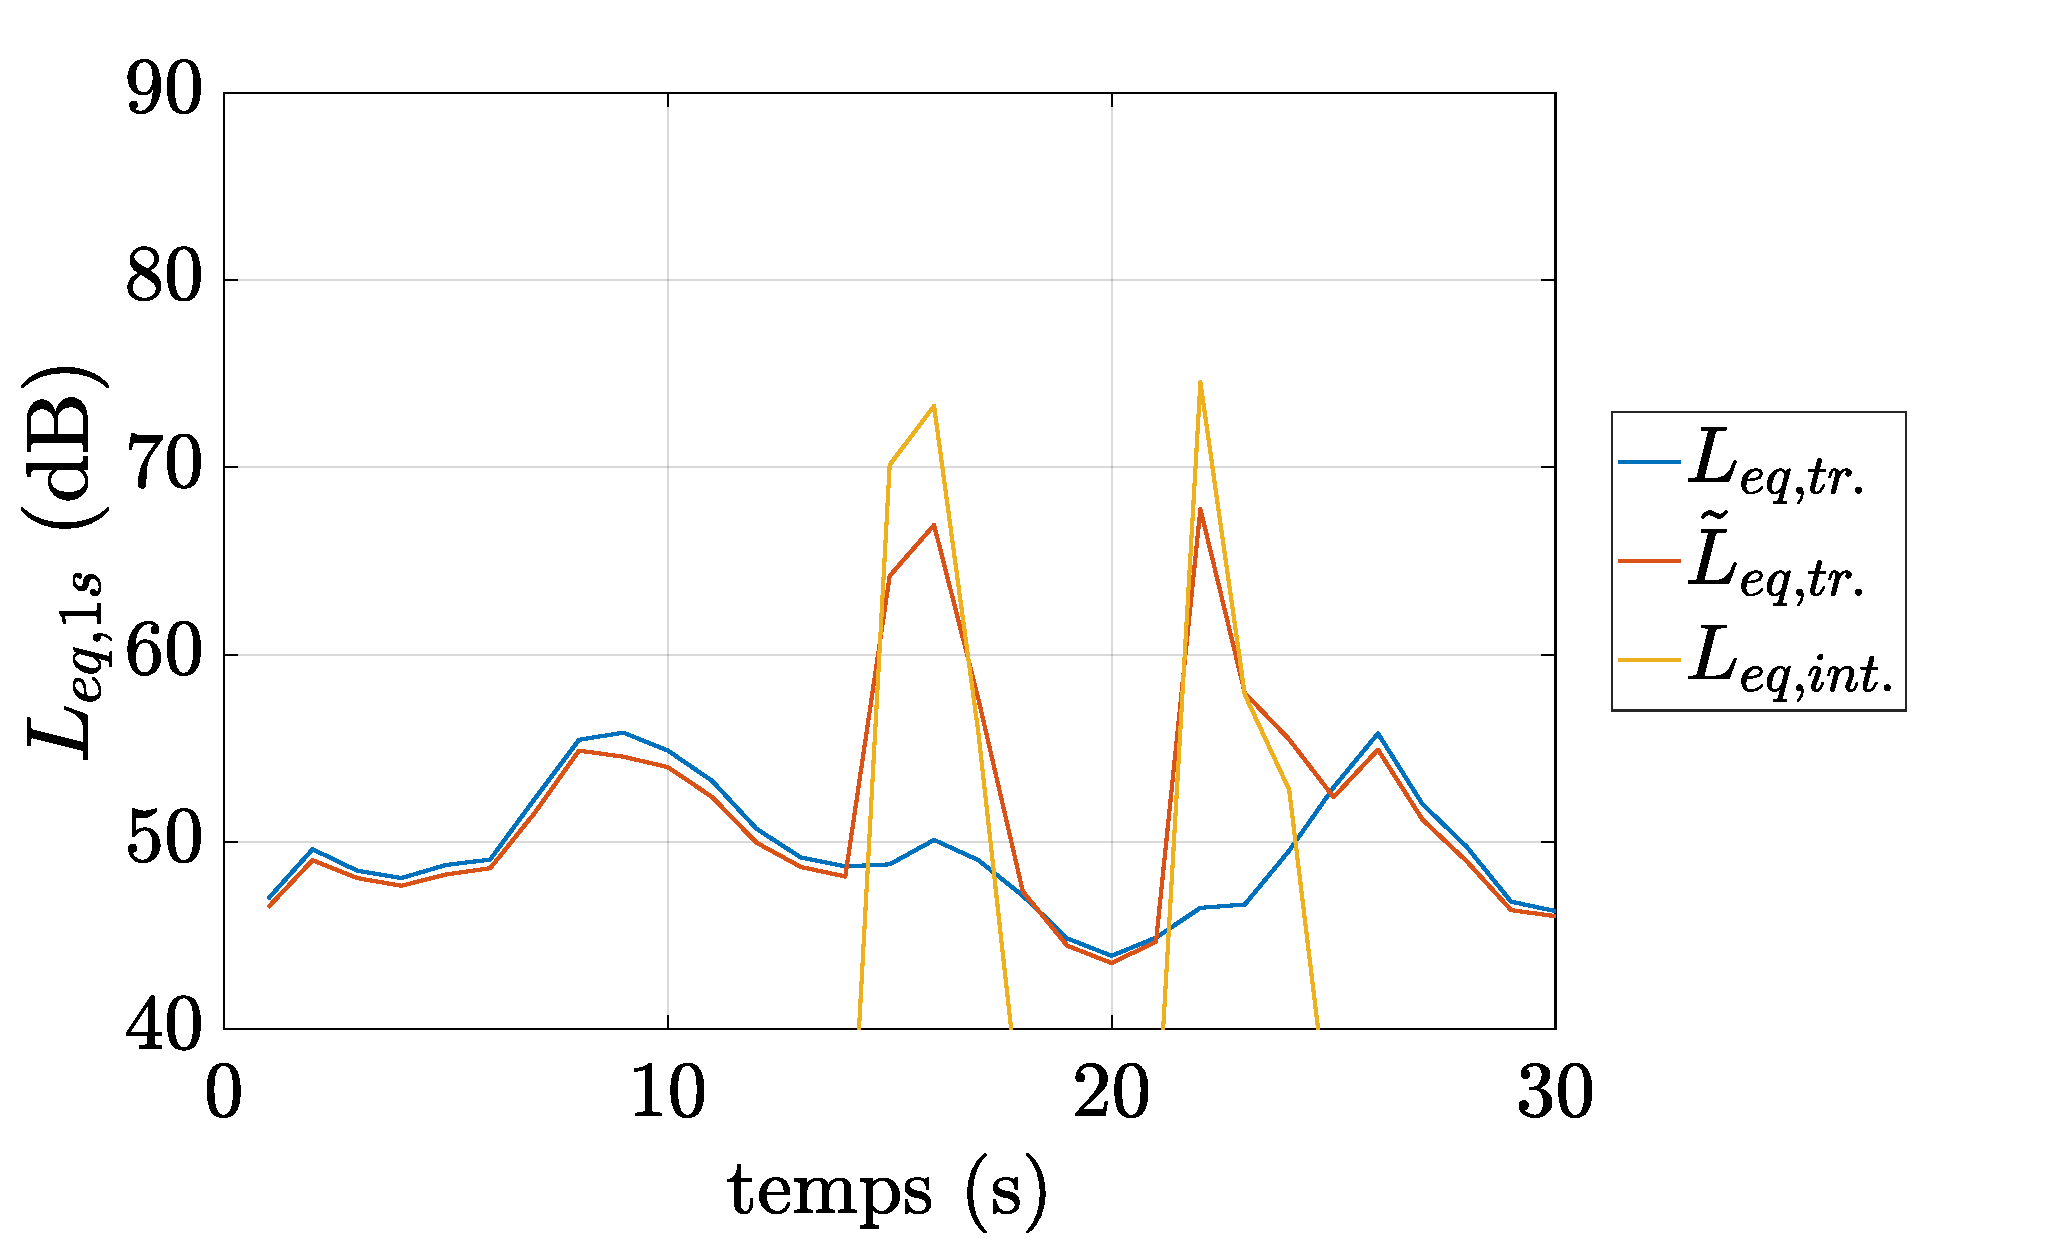
\includegraphics[width=0.450\linewidth]{./figures/resultats/Lp_alert_SUP_-12.pdf}}%
\qquad
\subfigure[Comparaison du niveau sonore  pour $TIR$ = 12 dB pour la scène 25 du sous-corpus \textit{alerte}.]{%
\label{fig:Lp_alert_12}%
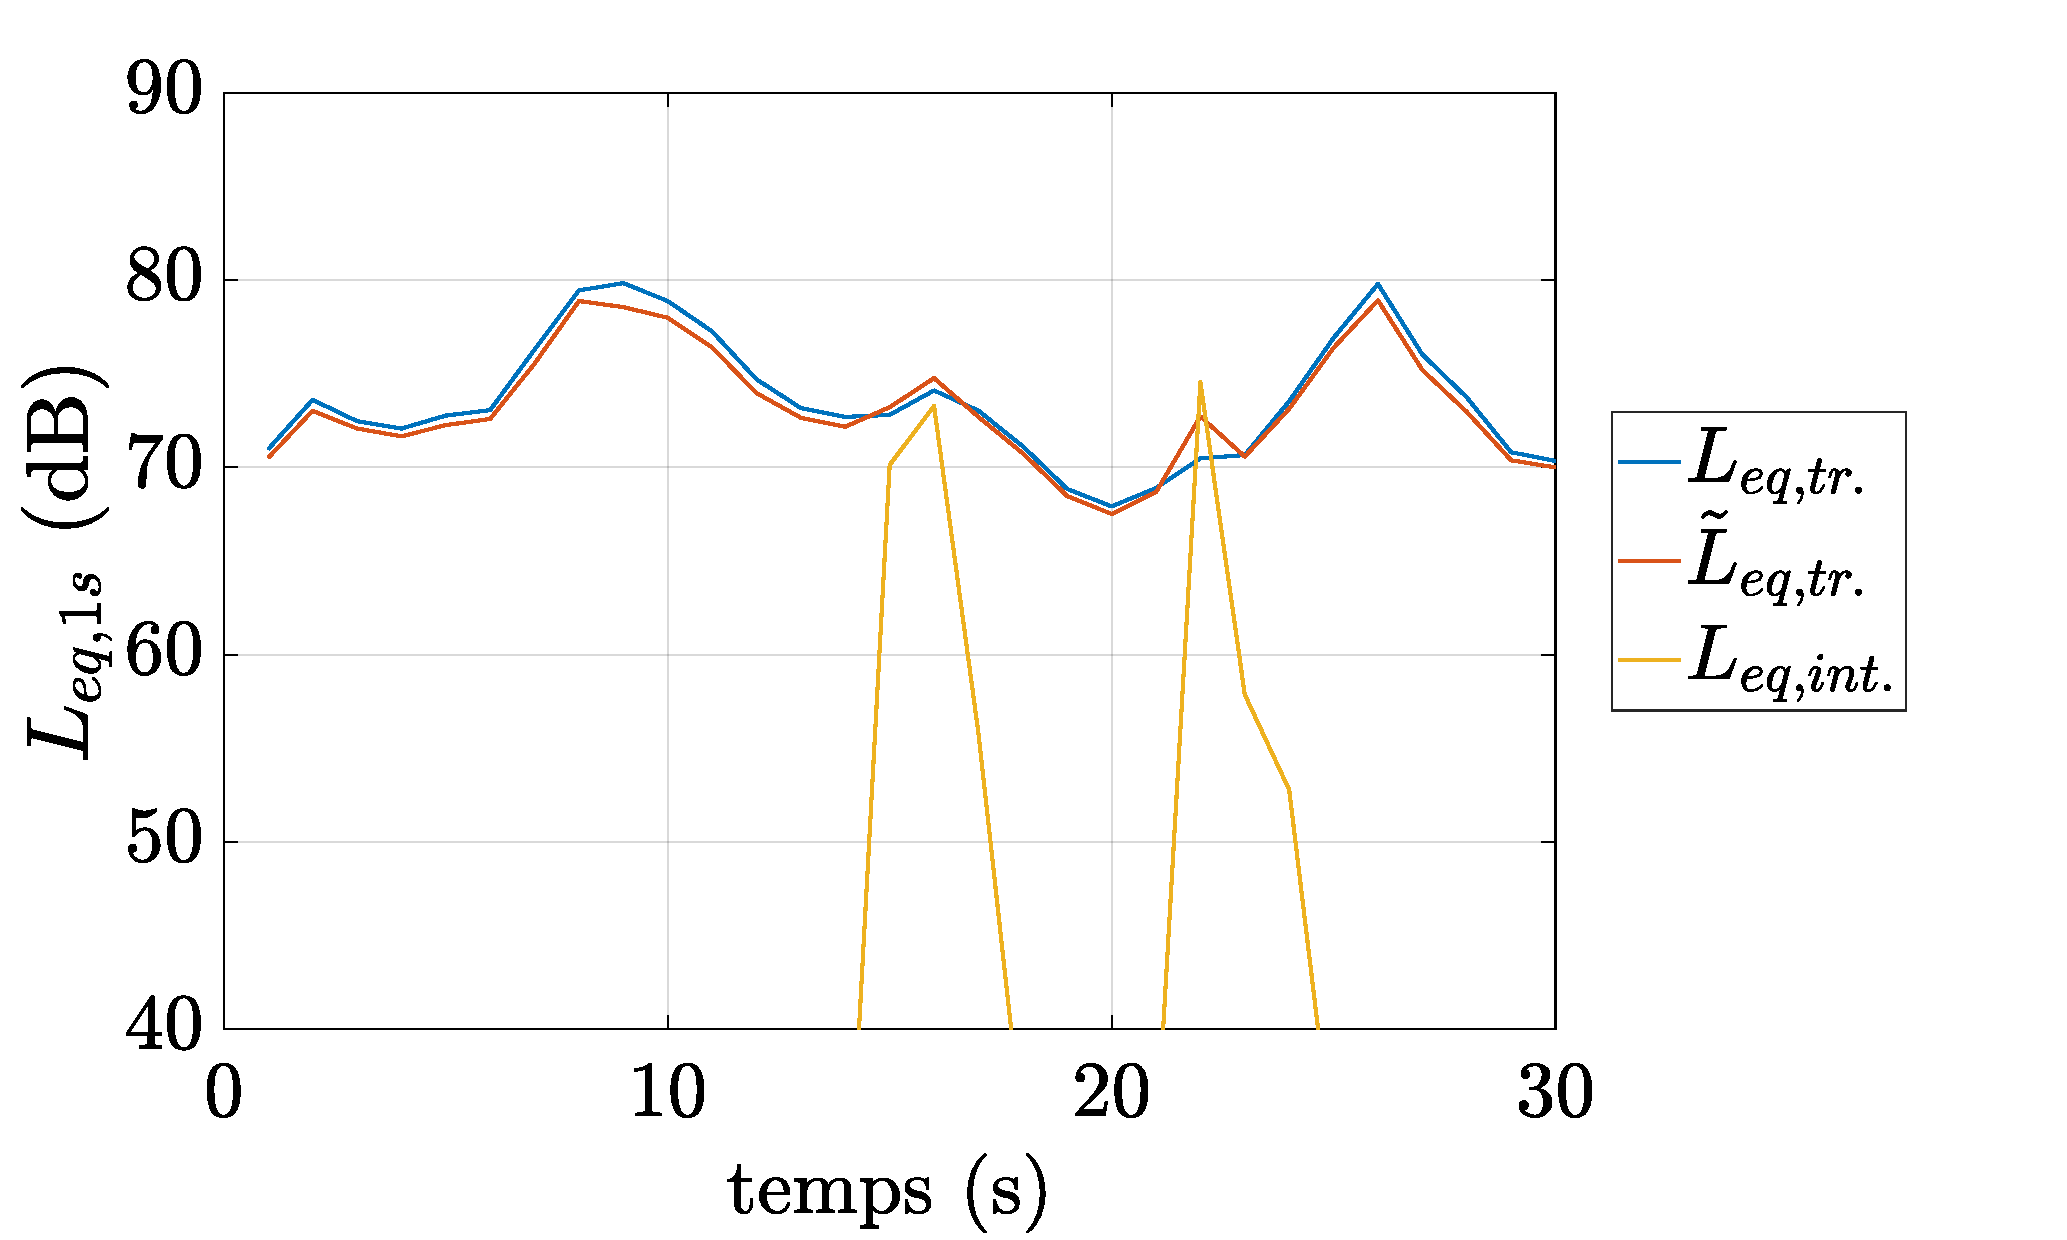
\includegraphics[width=0.450\linewidth]{./figures/resultats/Lp_alert_SUP_12.pdf}}%
\caption{Comparaisons des niveaux sonores équivalents des classes \textit{trafic} et \textit{interférante} pour 2 valeurs du $TIR$ (-12 dB et 12 dB) pour la scène 25 du sous-corpus \textit{alerte}.}
\label{fig:Lp_alert}
\end{figure}

\begin{figure}[h!]%
\centering
\subfigure[Comparaison pour $TIR$ = -12 dB pour la scène 2 du sous-corpus \textit{alerte}.]{%
\label{fig:Y_alert_-12}%
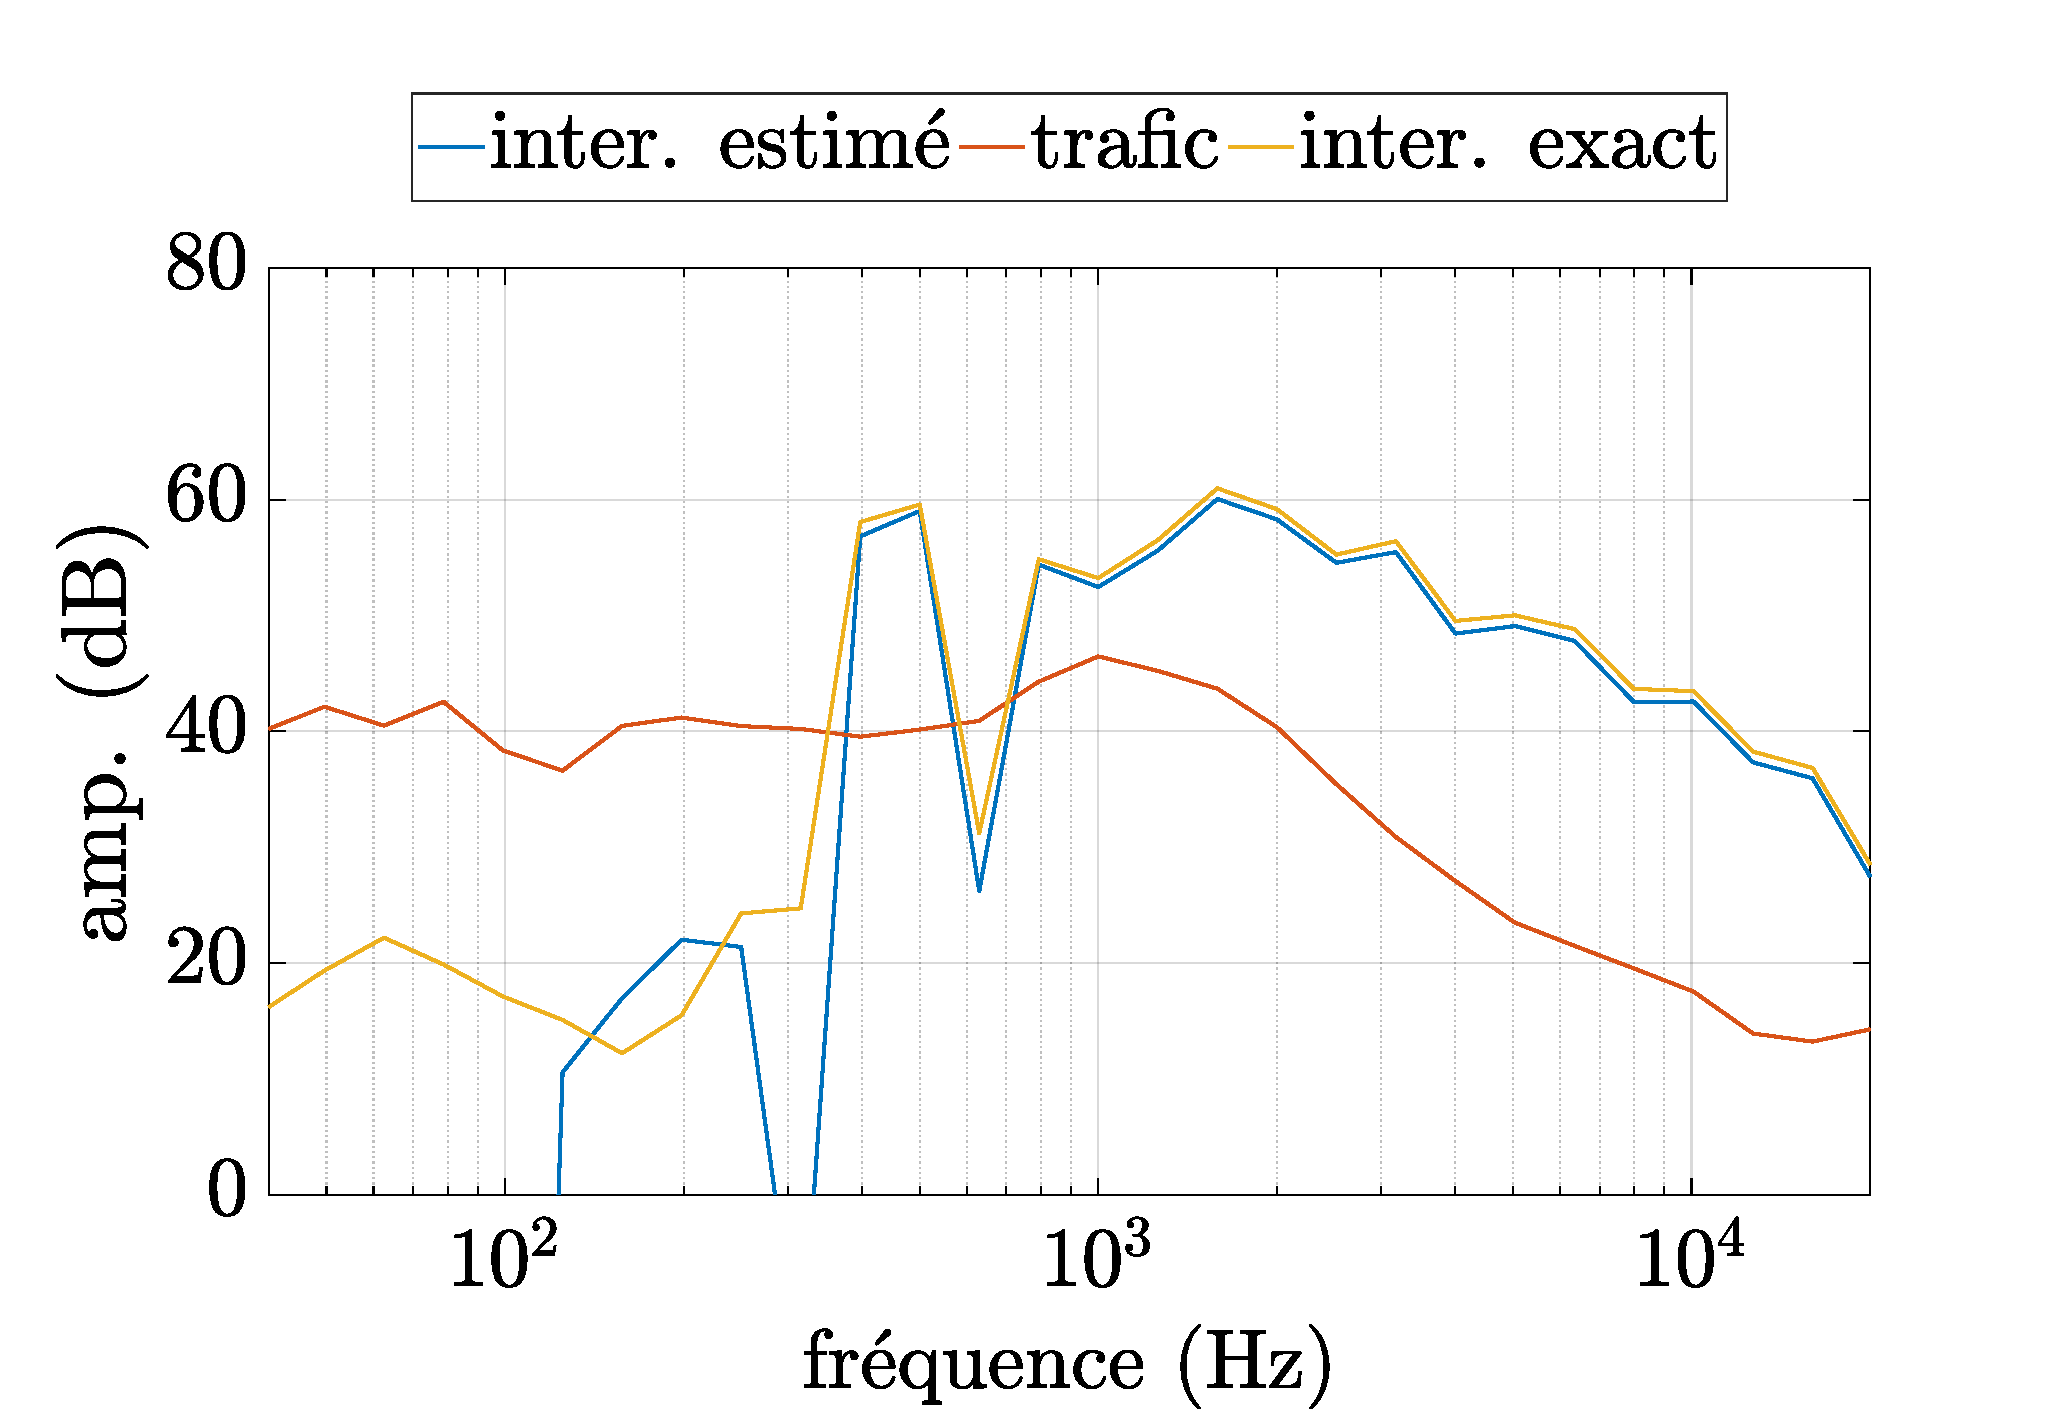
\includegraphics[width=0.450\linewidth]{./figures/resultats/alert02_tir-12_Y.pdf}}%
\qquad
\subfigure[Comparaison pour $TIR$ = 12 dB pour la scène 2 du sous-corpus \textit{alerte}.]{%
\label{fig:Y_alert_12}%
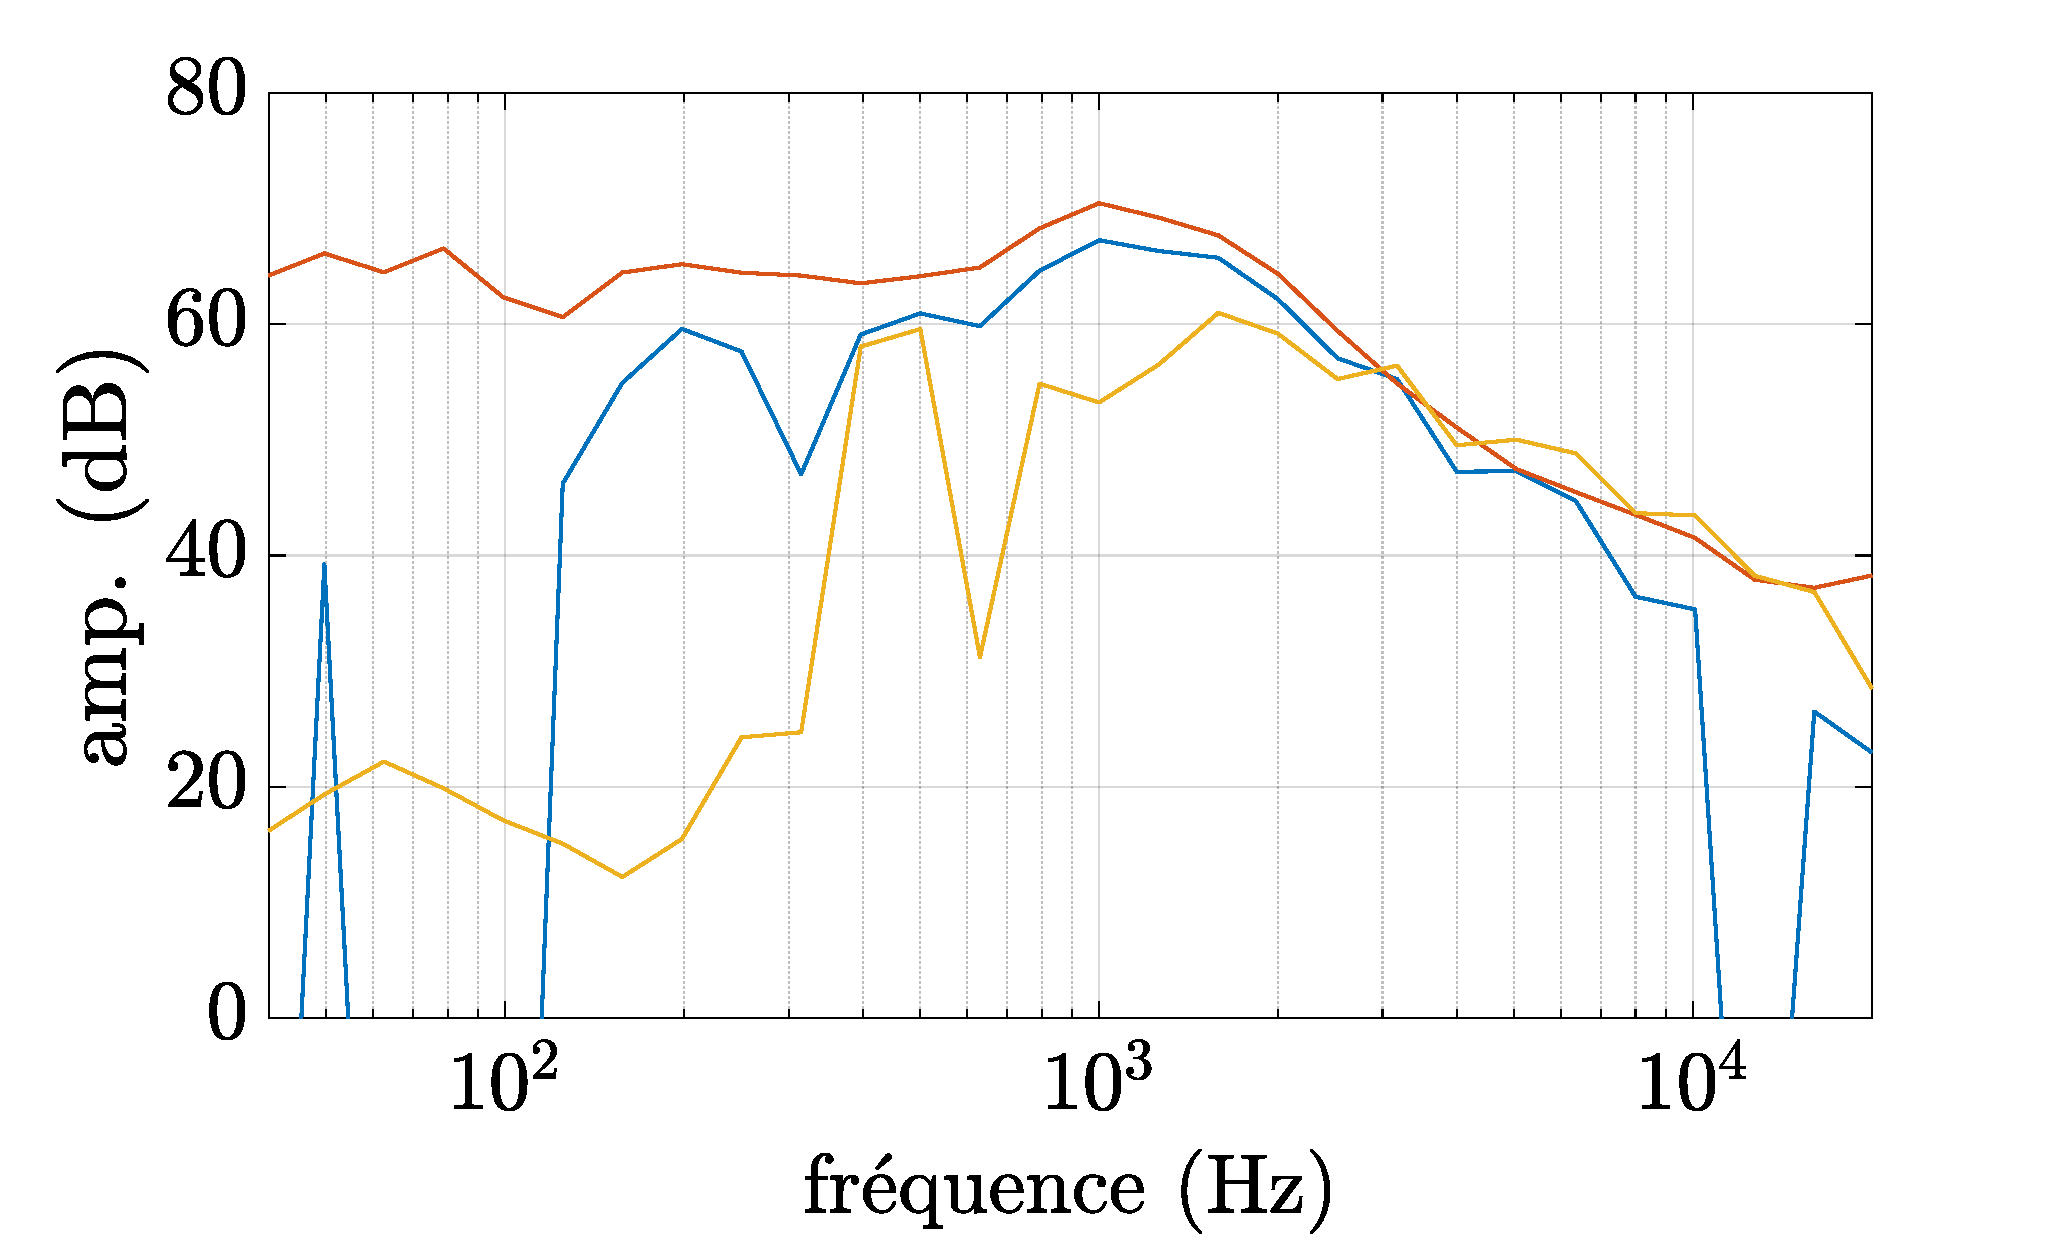
\includegraphics[width=0.450\linewidth]{./figures/resultats/alert02_tir12_Y.pdf}}%
\qquad
\subfigure[Comparaison pour $TIR$ = -12 dB pour la scène 3 du sous-corpus \textit{climat}.]{%
\label{fig:Y_climat_-12}%
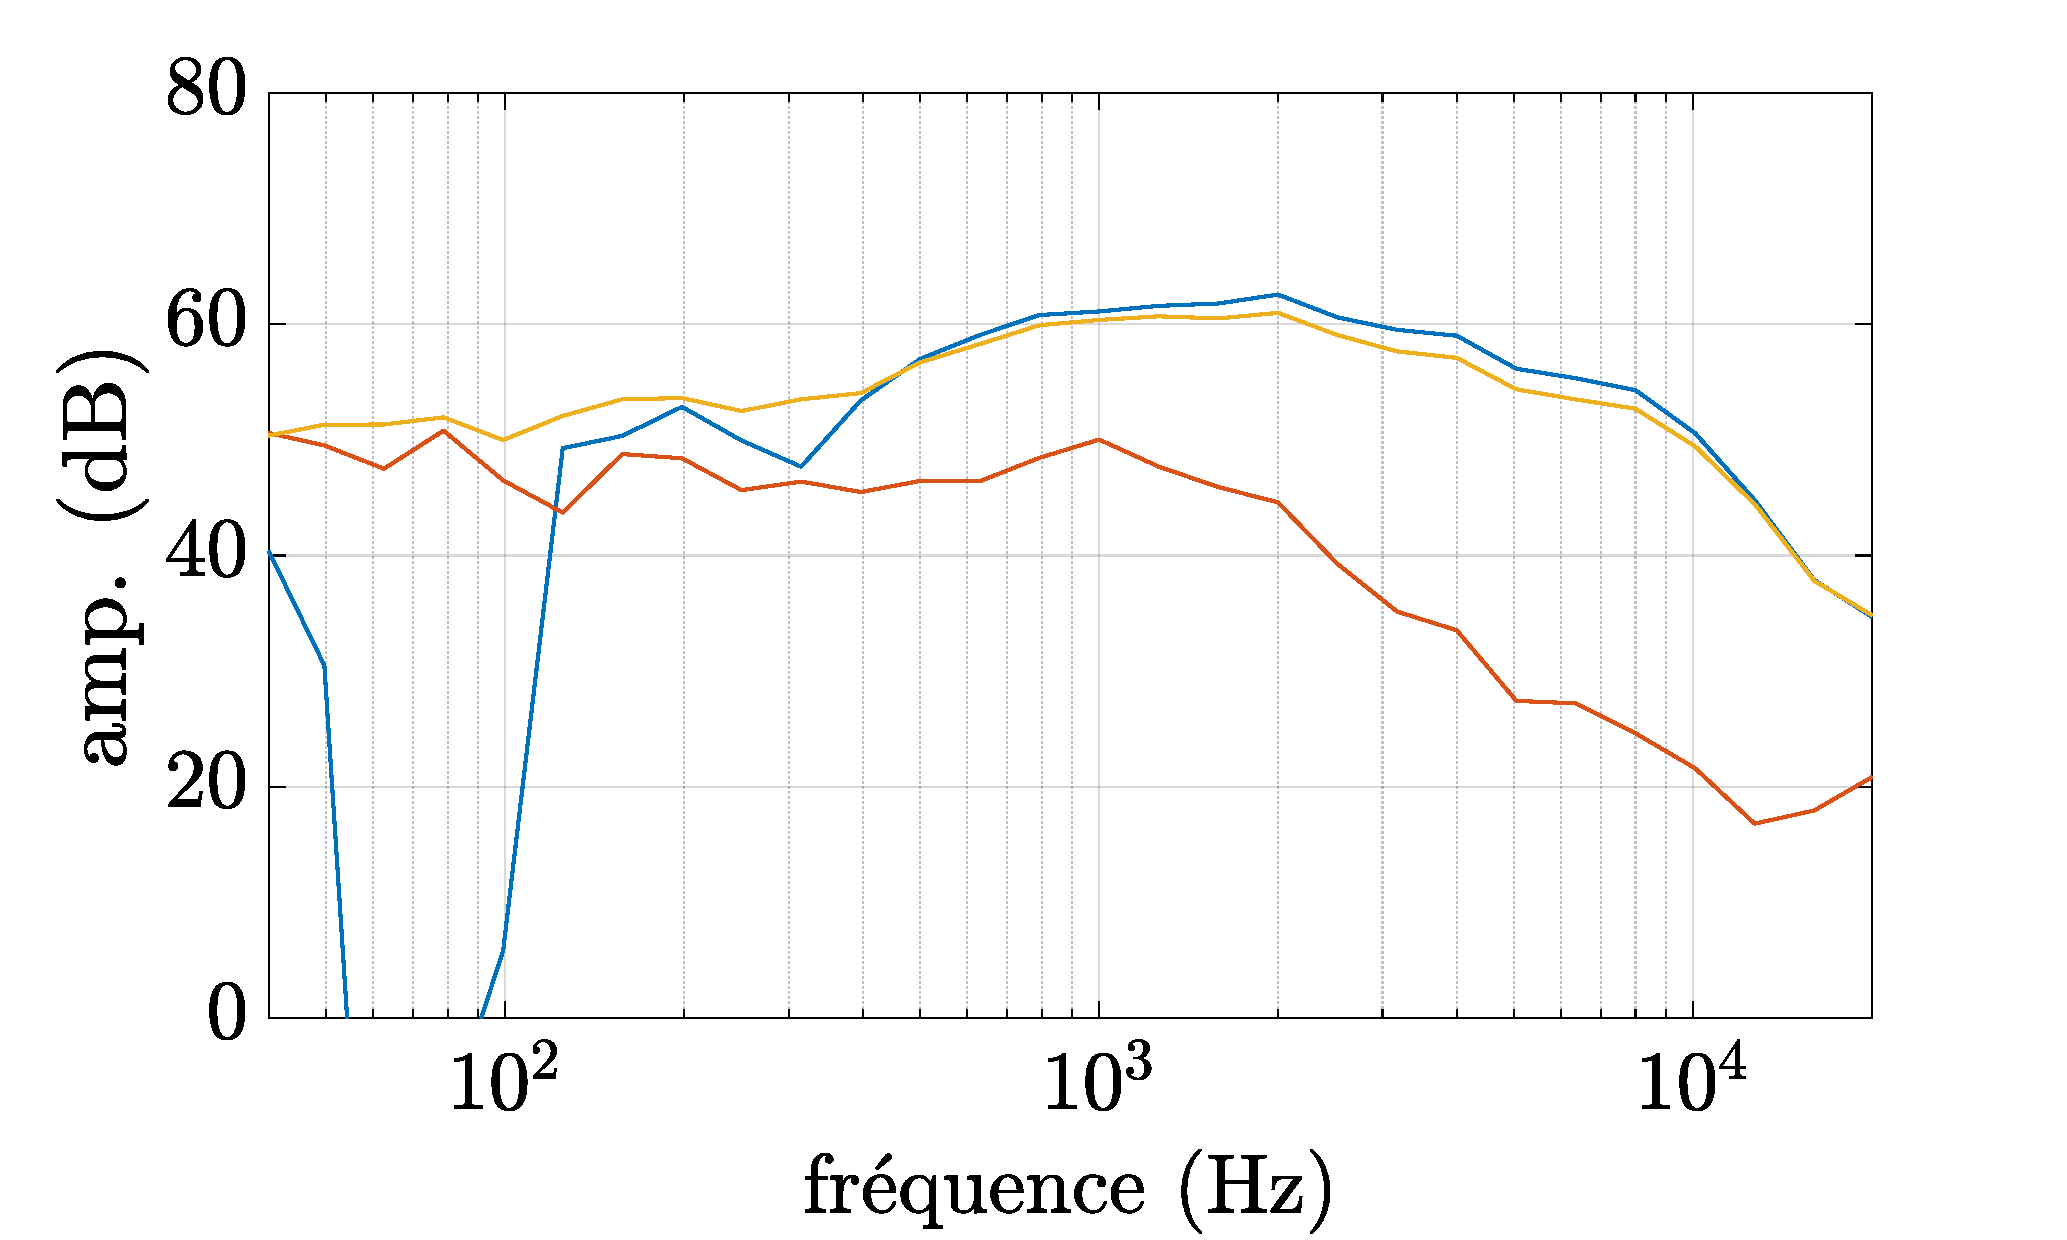
\includegraphics[width=0.450\linewidth]{./figures/resultats/climat03_tir-12_Y.pdf}}%
\qquad
\subfigure[Comparaison pour $TIR$ = 12 dB pour la scène 3 du sous-corpus \textit{climat}.]{%
\label{fig:Y_climat_12}%
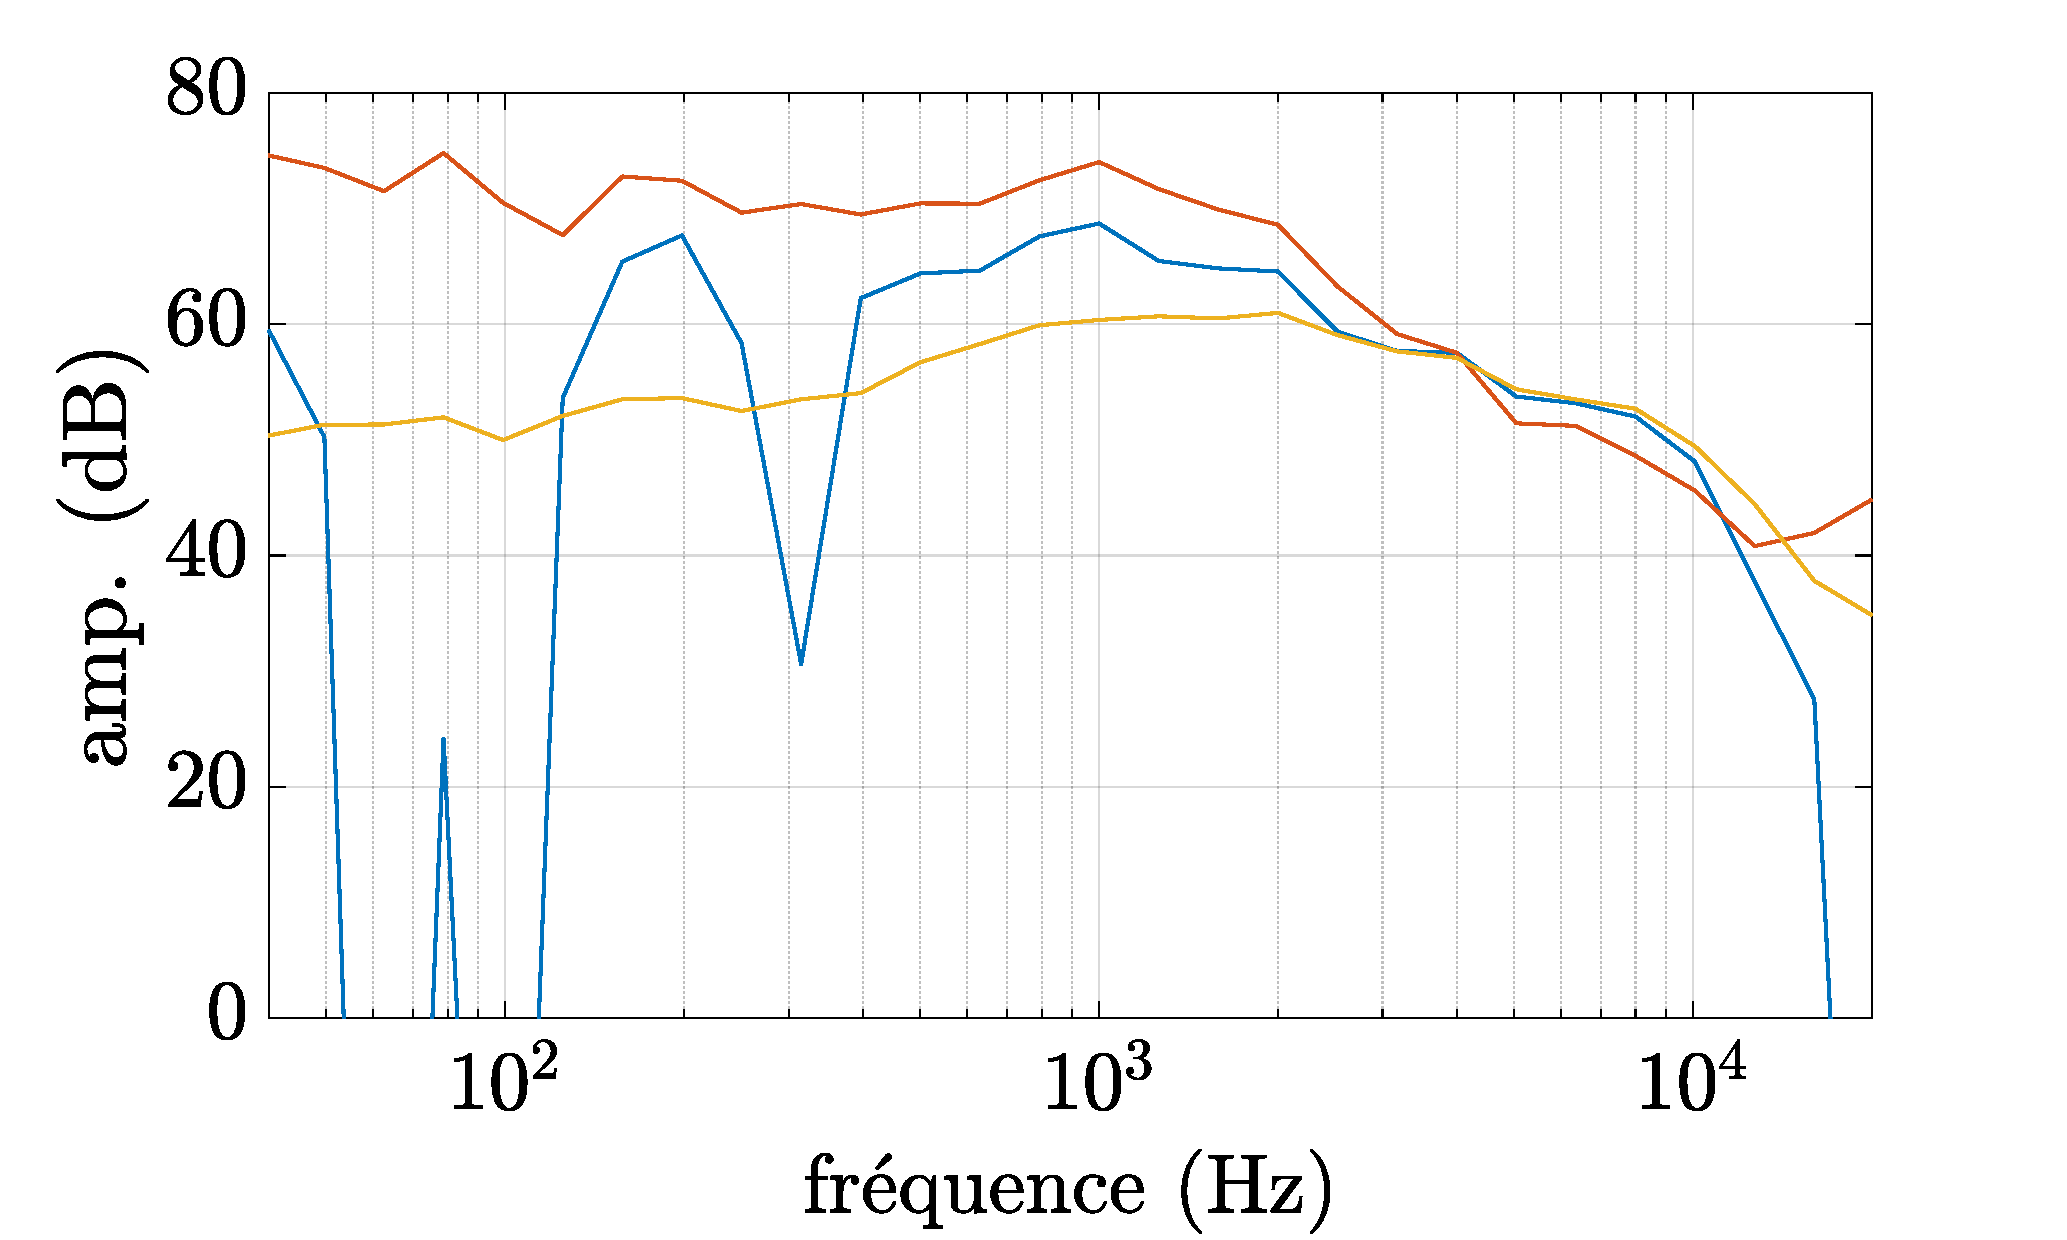
\includegraphics[width=0.450\linewidth]{./figures/resultats/climat03_tir12_Y.pdf}}%
\caption{Comparaisons des spectres des classes \textit{trafic} et \textit{interférante} avec la somme des 2 éléments de $\mathbf{W_r}$ pour 2 valeurs du $TIR$ (-12 dB et 12 dB) pour 2 sous-corpus (\textit{alerte} et \textit{climat)}.}
\label{fig:Y_ambiance}
\end{figure}

La NMF SEM (Figure \ref{fig:TIR_class_semi}) présente un comportement différent de la NMF SUP : les erreurs sont plus faibles lorsque les valeurs du $TIR$ sont négatives, hormis pour les sous-corpus \textit{climat}  et \textit{mécanique}. L'ajout de $\mathbf{W_r}$ dans le dictionnaire est donc déterminant puisque c'est cet élément qui différencie les deux méthodes. Cependant, lorsque le $TIR$ devient positif et le trafic dominant, l'erreur augmente systématiquement.
On compare dans les Figures \ref{fig:Y_ambiance} la somme des deux éléments de $\mathbf{W_r}$ obtenue pour une scène \textit{alerte} et \textit{climat} avec les spectres des signaux trafic et interférant à $TIR \in \lbrace -12, 12 \rbrace$ dB. Dans les cas où $TIR$ = -12 dB, la somme des éléments libres $\mathbf{W_r}$ correspond bien au spectre de la classe \textit{interférante} et modélise donc bien cette classe, laissant la partie \textit{trafic} au dictionnaire $\mathbf{W_s}$. À l'opposée, pour $TIR$ = 12 dB, l'allure de $\mathbf{W_r}$ diverge de celle de la classe \textit{interférante}. Certaines parties des spectres participent alors à la modélisation de la composante \textit{trafic}, ce qui réduit la justesse de son estimation du niveau sonore. Les degrés de liberté de la NMF SEM sont donc un avantage lorsque le trafic est peu présent car ils permettent bien d'intégrer la classe de son \textit{interférante}. Mais cette liberté joue en sa défaveur lorsque le trafic devient la classe de son prédominante et où ses composantes sont incluses dans $\mathbf{W_r}$.\\

Enfin, la NMF IS présente une allure similaire à celle de la NMF SUP (erreurs plus fortes pour les $TIR$ négatifs que dans les $TIR$ positifs), mais avec des erreurs moindres notamment pour les $TIR$ négatifs. Toutefois les erreurs pour les sous-corpus \textit{climat}, \textit{transport} et \textit{mécanique} restent élevées en raison de la proximité de leur spectre avec ceux du trafic. Pour $TIR \geq 0$, les erreurs restent faibles ($< 1,7$ dB). La valeur seuil de 0,41 est la valeur optimale permettant une erreur minimale sur l'intégralité du corpus, mais selon le sous-corpus ou le $TIR$ ce seuil est susceptible de varier.
Dans les Figures \ref{fig:TIR_mae}, l'évolution de l'erreur $MAE$ est tracée en fonction du seuil $t_h$ pour chaque sous-corpus et pour 3 valeurs de $TIR$.
\begin{itemize}
\item Pour $TIR$ = -12 dB, l'erreur $MAE$ minimale diffère selon les sous-corpus.
Pour les classes de son \textit{transport} et \textit{humains}, leur seuil optimal correspondant à l'erreur minimale est situé vers 0,50. Dans le cas du \textit{climat} et de \textit{mécanique}, ce seuil semble se situer au delà de la plage de variation testée.  Pour ces 4 sources, dont les erreurs à ces $TIR$ sont les plus fortes, leur spectre étant similaire à celui du \textit{trafic}, il y a intérêt à augmenter la valeur du seuil $t_h$ pour restreindre le nombre d'éléments dans $\mathbf{W}_{trafic}$. À l'inverse pour  les classes \textit{animaux} et \textit{alerte}, dont l'allure spectrale est différente de celle du trafic, le seuil optimal peut être diminué.
Ainsi, la valeur seuil optimale pour $TIR$ = -12 dB peut être relevée à $t_h = 0,49$, sur l'ensemble des sous-corpus pour une erreur $MAE_{-12}$ = 4,61 ($\pm$ 1,91) avec alors un nombre moyen d'éléments $K$ = 79 ($\pm$ 22).
\item Lorsque $TIR$ = 0 dB, le trafic devenant prédominant, le dictionnaire $\mathbf{W'}$ mis à jour contient plus d'éléments trafic. En diminuant le seuil $t_h$, plus d'éléments relatif à cette source sonore sont intégrés dans $\mathbf{W'}$.
Les classes de sons \textit{climat} et de \textit{mécanique} restent encore en marge avec un seuil optimal élevé situé entre 0,45 et 0,50.
\item Enfin, pour $TIR$ = 12 dB, pour un seuil optimal $t_h$ = 0,31, un plus grand nombre d'éléments du dictionnaire est considéré ($K_{moyen}$ = 142 ($\pm$ 22)), l'erreur $MAE_{+12}$ diminue alors à 0,20 ($\pm$ 0,08), soit même une erreur inférieure au filtre passe-bas à 20 kHz (correspondant à la mixture sonore complète).\\
\end{itemize}

\begin{figure}[h!]%
\centering
\subfigure[]{%
\label{fig:TIR_mae_tir-12}%
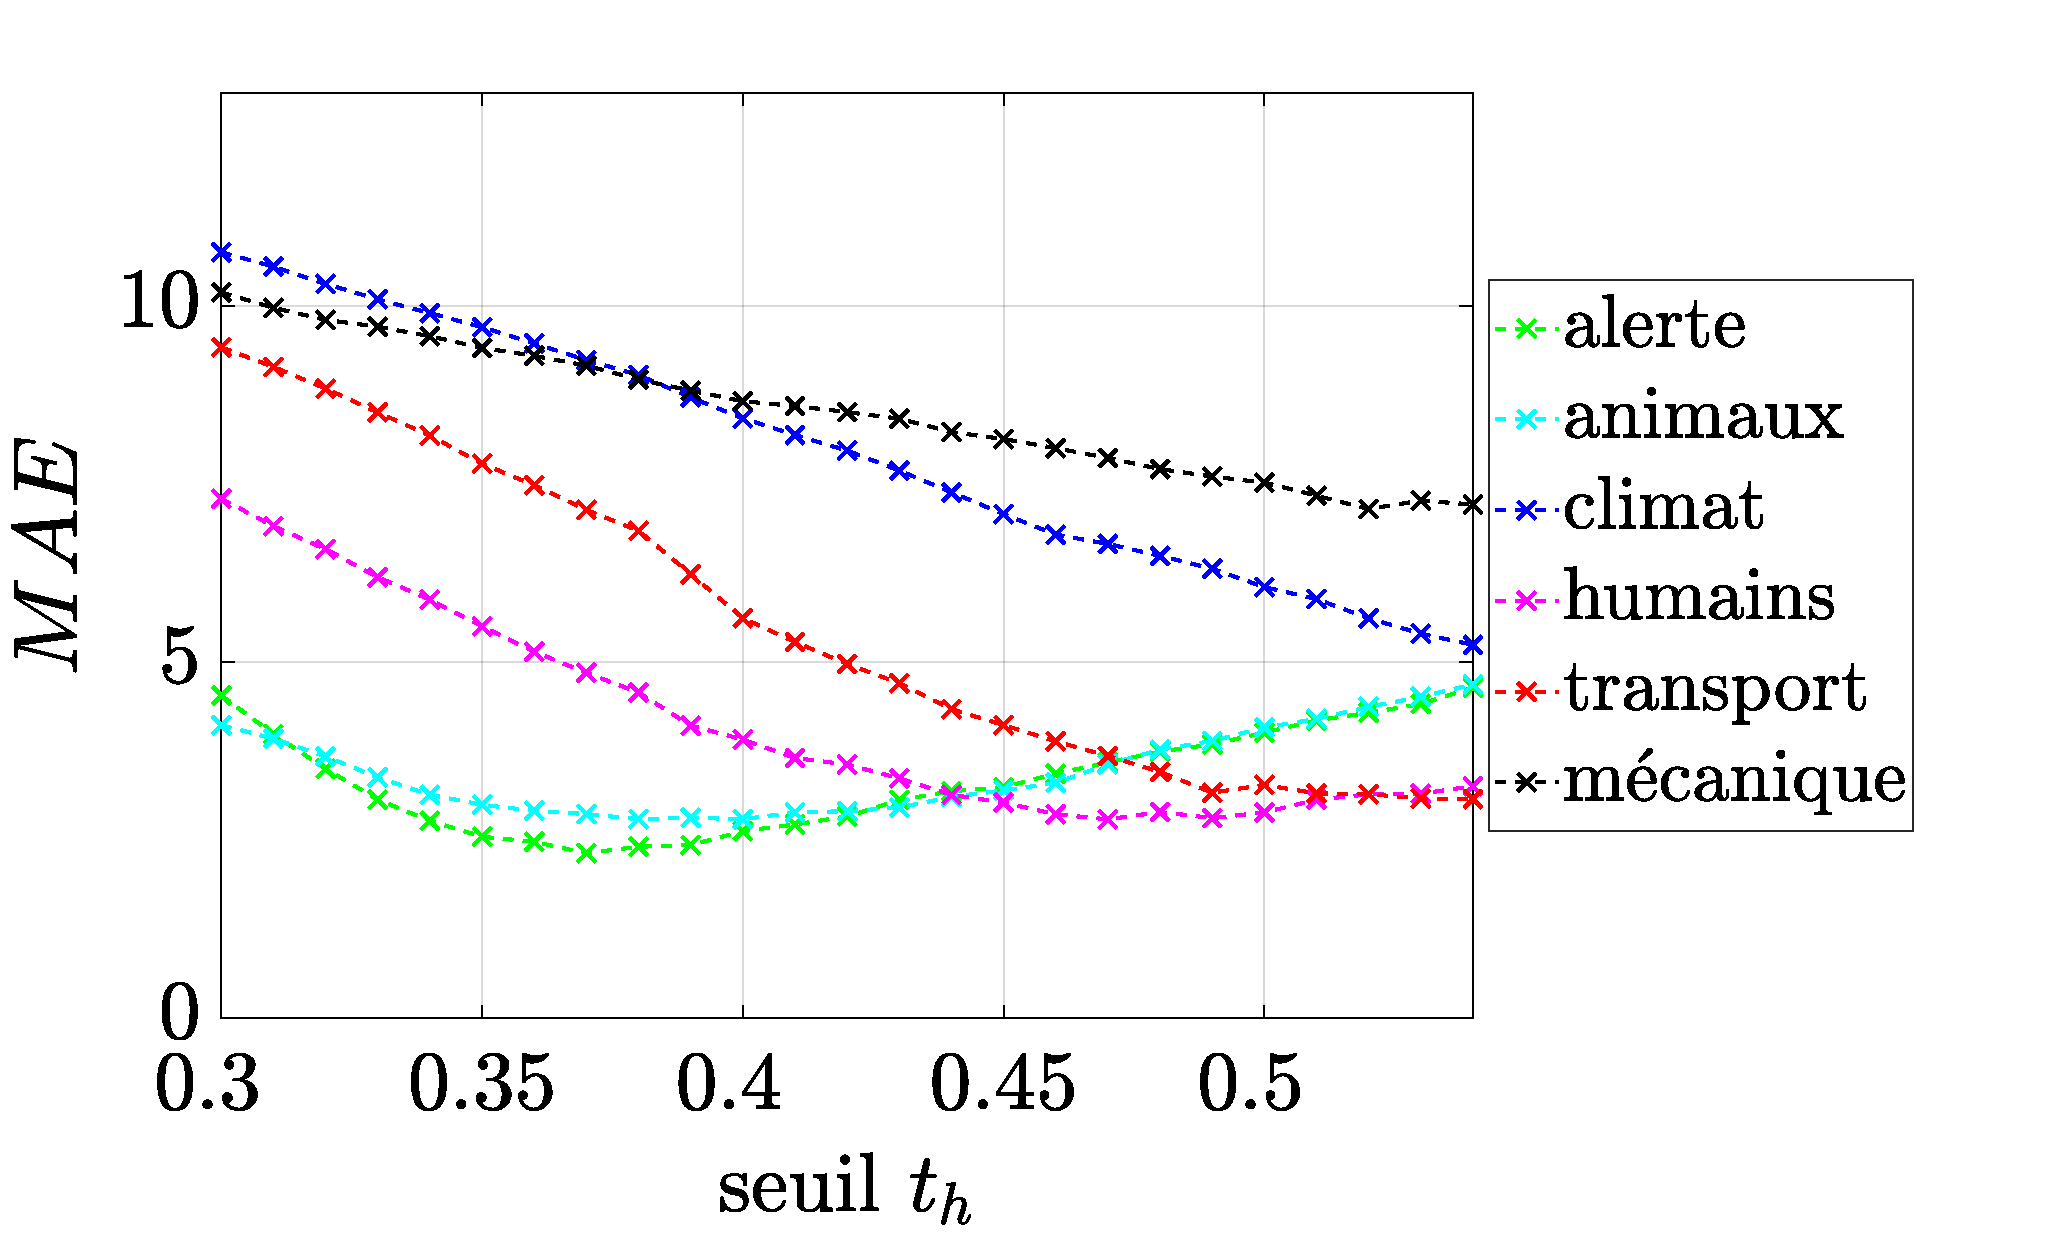
\includegraphics[width=0.60\linewidth]{./figures/resultats/ambiance_maeExpand_tir-12.pdf}}%
\qquad
\subfigure[]{%
\label{fig:TIR_mae_tir0}%
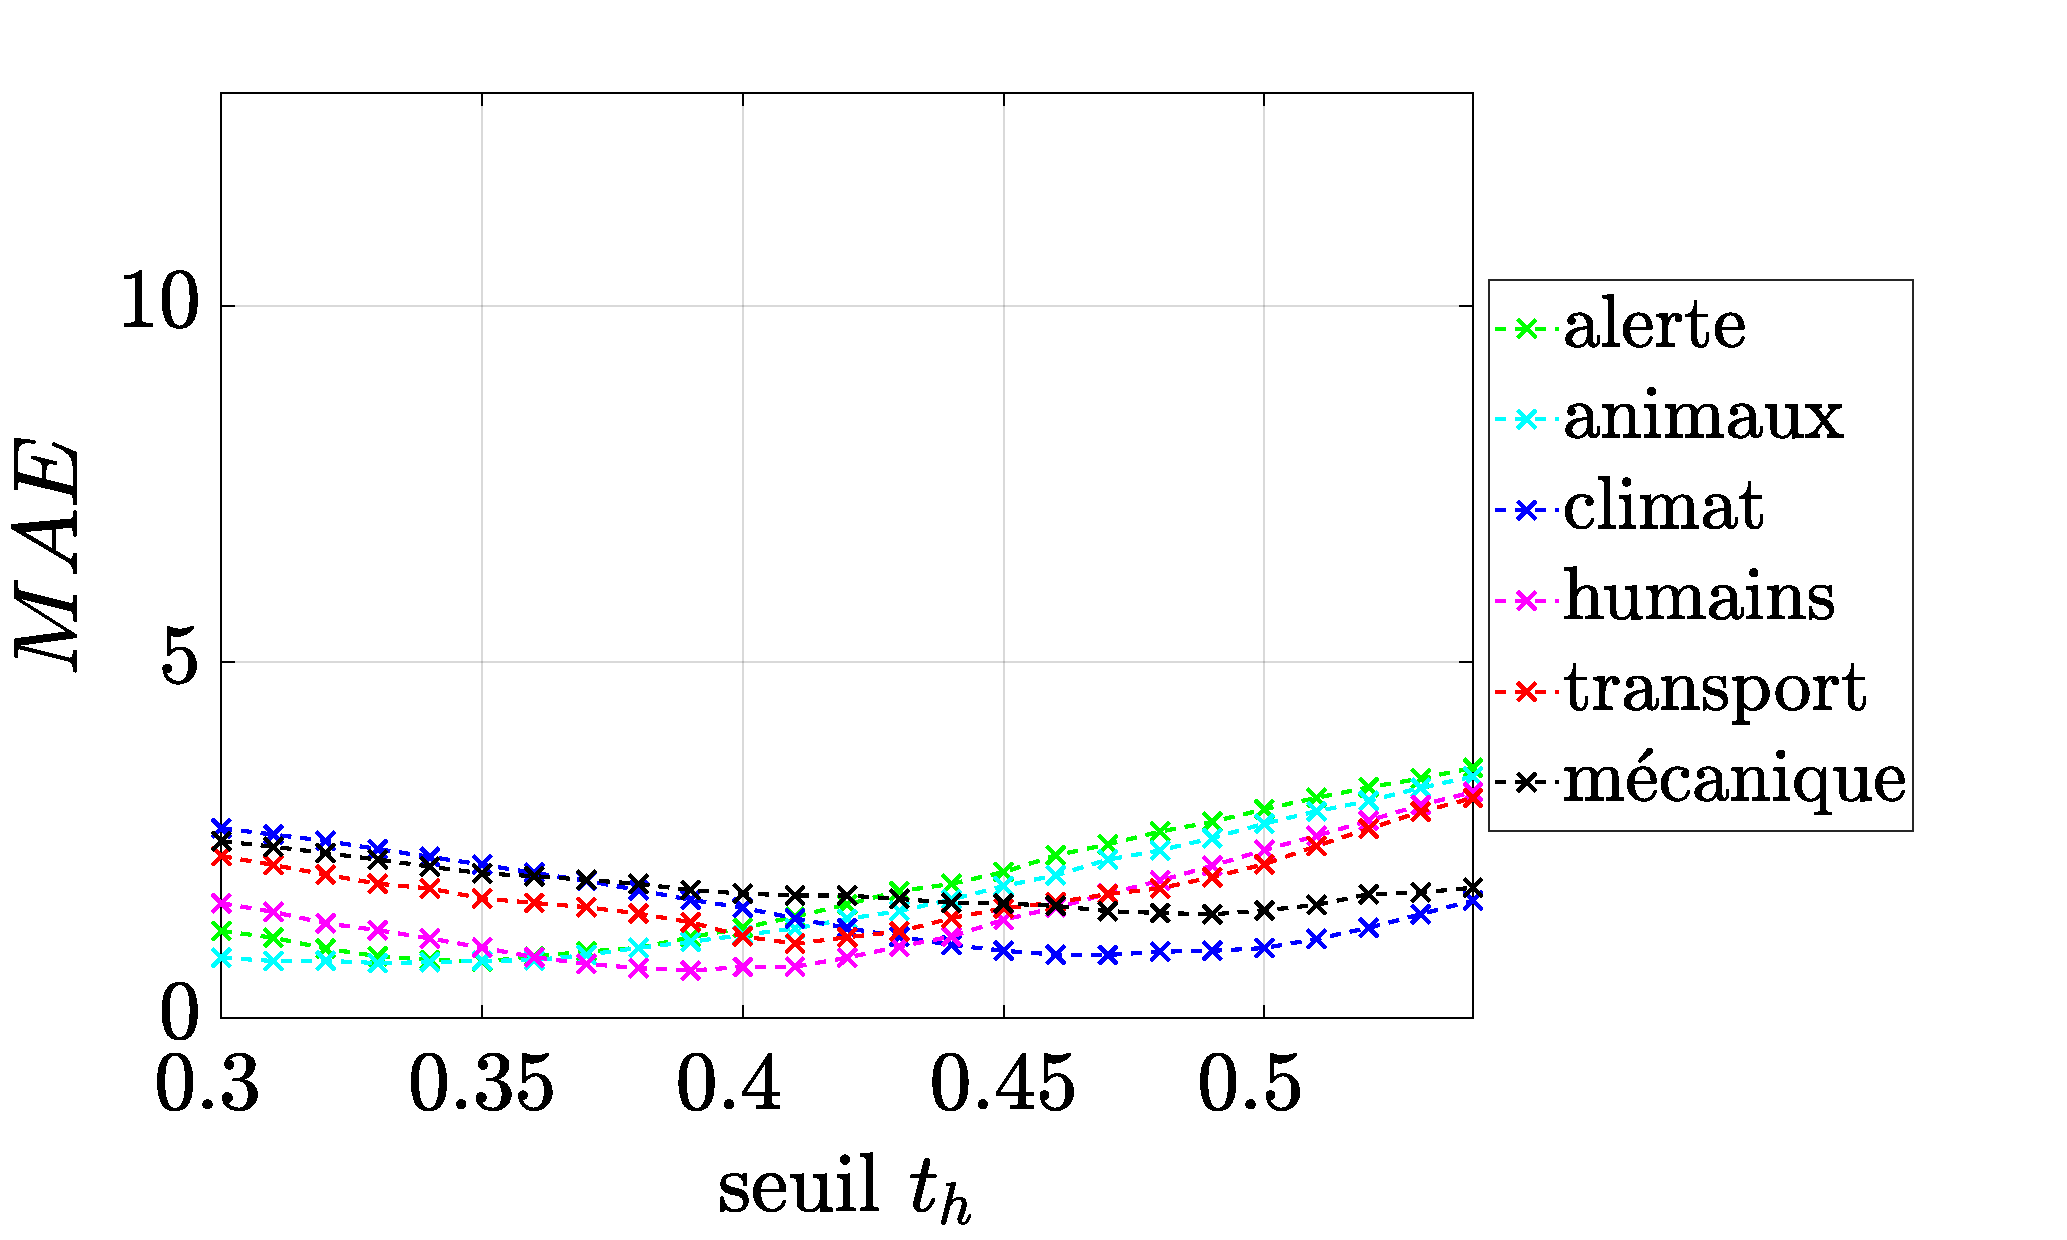
\includegraphics[width=0.60\linewidth]{./figures/resultats/ambiance_maeExpand_tir0.pdf}}%
\qquad
\subfigure[]{%
\label{fig:TIR_mae_tir12}%
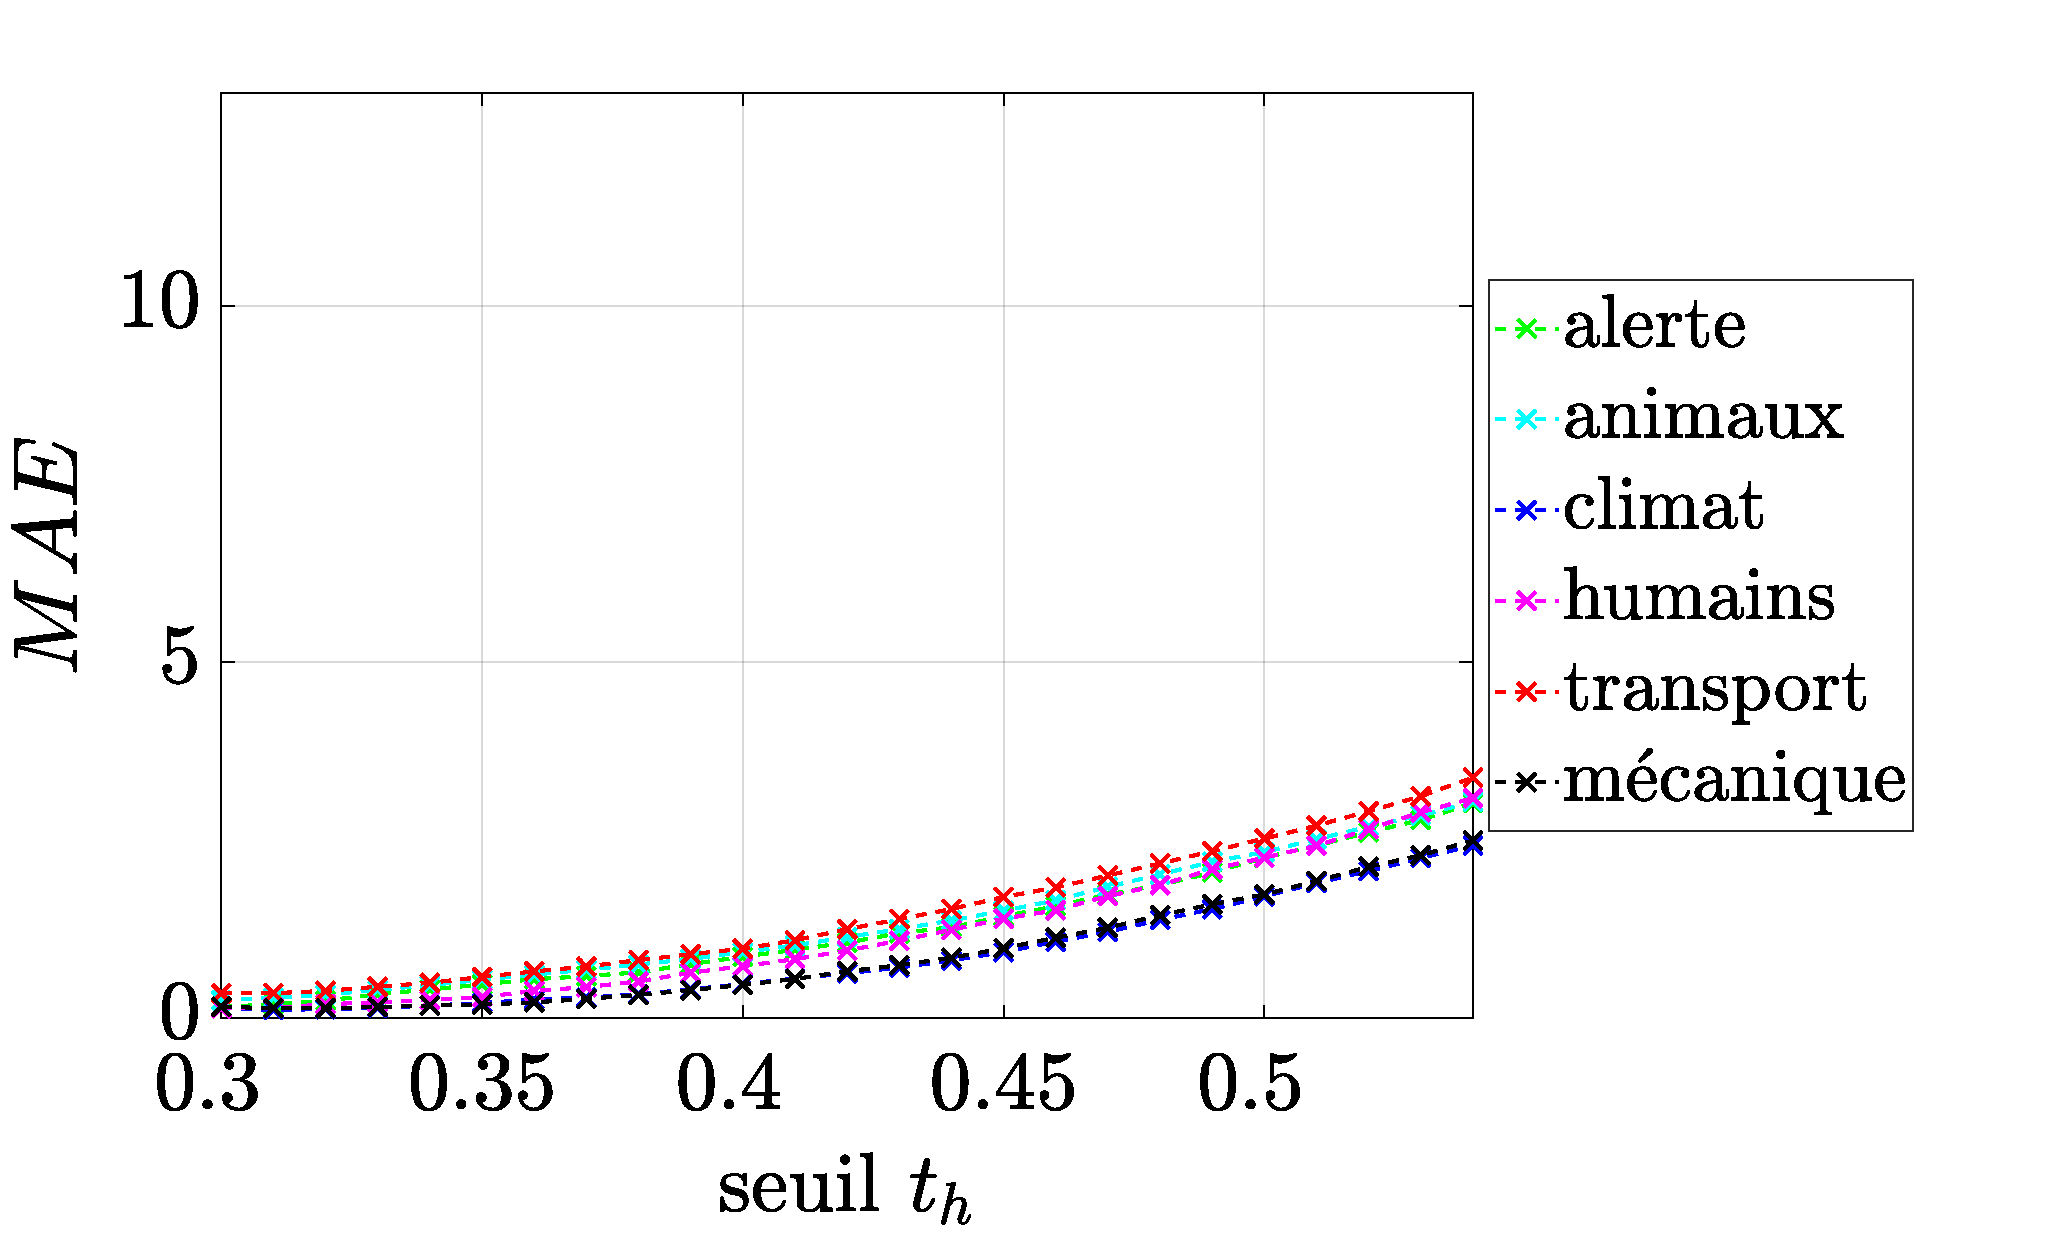
\includegraphics[width=0.60\linewidth]{./figures/resultats/ambiance_maeExpand_tir12.pdf}}%
\caption{Évolution de l'erreur $MAE$ pour chaque sous-corpus selon la valeur seuil $t_h$ pour $TIR = -12$ dB (\ref{fig:TIR_mae_tir-12}), $TIR = 0$ dB (\ref{fig:TIR_mae_tir0}) et $TIR = 12$ dB (\ref{fig:TIR_mae_tir12}).}
\label{fig:TIR_mae}
\end{figure}

\section{Conclusion du chapitre}
Cette première étude, à partir du corpus élémentaire \textit{Ambiance}, a permis d'établir le fonctionnement de plusieurs formes de NMF face à des scènes sonores urbaines. Ces résultats révèlent la difficulté à obtenir une méthode efficace et performante quelque soient les différentes sources sonores interférantes ou la présence variable du trafic.
La NMF SUP, composée d'un dictionnaire comprenant des éléments relatifs au trafic, se révèle être peu performante lorsque le trafic est peu présent en activant des bases \textit{trafic} pour simuler d'autres sources sonores mais est plus efficace lorsque les valeurs du $TIR$ sont positives. La NMF SEM, à l'inverse, est très efficace pour des $TIR$ négatifs, mais échoue à définir correctement le signal \textit{trafic} lorsque cette source sonore devient prédominante. L'ajout du dictionnaire libre $\mathbf{W_r}$ est alors un atout ou un inconvénient selon la prédominance du trafic : dans le premier cas $\mathbf{W_r}$ modélise convenablement la classe de son \textit{interférante} ce qui permet une bonne estimation du niveau sonore du trafic, mais dans le second cas, cet élément du dictionnaire inclut des composantes \textit{trafic} ce qui détériore son estimation. Finalement, la NMF IS se trouve être l'approche qui minimise le mieux l'erreur sur l'ensemble du corpus. Elle réalise un compromis entre les deux méthodes : elle offre suffisamment de liberté par la mise à jour de $\mathbf{W_0}$ pour s'adapter aux différentes ambiances et sources sonores tout en étant contrainte par le seuillage à ne conserver que les éléments les moins divergents. Les différentes pistes étudiées ont permis d'établir que la simple estimation de la distance $D_{\theta}(\mathbf{V}\Vert\mathbf{WH})$ avec l'extraction de la composante \textit{trafic} par seuillage dur est l'approche la plus efficace. \`A la différence des deux autres méthodes, la NMF IS présente l'avantage de modéliser la composante trafic telle qu'elle est capté par le capteur et donc de prendre en compte l'impact de l'environnement. Si on se réfère au problème posé au chapitre \ref{chap:modele} dans la partie \ref{part:problème}, la NMF IS revient à estimer directement le signal $S(t)$ où la composante \textit{trafic}, $S_{tr.}(t)$, est ensuite extraite par la méthode de seuillage dur. La NMF SUP et SEM, quant à elles, tente de déterminer $S_{tr.}(t)$ à partir des connaissances apprises sur la source trafic et donc $s_{tr.}(t)$. La NMF IS présente dont l'intérêt de mieux considérer l'impact de l'environnement sur la source sonore que les deux autres méthodes.\\





%\end{document}
